\documentclass[aps,preprint,preprintnumbers,nofootinbib,showpacs,prd]{revtex4-1}
\usepackage{graphicx,color}
\usepackage{caption}
\usepackage{subcaption}
\usepackage{amsmath,amssymb}
\usepackage{multirow}
\usepackage{amsthm}%        But you can't use \usewithpatch for several packages as in this line. The search 

\usepackage{cancel}

%%% for SLE
\usepackage{dcolumn}   % needed for some tables
\usepackage{bm}        % for math
\usepackage{amssymb}   % for math
\usepackage{multirow}
%%% for SLE -End

\usepackage{ulem}
\usepackage{cancel}

\usepackage{hyperref}

\usepackage[top=1in, bottom=1.25in, left=1.1in, right=1.1in]{geometry}


\newcommand{\msout}[1]{\text{\sout{\ensuremath{#1}}}}


%%%%%% My stuffs - Stef
\newcommand{\lsim}{\mathrel{\mathop{\kern 0pt \rlap
  {\raise.2ex\hbox{$<$}}}
  \lower.9ex\hbox{\kern-.190em $\sim$}}}
\newcommand{\gsim}{\mathrel{\mathop{\kern 0pt \rlap
  {\raise.2ex\hbox{$>$}}}
  \lower.9ex\hbox{\kern-.190em $\sim$}}}

%
% Key
%
\newcommand{\key}[1]{\medskip{\sffamily\bfseries\color{blue}#1}\par\medskip}
%\newcommand{\key}[1]{}
\newcommand{\q}[1] {\medskip{\sffamily\bfseries\color{red}#1}\par\medskip}
\newcommand{\comment}[2]{{\color{red}{{\bf #1:}  #2}}}


\newcommand{\ie}{{\it i.e.} }
\newcommand{\eg}{{\it e.g.} }

%
% Energy scales
%
\newcommand{\ev}{{\,{\rm eV}}}
\newcommand{\kev}{{\,{\rm keV}}}
\newcommand{\mev}{{\,{\rm MeV}}}
\newcommand{\gev}{{\,{\rm GeV}}}
\newcommand{\tev}{{\,{\rm TeV}}}
\newcommand{\fb}{{\,{\rm fb}}}
\newcommand{\ifb}{{\,{\rm fb}^{-1}}}

%
% SUSY notations
%
\newcommand{\neu}{\tilde{\chi}^0}
\newcommand{\neuo}{{\tilde{\chi}^0_1}}
\newcommand{\neut}{{\tilde{\chi}^0_2}}
\newcommand{\cha}{{\tilde{\chi}^\pm}}
\newcommand{\chao}{{\tilde{\chi}^\pm_1}}
\newcommand{\chaop}{{\tilde{\chi}^+_1}}
\newcommand{\chaom}{{\tilde{\chi}^-_1}}
\newcommand{\Wpm}{W^\pm}
\newcommand{\chat}{{\tilde{\chi}^\pm_2}}
\newcommand{\smu}{{\tilde{\mu}}}
\newcommand{\smur}{\tilde{\mu}_R}
\newcommand{\smul}{\tilde{\mu}_L}
\newcommand{\sel}{{\tilde{e}}}
\newcommand{\selr}{\tilde{e}_R}
\newcommand{\sell}{\tilde{e}_L}
\newcommand{\smurl}{\tilde{\mu}_{R,L}}

\newcommand{\casea}{\texttt{IA}}
\newcommand{\caseb}{\texttt{IB}}
\newcommand{\casec}{\texttt{II}}

\newcommand{\caseasix}{\texttt{IA-6}}

%
% Greek
%
\newcommand{\es}{{\epsilon}}
\newcommand{\sg}{{\sigma}}
\newcommand{\dt}{{\delta}}
\newcommand{\kp}{{\kappa}}
\newcommand{\lm}{{\lambda}}
\newcommand{\Lm}{{\Lambda}}
\newcommand{\gm}{{\gamma}}
\newcommand{\mn}{{\mu\nu}}
\newcommand{\Gm}{{\Gamma}}
\newcommand{\tho}{{\theta_1}}
\newcommand{\tht}{{\theta_2}}
\newcommand{\lmo}{{\lambda_1}}
\newcommand{\lmt}{{\lambda_2}}
%
% LaTeX equations
%
\newcommand{\beq}{\begin{equation}}
\newcommand{\eeq}{\end{equation}}
\newcommand{\bea}{\begin{eqnarray}}
\newcommand{\eea}{\end{eqnarray}}
\newcommand{\ba}{\begin{array}}
\newcommand{\ea}{\end{array}}
\newcommand{\bit}{\begin{itemize}}
\newcommand{\eit}{\end{itemize}}

\newcommand{\nbea}{\begin{eqnarray*}}
\newcommand{\neea}{\end{eqnarray*}}
\newcommand{\nbeq}{\begin{equation*}}
\newcommand{\neeq}{\end{equation*}}

\newcommand{\no}{{\nonumber}}
\newcommand{\td}[1]{{\widetilde{#1}}}
\newcommand{\sqt}{{\sqrt{2}}}
%
\newcommand{\me}{{\rlap/\!E}}
\newcommand{\met}{{\rlap/\!E_T}}
\newcommand{\rdmu}{{\partial^\mu}}
\newcommand{\gmm}{{\gamma^\mu}}
\newcommand{\gmb}{{\gamma^\beta}}
\newcommand{\gma}{{\gamma^\alpha}}
\newcommand{\gmn}{{\gamma^\nu}}
\newcommand{\gmf}{{\gamma^5}}
%
% Roman expressions
%
\newcommand{\br}{{\rm Br}}
\newcommand{\sign}{{\rm sign}}
\newcommand{\Lg}{{\mathcal{L}}}
\newcommand{\M}{{\mathcal{M}}}
\newcommand{\tr}{{\rm Tr}}

\newcommand{\msq}{{\overline{|\mathcal{M}|^2}}}

%
% kinematic variables
%
%\newcommand{\mc}{m^{\rm cusp}}
%\newcommand{\mmax}{m^{\rm max}}
%\newcommand{\mmin}{m^{\rm min}}
%\newcommand{\mll}{m_{\ell\ell}}
%\newcommand{\mllc}{m^{\rm cusp}_{\ell\ell}}
%\newcommand{\mllmax}{m^{\rm max}_{\ell\ell}}
%\newcommand{\mllmin}{m^{\rm min}_{\ell\ell}}
%\newcommand{\elmax} {E_\ell^{\rm max}}
%\newcommand{\elmin} {E_\ell^{\rm min}}
\newcommand{\mxx}{m_{\chi\chi}}
\newcommand{\mrec}{m_{\rm rec}}
\newcommand{\mrecmin}{m_{\rm rec}^{\rm min}}
\newcommand{\mrecc}{m_{\rm rec}^{\rm cusp}}
\newcommand{\mrecmax}{m_{\rm rec}^{\rm max}}
%\newcommand{\mpt}{\rlap/p_T}

%%%song
\newcommand{\cosmax}{|\cos\Theta|_{\rm max} }
\newcommand{\maa}{m_{aa}}
\newcommand{\maac}{m^{\rm cusp}_{aa}}
\newcommand{\maamax}{m^{\rm max}_{aa}}
\newcommand{\maamin}{m^{\rm min}_{aa}}
\newcommand{\eamax} {E_a^{\rm max}}
\newcommand{\eamin} {E_a^{\rm min}}
\newcommand{\eaamax} {E_{aa}^{\rm max}}
\newcommand{\eaacusp} {E_{aa}^{\rm cusp}}
\newcommand{\eaamin} {E_{aa}^{\rm min}}
\newcommand{\exxmax} {E_{\neuo \neuo}^{\rm max}}
\newcommand{\exxcusp} {E_{\neuo \neuo}^{\rm cusp}}
\newcommand{\exxmin} {E_{\neuo \neuo}^{\rm min}}
%\newcommand{\mxx}{m_{XX}}
%\newcommand{\mrec}{m_{\rm rec}}
\newcommand{\erec}{E_{\rm rec}}
%\newcommand{\mrecmin}{m_{\rm rec}^{\rm min}}
%\newcommand{\mrecc}{m_{\rm rec}^{\rm cusp}}
%\newcommand{\mrecmax}{m_{\rm rec}^{\rm max}}
%%%song

\newcommand{\mc}{m^{\rm cusp}}
\newcommand{\mmax}{m^{\rm max}}
\newcommand{\mmin}{m^{\rm min}}
\newcommand{\mll}{m_{\mu\mu}}
\newcommand{\mllc}{m^{\rm cusp}_{\mu\mu}}
\newcommand{\mllmax}{m^{\rm max}_{\mu\mu}}
\newcommand{\mllmin}{m^{\rm min}_{\mu\mu}}
\newcommand{\mllcusp}{m^{\rm cusp}_{\mu\mu}}
\newcommand{\elmax} {E_\mu^{\rm max}}
\newcommand{\elmin} {E_\mu^{\rm min}}
\newcommand{\elmaxw} {E_W^{\rm max}}
\newcommand{\elminw} {E_W^{\rm min}}
\newcommand{\R} {{\cal R}}

\newcommand{\ewmax} {E_W^{\rm max}}
\newcommand{\ewmin} {E_W^{\rm min}}
\newcommand{\mwrec}{m_{WW}}
\newcommand{\mwrecmin}{m_{WW}^{\rm min}}
\newcommand{\mwrecc}{m_{WW}^{\rm cusp}}
\newcommand{\mwrecmax}{m_{WW}^{\rm max}}

\newcommand{\mpt}{{\rlap/p}_T}

%%%%%% END My stuffs - Stef

\newcommand{\dunno}{$ {}^{\mbox {--}}\backslash(^{\rm o}{}\underline{\hspace{0.2cm}}{\rm o})/^{\mbox {--}}$}






\begin{document}

\title{Jumbled up thoughts}
\bigskip
\author{Stefanus Koesno$^1$\\
$^1$ Somewhere in California\\ San Jose, CA 95134 USA\\
}
%
\date{\today}
%
\begin{abstract}
Stray thoughts of a stray man. This is a collection of things that I thought was fun to do and also things that I always come back to after forgetting it :) There's no order or structure here just whatever my mind facies at the moment.

\end{abstract}
%
\maketitle

\renewcommand{\theequation}{A.\arabic{equation}}  % redefine the command that creates the equation no.
\setcounter{equation}{0}  % reset counter 
=-=-=-=-=-=-=-=-=-=-=-=-=-=-=-=-=-=-=-=-=-=-=-=-=-=-=-=-=-=-=-=-=-



How does a field and the associated Lagrangian change when we perform a rotation?

Intuitively say we perform an active rotation on the axes themselves and for simplicity we take a small angle rotation around $\hat z$, we'll see that $\hat x$ will get a contribution in $+\hat y$ direction and $\hat y$ will get a contribution in $-\hat x$ direction, see Fig.~\ref{fig:inf-rot}, which means
\nbea
\vec \delta \hat x \Rightarrow +\hat y & = & \hat z \times \hat x \\
\vec \delta \hat y \Rightarrow -\hat x & = & \hat z \times \hat y
\neea
%
\begin{figure}
\begin{center}
  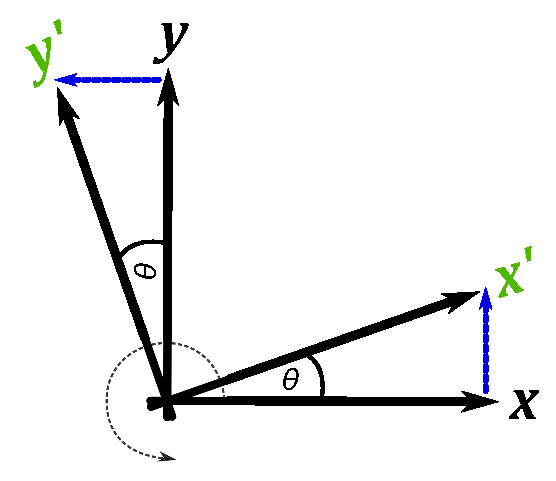
\includegraphics[scale=0.8]{inf-rot.eps}
\end{center}
  \caption{\label{fig:inf-rot}
A rotation of the coordinate axes around the $\hat z$ axis.}
\end{figure}
%
Note that this only works for infinitesimal rotation since for a finite rotation there will be contributions from multiple axes, \eg $\vec \delta x \propto \hat y - \hat x$, if you can't see this just remember the rotation matrix in 2 dimension.

How about a generic rotation axis? say we pick an arbitrary rotation axis $\vec r$ and we want to rotate a vector $\vec A$, remember that the magnitude of $\vec r$ is the amount of rotation, \ie
\nbea
\vec r = a \hat x + b \hat y + c \hat z &\longrightarrow& |\vec r| = \sqrt{a^2 + b^2 + c^2} = \epsilon
\neea

Thus the change in $\vec A$ is given by
\nbea
\vec \delta \vec A = \vec r \times \vec A & = & a (\hat x \times \vec A) + b (\hat y \times \vec A) + c (\hat z \times \vec A)
\neea

Here we see why it only works for infinitesimal rotations since rotations w.r.t different axes do not commute but they only contribute at $\epsilon^2$.

What if instead of a vector we have a scalar $A$? First we need to convert it into a vector, but how? there are many ways of doing it. If we look back to translation $A(x) \rightarrow A(x + \epsilon)$ the transformation we get is $A \rightarrow A + \epsilon \partial A$. Now, we just need to turn this into a vector, the most obvious way is $A \rightarrow A + \vec\epsilon \cdot  (\vec \nabla A)$ (note: we always need a derivative to calculate $\delta A$ thanks to taylor expansion).

Using the formula we have above 
\nbea
\vec \delta (\nabla A) = \vec r \times \nabla A & = & a (\hat x \times \nabla A) + b (\hat y \times \nabla A) + c (\hat z \times \nabla A)
\neea
however the result we have is a vector we need a scalar since $A$ was initially a scalar. The solution is just to take a dot product with $\vec x = \frac{1}{\sqrt{3}}(\hat x + \hat y + \hat z)$
\nbea
\delta A = \vec x \cdot (\vec r \times \nabla A) & = & - \vec r \cdot (\vec x \times \nabla A)
\neea
by using a triple scalar product rule, the thing here now is that I don't know how to get rid of that minus sign LOL

So for a general scalar field you'll get $\delta \phi = \vec \epsilon \cdot (\vec x \times \nabla) \phi$, sans a minus sign, where $\vec x$ is just the coordinate axes and $\vec \epsilon$ is the magnitude and axis of rotation.

Now, how does the lagrangian change? Well, the lagrangian is also a scalar quantity thus we can expect it to also change as $\delta \mathcal{L} =  \vec \epsilon \cdot (\vec x \times \nabla) \mathcal{L}$.

The goal here is to show that $\delta \mathcal{L}$ is related to the stress energy tensor {\it of translation} and for simplicity we will ignore $\vec \epsilon \cdot$ for now
\nbea
(\vec x \times \nabla) \mathcal{L} & = & \epsilon^{ijk} x_j \partial_k \mathcal{L} = \partial_\mu (\epsilon^{ijk} x_j \delta^\mu_k \mathcal{L}) \\
& = & \partial_\mu \mathcal{F}^{\mu i} \\
\rightarrow \mathcal{F}^{\mu i} & = & \epsilon^{ijk} x_j \delta^\mu_k \mathcal{L}
\neea
Since this is a symmetry the change must be a total derivative.

Now from the generic formula for energy stress tensor (under rotation)
\nbea
\widetilde T^{\mu i} & = & \frac{\delta \mathcal{L}}{\delta(\partial_\mu \phi)} \delta \phi - \mathcal{F}^{\mu i} \\
& = & \frac{\delta \mathcal{L}}{\delta(\partial_\mu \phi)} (\vec x \times \vec \nabla) \phi - \epsilon^{ijk} x_j \delta^\mu_k \mathcal{L} \\
& = & \epsilon^{ijk} x_j \left (  \frac{\delta \mathcal{L}}{\delta(\partial_\mu \phi)} \partial_k \phi - \delta^\mu_k \mathcal{L} \right ) =  \epsilon^{ijk} x_j (T^\mu_k) \\
& = & \vec x \times \vec T^\mu
\neea

Notes on energy stress tensor:
Under symmetry transformations, the lagrangian should change by a total derivative (since a symmetry should not change the physics)
\nbea
\delta\mathcal{L} & = & \partial_\mu \mathcal{F}^\mu
\neea 

However the transformation is also given by
\nbea
\delta\mathcal{L} & = & \frac{\delta \mathcal{L}}{\delta\phi}\delta \phi + \frac{\delta \mathcal{L}}{\delta(\partial_\mu \phi)} \delta(\partial_\mu \phi) \\
& = & \partial_\mu \left ( \frac{\delta \mathcal{L}}{\delta(\partial_\mu \phi)} \right ) \delta \phi + \frac{\delta \mathcal{L}}{\delta(\partial_\mu \phi)} \partial_\mu(\delta\phi) \\
\partial_\mu \mathcal{F}^\mu & = & \partial_\mu \left ( \frac{\delta \mathcal{L}}{\delta(\partial_\mu \phi)} \delta \phi \right ) \\
0 & = & \partial_\mu \left ( \frac{\delta \mathcal{L}}{\delta(\partial_\mu \phi)} \delta \phi - \mathcal{F}^\mu \right ) = \partial_\mu J^\mu \\
\rightarrow J^\mu & = & \frac{\delta \mathcal{L}}{\delta(\partial_\mu \phi)} \delta \phi - \mathcal{F}^\mu
\neea
where we have used the equation of motion on the first term going into the second line, this is actually tricky if we apply wrongly we will get something like (doing Integration by parts on the second term at the same time)
\nbea
\delta\mathcal{L} & = & \frac{\delta \mathcal{L}}{\delta\phi}\delta \phi + \frac{\delta \mathcal{L}}{\delta(\partial_\mu \phi)} \delta(\partial_\mu \phi) = \frac{\delta \mathcal{L}}{\delta\phi}\delta \phi - \partial_\mu \left ( \frac{\delta \mathcal{L}}{\delta(\partial_\mu \phi)} \right ) \delta \phi \\
& = & \partial_\mu \left ( \frac{\delta \mathcal{L}}{\delta(\partial_\mu \phi)} \right ) \delta \phi  - \partial_\mu \left ( \frac{\delta \mathcal{L}}{\delta(\partial_\mu \phi)} \right ) \delta \phi \\
& = & 0 ~~~ ???
\neea
LOL indeed but what went wrong? One, we can't really use IBP here since we are not really under an integral. However we can just use the usual trick, $u(dv) = d(uv) - (du)v$
\nbea
\frac{\delta \mathcal{L}}{\delta\phi}\delta \phi + \frac{\delta \mathcal{L}}{\delta(\partial_\mu \phi)} \delta(\partial_\mu \phi) & = & \frac{\delta \mathcal{L}}{\delta\phi}\delta \phi + \partial_\mu \left ( \frac{\delta \mathcal{L}}{\delta(\partial_\mu \phi)} \delta \phi \right ) - \partial_\mu \left ( \frac{\delta \mathcal{L}}{\delta(\partial_\mu \phi)} \right ) \delta \phi \\
& = & \left \{ \frac{\delta \mathcal{L}}{\delta\phi}\delta \phi - \partial_\mu \left ( \frac{\delta \mathcal{L}}{\delta(\partial_\mu \phi)} \right ) \delta \phi \right \} + \partial_\mu \left ( \frac{\delta \mathcal{L}}{\delta(\partial_\mu \phi)} \delta \phi \right ) \\
& = & 0 + \partial_\mu \left ( \frac{\delta \mathcal{L}}{\delta(\partial_\mu \phi)} \delta \phi \right )
\neea
again using the equations of motion for $\phi$.


-=-=-=-=-=-=-=-=-=-=-=-=-=-=-=-=-=-=-=-=-=-=-=-=-=-=-=-=-

In QFT, why does $\phi(x)$ create a particle at spacetime point $x$, \ie $\phi(x)| 0 \rangle = |x \rangle$? For simplicity we'll set $t = 0 \rightarrow \phi(x) = \phi(\vec x, 0)$. To see this take the inner product of
\nbea
\langle \vec x | \vec p \rangle & = & \langle 0 |\phi^\dagger(\vec x, 0) | \vec p \rangle \\
& = & \langle 0 | \left ( \int \frac{d^3 p'}{(2 \pi)^3 \sqrt{\omega_{p'}}} a^\dagger e^{-i\vec {p'} \vec x} +  a e^{i\vec {p'} \vec x} \right ) | \vec p \rangle \\
& = & \left ( \langle 0 | \int \frac{d^3 p'}{(2 \pi)^3 \sqrt{\omega_{p'}}} a e^{i\vec {p'} \vec x} \right ) | \vec p \rangle, ~~~ ( \langle 0 | a^\dagger ) = 0 \\
& = & \int \frac{d^3 p'}{(2 \pi)^3 \sqrt{\omega_{p'}}} e^{i\vec {p'} \vec x} ~~ \{ \langle \vec {p'} | \vec p \rangle \} \\
& = & \int \frac{d^3 p'}{(2 \pi)^3 \sqrt{\omega_{p'}}} e^{i\vec {p'} \vec x} ~~ \left \{ (2 \pi)^3 \sqrt{\omega_{p}} \delta (\vec {p'} - \vec p) \right \} \\
\langle \vec x | \vec p \rangle & = & e^{i\vec {p} \vec x}
\neea
Thus $\phi(x)$ does indeed create a particle at spacetime point $x$ :)

-=-=-=-=-=-=-=-=-=-=-=-=-=-=-=-=-=-=-=-=-=-=-=-=-=-=-=-=-

What is the explicit formula for multiple integrations of a function, \ie what is $\int\int ... \int f(x) dx$ ? The answer is the Cauchy formula for repeated integration
\nbea
(J f)(x) & = & \int_0^x f(t) dt \\
(J^2 f)(x) & = & \int_0^x \left ( \int_0^t f(s) ds \right ) dt \\
(J^\alpha f)(x) & = & \frac{1}{(\alpha - 1)!}\int_0^x (x - t)^{\alpha-1} f(t) dt \\
& = & \frac{1}{\Gamma(\alpha)}\int_0^x (x - t)^{\alpha-1} f(t) dt
\neea
Here we have used $J$ as an integration operator and the identity $\Gamma(\alpha) = (\alpha-1)!$, and also that gamma function can take non integer arguments compared to factorials.

So how do we derive this? The most intuitive derivation I saw was using Laplace transform, some preliminary Laplace transforms that we need are

1. Laplace transform of an integral of a function, $\mathcal{L}\{\int_0^x f(t) dt\}$
\nbea
\mathcal{L}\left \{\int_0^x f(t) dt \right \} & = & \int_0^\infty e^{-sx} \left ( \int_0^x f(t) dt \right ) dx
\neea
we now use integration by parts, $u = \left ( \int_0^x f(t) dt \right ),~dv = e^{-sx} dx $ such that
\nbea
\mathcal{L}\left \{\int_0^x f(t) dt \right \} & = &  \left. \left ( \int_0^x f(t) dt \right ) \frac{e^{-sx}}{(-s)} \right |_{x = 0}^{x = \infty} - \left ( -\frac{1}{s} \right ) \int_0^\infty e^{-sx} f(x) dx \\
& = & 0 + \frac{1}{s} \int_0^\infty e^{-sx} f(x) dx \\
\mathcal{L}\left \{ (J f) (x) \right \} & = & \frac{1}{s}\mathcal{L}\left \{ f(x) \right \} 
\neea
the boundary terms are zero because $\int_0^0 f(t) = 0$ and $e^{-\infty}=0$, assuming $f(t)$ is well behaved. Generalizing to $(J^\alpha f)(x)$ we have
\nbea
\mathcal{L}\left \{ (J^\alpha f) (x) \right \} & = & \frac{1}{s^\alpha}\mathcal{L}\left \{ f(x) \right \} 
\neea

2. Laplace transform of $x^\alpha$, \ie $\mathcal{L}\{x^\alpha\}$ (all function under Laplace transform are assumed to be valid only on the positive real axis)
\nbea
\mathcal{L}\left \{x^\alpha\right \} & = & \int_0^\infty e^{-sx} x^\alpha dx
\neea
here we just need to do multiple integration by parts with $u = x^\alpha,~dv = e^{-sx} dx$
\nbea
\mathcal{L}\left \{x^\alpha\right \} & = &  \left. x^\alpha e^{-sx} \right |_{x=0}^{x=\infty} - \frac{\alpha}{(-s)}\int_0^\infty x^{\alpha-1} e^{-sx} dx \\
& = & \frac{\alpha}{s}\int_0^\infty x^{\alpha-1} e^{-sx} dx
\neea
here we can do 2 things, one use the definition of gamma function $\Gamma(\alpha) = \int_0^\infty x^{\alpha-1} e^{-x} dx$ or repeat the integration by parts again (note that the boundary terms are again zero in this case), if we repeat the IBP $\alpha-1$ more times we get
\nbea
\mathcal{L}\left \{x^\alpha\right \} & = & \frac{\alpha !}{s^\alpha}\int_0^\infty e^{-sx} dx \\
& = & \left. \frac{\alpha !}{s^\alpha} \frac{1}{(-s)} e^{-sx} \right |_{0}^{\infty} \\
& = & -\frac{\alpha !}{s^{\alpha+1}} \left ( e^{-\infty}- e^0\right ) \\
\mathcal{L}\left \{x^\alpha\right \}  & = & \frac{\alpha !}{s^{\alpha+1}}
\neea
which can be generalized to $\mathcal{L}\left \{x^\alpha\right \}  = \frac{\Gamma(\alpha+1)}{s^{\alpha+1}}$ {\it or} just by using the definition of gamma function from the beginning
\nbea
\frac{\alpha}{s}\int_0^\infty x^{\alpha-1} e^{-sx} dx & = & \frac{\alpha}{s}\int_0^\infty \left (\frac{y}{s}\right )^{\alpha-1} e^{-y} \left (\frac{dy}{s} \right), ~~~ y = sx,~ dx = \frac {dy}{s}\\
& = & \frac{\alpha}{s^{\alpha+1}}\int_0^\infty y^{\alpha-1} e^{-y} dy = \frac{\alpha \Gamma(\alpha)}{s^{\alpha+1}},~~~ \alpha \Gamma(\alpha) = \Gamma(\alpha+1)\\
\mathcal{L}\left \{x^\alpha\right \} & = & \frac{\Gamma(\alpha + 1)}{s^{\alpha+1}}
\neea
which is the same result as above.

3. The infamous convolution formula 
\nbea
\mathcal{L}\{f\}\mathcal{L}\{g\} & = & \left (\int_0^\infty e^{-sx} f(x) dx\right )\left (\int_0^\infty e^{-sy} g(y) dy\right ) \\
& = & \int_0^\infty e^{-s(x+y)}  \left ( \int_0^{\infty} f(x) g(y) dy \right ) dx, ~~~ z = x + y \\
& = & \int_0^\infty e^{-s z} \left ( \int_0^{z} f(z-y) g(y) dy \right ) dz \\
\mathcal{L}\{f\}\mathcal{L}\{g\} & = & \mathcal{L} \{ f * g\}
\neea
where $*$ denotes convolution, some explanation on $dx \rightarrow dz$, inside the brackets of $\int dy$, $x$ is constant while outside of this bracket $y$ is {\it constant} and thus $dz = dx$.
 
We are now ready to derive the formula for $(J^\alpha f)(x)$
\nbea
(J^\alpha f)(x) & = & \mathcal{L}^{-1} \{ \mathcal{L} \{J^\alpha f\} \} \\
& = & \mathcal{L}^{-1} \left \{ \frac{1}{s^\alpha} \mathcal{L} \{ f\} \right \} = \mathcal{L}^{-1} \left \{ \frac{\Gamma(\alpha)}{\Gamma(\alpha)}\frac{1}{s^\alpha} \mathcal{L} \{ f\} \right \} \\
& = & \frac{1}{\Gamma(\alpha)}\mathcal{L}^{-1} \left \{ \frac{\Gamma(\alpha)}{s^\alpha} \mathcal{L} \{ f\} \right \} \\
& = & \frac{1}{\Gamma(\alpha)} \left ( \mathcal{L}^{-1} \left \{ \frac{\Gamma(\alpha)}{s^\alpha} \right \} *  f \right ) \\
& = & \frac{1}{\Gamma(\alpha)} \left ( x^{\alpha-1} *  f \right ) \\
(J^\alpha f)(x) & = & \frac{1}{\Gamma(\alpha)} \int_0^x ( x - t )^{\alpha-1}  f(t) dt 
\neea
which is the Cauchy formula we were looking for.

-=-=-=-=-=-=-=-=-=-=-=-=-=-=-=-=-=-=-=-=-=-=-=-=-=-=-=-=-

{\bf Problem 1.1 Srednicki, Show that the Dirac matrices must be even dimensional. Hint: show that the eigenvalues of $\beta$ are all $\pm 1$, and that ${\rm Tr} \beta = 0$. To show that ${\rm Tr} \beta = 0$, consider \eg ${\rm Tr} \alpha_1^2 \beta$. Similarly, show that ${\rm Tr} \alpha_i = 0$.}

Some facts about Dirac matrices
%
\nbea
\{ \alpha^j, \alpha^k\}_{ab} = 2\delta^{jk}\delta_{ab} ~~~ \{ \alpha^j, \beta\}_{ab} = 0 ~~~ (\beta)^2_{ab} = \delta_{ab}
\neea
%
For eigenvalues of $\beta$ it follows immediately from $(\beta)^2_{ab} = \delta_{ab}$ its eigenvalues must be $\pm 1$.

For ${\rm Tr} \beta$ we start with
%
\nbea
{\rm Tr} (\alpha_1^2 \beta) & = & {\rm Tr} (\alpha_1 \beta \alpha_1), ~~\{ \alpha^j, \beta\}_{ab} = 0 \\
& = & {\rm Tr} (-\beta \alpha_1 \alpha_1) \\
{\rm Tr} (\alpha_1^2 \beta) & = & {\rm Tr} (\beta  \alpha_1 \alpha_1), ~~{\rm Tr}(AB) = {\rm Tr}(BA) \\
\rightarrow {\rm Tr} (-\beta \alpha_1 \alpha_1) & = & {\rm Tr} (\beta \alpha_1 \alpha_1) \\
{\rm Tr} (\beta \alpha_1 \alpha_1) & = & 0
\neea
%
Now from $\{ \alpha^j, \alpha^k\}_{ab} = 2\delta^{jk}\delta_{ab} \rightarrow \{ \alpha_i, \alpha_i\}_{ab} = 2 \delta_{ab}$, it means that $(\alpha^2_i)_{ab} = \delta_{ab}$ and thus ${\rm Tr} (\beta \alpha_i \alpha_i) = {\rm Tr} (\beta) = 0$.

Now since ${\rm Tr} \beta = 0$ and its eigenvalues are $\pm 1$, $\beta$ must be even dimensional.

This argument applies for ${\rm Tr} \alpha_i$ as well by reversing the roles of $\beta$ and $\alpha$, ${\rm Tr} (\beta^2 \alpha_i) = {\rm Tr} (\alpha_i) = 0$ and since $(\alpha^2_i)_{ab} = \delta_{ab} \rightarrow$ eigenvalues must be $\pm 1$, $\alpha^i$ must be even dimensional. This means that {\it all} of Dirac matrices must be even dimensional.

Now we need to show that Dirac matrices must be bigger than $2 \times 2$. I'll start with the fact that any $2 \times 2$ matrix can be written as $ a_0 1 + a_i \sigma^i$, \ie a combination of Pauli matrices and the identity matrix. If you remember some sort of group theory, the group $su(2)$ spans a three sphere and the basis vectors (lie algebra $SU(2)$) are spanned by the Pauli matrices.

The commutation relations of Pauli matrices are
%
\nbea
\{\sigma^i, \sigma^j\}_{ab} & = & 2\delta^{ij} \delta_{ab} \\
\lbrack \sigma^i, \sigma^j \rbrack & = & 2 i \varepsilon^{ijk} \sigma^{k} 
\neea
%
As we can see from their anticommutation relations, the pauli matrices can play the role of $\alpha^i$. We now need to show that there are no fourth $2\times2$ matrix to play the role of $\beta$. To do this let's construct a generic $2\times2$ matrix $A = a_0 1 + a_i \sigma^i$ and do its commutation relation with the pauli matrices and see what coefficients $(a_0, a_i)$ we need to fulfill the commutation relation $\{ \alpha^j, \beta\}_{ab} = 0$
%
\nbea
\{A, \sigma^j\} & = & \{a_0 1 + a_i \sigma^i,  \sigma^j\} \\
0 & = & \{a_0 1,  \sigma^j\}  + \{a_i \sigma^i,  \sigma^j\} \\
0 & = & 2 a_0 \sigma^j + a_i \delta^{ij} 1 \\
0 & = & 2 a_0 \sigma^j + a_j 1
\neea
%
Recall that there's only one diagonal pauli matrix, \ie if you use $\hat z$ as the main direction $\sigma_z = (+1, -1)$ which is just spin up and spin down and the other two pauli matrices will be off diagonal, if you choose any other axis the same will occur, only one will be diagonal and the other two will be off diagonal.

From $0 = 2 a_0 \sigma^j + a_j 1$, we need $\sigma^j$ to be diagonal but since $\sigma^j = (+1, -1)$ the only solution is $a_0 = 0, a_j = 0$. However the anticommutation relation $\{A, \sigma^j\} = 0$ has to be true for all values of $j = 1,2,3$ which means that $a_1 = a_2 = a_3 = 0 \rightarrow A = 0$, so the only $2\times2$ matrix that can fulfill the role of $\beta$ is the zero matrix. However, $\beta^2 = 1$, hence Dirac matrices must be at least $4\times4$.

-=-=-=-=-=-=-=-=-=-=-=-=-=-=-=-=-=-=-=-=-=-=-=-=-=-=-=-=-

{\bf Srednicki Problem 4.1 Verify eq. (4.12). Verify its limit as $m \rightarrow 0$. Eq. 4.12 is $\lbrack \varphi^+(x),\varphi^-(x') \rbrack = (m/4\pi^2 r) K_1(mr) \equiv C(r)$ where $K_1(mr)$ is a modified Bessel function of the second kind.}

The subject here is that for a transition amplitude to be Lorentz invariance, the above commutator must be zero, however it's not. Why does it have to be zero? because the transition amplitude is given by time ordered product of the fields and for spacelike separations, $x-x' > 0$, the time ordering might shuffle the order of the fields as for a spacelike separation different observers might see two events happen in different orders. Note that the metric used here is $(-+++)$. Hence the need to set $\lbrack \varphi^+(x),\varphi^-(x') \rbrack = 0$ to maintain equal transition amplitudes for all observers, $\langle \varphi(x) \varphi(y) \rangle = \langle \varphi(y) \varphi(x) \rangle$.

However, eq. 4.12 shows that $\lbrack \varphi^+(x),\varphi^-(x') \rbrack \neq 0$! Our task at hand is to derive this conclusion. First we need to choose a frame where $t-t'=0$ as suggested by the text to simplify calculation.
%
\nbea
\int \widetilde{dk} ~e^{ik(x-x')} & = & \int \frac{d^3k}{(2 \pi)^3 2 \sqrt{k^2 + m^2}} e^{(-ik_0 \Delta t + i \vec k \cdot \Delta \vec x)}, ~\Delta t = 0 \\
& = &  \int \frac{d^3k}{(2 \pi)^3 2 \sqrt{k^2 + m^2}} e^{(i\vec k \cdot \Delta \vec x)}\\
& = &  \int \frac{d^3k}{(2 \pi)^3 2 \sqrt{k^2 + m^2}} e^{i|k||r| \cos \theta}, ~ |r| = |\Delta \vec x|\\
& = &  \int \frac{k^2 dk~ d\phi~ d(\cos\theta)} {(2 \pi)^3 2 \sqrt{k^2 + m^2}} e^{i|k||r| \cos \theta}\\
& = &  \int \frac{k^2 dk~ \bcancel{2 \pi}} {(2 \pi)^{\bcancel{3}2} 2 \sqrt{k^2 + m^2}} \int^1_{-1} d(\cos\theta)~e^{i|k||r| \cos \theta}\\
& = &  \int \frac{k^2 dk} {(2 \pi)^2 2 \sqrt{k^2 + m^2}} \frac{(e^{i|k||r|} - e^{-i|k||r|})}{ikr}\\
& = &  \int \frac{k dk} {(2 \pi)^2 \bcancel{2} \sqrt{k^2 + m^2}} \frac{\bcancel{2}\bcancel{i}\sin(k r)}{\bcancel{i}r}\\
& = &  \frac{1} {(2 \pi)^2 r} \int_0^\infty dk \frac{k \sin(k r)} {\sqrt{k^2 + m^2}} 
\neea
%
We now need to massage this into a Bessel function, but first let's do a change of variable $ \rightarrow y = k/m$
%
\nbea
& = &  \frac{1} {(2 \pi)^2 r}  \int_0^\infty m ~d\left(\frac{k}{m}\right) \frac{m \left(\frac{k}{m}\right) \sin(\left(\frac{k}{m}\right) m r)} {m \sqrt{\left(\frac{k}{m}\right)^2 + 1}} \\
& = &  \frac{m} {(2 \pi)^2 r}  \int_0^\infty dy \frac{y \sin(y m r)} {\sqrt{y^2 + 1}} 
\neea
%
now, there are 2 facts we need about Bessel functions
%
\nbea
K_0(z) & = & \int_0^\infty dy \frac{\cos(zy)}{\sqrt{y^2 + 1}} \\
\frac{d}{dz} K_\nu(z) & = & \frac{\nu}{z} K_{\nu}(z) - K_{\nu+1}(z) \\
\rightarrow \frac{d}{dz} K_0(z) & = & - K_{1}(z)
\neea
%
If we do the actual derivative on $K_0$ we get
%
\nbea
\rightarrow \frac{d}{dz} K_0(z) & = & \int_0^\infty dy \frac{d}{dz} \left (\frac{\cos(zy)}{\sqrt{y^2 + 1}} \right ) \\
- K_{1}(z) & = & - \int_0^\infty dy \frac{y \sin(zy)}{\sqrt{y^2 + 1}} \\
\rightarrow \frac{m} {(2 \pi)^2 r} K_{1}(z) & = & \frac{m} {(2 \pi)^2 r} \int_0^\infty dy \frac{y \sin(zy)}{\sqrt{y^2 + 1}}, ~ z \rightarrow mr \\
\frac{m} {4 \pi^2 r} K_{1}(mr) & = & \frac{m} {(2 \pi)^2 r} \int_0^\infty dy \frac{y \sin(mr y)}{\sqrt{y^2 + 1}} \\
\frac{m} {4 \pi^2 r} K_{1}(mr) & = & \int \widetilde{dk} ~e^{ik(x-x')}
\neea
%
and that is the result that we want. How about its limit as $m \rightarrow 0$? One might be tempted to find or calculate the power series expansion of the Bessel function around $z \rightarrow 0$ but I found it extremely difficult (as I've forgotten most of the methods from my mathematical methods class) but (after looking at the problem long enough) I realized that we need not mess with Bessel functions at all.

You see $\int \widetilde{dk} ~e^{ik(x-x')}$ looks a lot like a fourier transform and setting $m \rightarrow 0$ makes it look like this
%
\nbea
& = &  \int \frac{d^3k} {(2 \pi)^3 2 \sqrt{k^2 + m^2}} e^{i \vec k \cdot \vec r}, ~m \rightarrow 0\\
& = &  \frac{1}{2 (2 \pi)^3} \int d^3k \frac{e^{i \vec k \cdot \vec r}}{|k|}
\neea
%
which looks a lot like the fourier transform of the Coulomb potential but this time it's going into the $\vec x$ domain instead of the $\vec k$ domain.

The evaluation of this integral is usually done using a regulator $e^{-\mu k}$ and we'll take the limit $\mu \rightarrow 0$ at the end.
%
\nbea
& = & \frac{1}{2 (2 \pi)^3} \int d^3k \frac{e^{-\mu k} e^{i \vec k \cdot \vec r}}{|k|} \\
& = & \frac{1}{2 (2 \pi)^3} \int k^{\bcancel{2}} dk ~ d\phi~ \frac{e^{-\mu k}}{\bcancel{k}} \int_{-1}^1 d(\cos\theta) e^{i |k| |r| \cos \theta} \\
& = & \frac{1}{2 (2 \pi)^2} \int_0^\infty \bcancel{k} dk ~ e^{-\mu k} \frac{(e^{i k r} - e^{-i k r})}{i \bcancel{k} r} \\
& = & \frac{1}{2 i r (2 \pi)^2} \int_0^\infty dk ~ e^{-\mu k} (e^{i k r} - e^{-i k r}) \\
& = & \frac{1}{2 i r (2 \pi)^2} \left \lbrack \frac{1}{(-\mu + ir)} \left. e^{(-\mu + i r)k} \right |_0^\infty - \frac{1}{(-\mu - ir)} \left. e^{(-\mu - i r)k} \right |_0^\infty \right \rbrack \\
& = & \frac{1}{2 i r (2 \pi)^2} \left \lbrack \frac{1}{(-\mu + ir)} (e^{-\infty} - e^0 ) - \frac{1}{(-\mu - ir)} (e^{-\infty} - e^0 ) \right \rbrack \\
& = & \frac{1}{2 i r (2 \pi)^2} \left \lbrack \frac{1}{(-\mu - ir)} - \frac{1}{(-\mu + ir)} \right \rbrack =  \frac{1}{2 i r (2 \pi)^2} \left \lbrack \frac{-\mu + ir + \mu + ir}{\{(-\mu)^2 - (ir)^2\}} \right \rbrack \\
& = & \frac{1}{\bcancel{2 i r} (2 \pi)^2} \frac{\bcancel{2 i r}}{\{(-\mu)^2 + r^2\}}, ~\mu \rightarrow 0 \\
& = & \frac{1}{4 \pi^2 r^2}
\neea
%
which is the result we want :) without messing with Bessel functions at all

-=-=-=-=-=-=-=-=-=-=-=-=-=-=-=-=-=-=-=-=-=-=-=-=-=-=-=-=-

How do you do the integral of $\int_{-\infty}^{\infty} dx \frac{\sin x}{x}$? The common solution is to do a contour integration, but is there another way? This was what I attempted, the answer to that question is in short no, but I sure learned a hell lot thinking about this problem.

First, there's no function whose derivative is $\frac{\sin x}{x}$ which means that the indefinite integral $\int dx \frac{\sin x}{x}$ has no solution. Contour integral was a neat technique apropos to a numerical calculation.

My original approach was inspired by green's function method. This was because the integral $\int dx \frac{\sin x}{x}$ is akeen to $\int dk \frac {e^{ikx}}{k}$ and since $\cos k$ is even, only the $\sin k$ term will survive the integration $\rightarrow \int dk \frac {i\sin (kx)}{k}$ and by taking $x \rightarrow 1$ we'll get $\int dk \frac{i \sin k}{k}$ which is what we want. The starting point is the unit step function $u(x)$
%
\nbea
\frac{d}{dx} u(x) & = & \delta(x) \\
\rightarrow ik ~ u(k) & = & 1 \\
u(k) & = & \frac{1}{ik}
\neea
%
We must take a pause here. First some trivial things, I have chosen the fourier transform pair to be $f(x) = \frac{1}{2\pi} \int dk e^{ikx} F(k)$ and $F(k) = \int dx e^{-ikx} f(x)$, \ie we put all factor of normalization $\frac{1}{2\pi}$ in the inverse transform. We can choose other normalization schemes, but the result will be the same.

The second reason to pause here is more serious. The unit step function is a peculiar function. Note that
%
\nbea
\frac{d}{dx}  \left ( u(x) + C \right ) & = & \delta(x)
\neea
%
is still true for any constant $C$. But there's a particular value of $C$ that has serious ramifications, \ie $C = -\frac{1}{2}$. Why? because
%
\nbea
\left (u(x) - \frac{1}{2} \right ) & = & \frac{1}{2} \left ( u(x) - u(-x) \right )
\neea
%
that is $\left (u(x) - \frac{1}{2} \right )$ is just the antisymmetric part of $u(x)$. Now there is a fact that we need to remember, an antisymmetric (real) function has as its fourier counterpart a purely imaginary function $\int dx e^{-ikx} f(x) = -i\int dx \sin(kx) f(x)$. We see above that $u(k) = \frac{1}{ik}$ (purely imaginary) and since $\frac{d}{dx} u(x) = \frac{d}{dx}  \left ( u(x) + C \right )$ what we were really doing was fourier transforming only the antisymmetric part of $u(x)$, \ie
%
\nbea
\frac{d}{dx}  \left ( \frac{1}{2} (u(x) - u(-x)) \right ) & = & \frac{d}{dx}  \left ( u(x) - \frac{1}{2} \right )  = \delta(x) \\
\mathcal{F}\left \{ \frac{d}{dx}  \left ( u(x) - \frac{1}{2} \right ) \right \} & = & \mathcal{F}\left \{ \delta(x) \right \} \\
ik ~\mathcal{F} \left \{ \left ( u(x) - \frac{1}{2} \right ) \right \} & = & 1 \\
ik \left ( u(k) - \frac{1}{2} (2\pi \delta(k)) \right ) & = & 1 \\
u(k) & = & \frac{1}{ik} + \pi \delta(k)
\neea
%
Note that $\mathcal{F}\left \{ \delta(x) \right \} = 1$ and $\mathcal{F}\left \{ 1 \right \} = 2\pi \delta(k)$ is affected by the normalization scheme, other schemes will produce different numerical factors. Now, what does it have to do with $\int dx \frac{\sin x}{x}$? Let's do an inverse fourier transform on the above function
%
\nbea
\mathcal{F}^{-1}\left \{ u(k) \right \} & = & \mathcal{F}^{-1}\left \{ \frac{1}{ik} + \pi \delta(k) \right \} \\
u(x) & = & \frac{1}{2\pi} \int_{-\infty}^{\infty} dk \frac{e^{ikx}}{ik} + \frac{1}{2\bcancel{\pi}} \int_{-\infty}^{\infty} dk~e^{ikx} \left ( \bcancel{\pi} \delta(k) \right ) \\
u(x) & = & \frac{1}{2\pi i} \int_{-\infty}^{\infty} dk \frac{e^{ikx}}{k} + \frac{1}{2}
\neea
%
Now we set $x \rightarrow 1, u(1) = 1$
%
\nbea
u(1) & = & \frac{1}{2\pi i} \int_{-\infty}^{\infty} dk \frac{e^{ik}}{k} + \frac{1}{2} \\
1 & = & \frac{1}{2\pi \bcancel{i}} \int_{-\infty}^{\infty} dk \frac{\bcancel{i} \sin k}{k} + \frac{1}{2} \\
\rightarrow \int_{-\infty}^{\infty} dk \frac{\sin k}{k} & = & \pi
\neea
%
In the second line we have used the fact that since $\frac{\cos k}{k}$ is an odd function, its integral is zero. And this is the origin of the factor of $\pi$. For the longest time I have wondered how this integral has anything to do with $\pi$. But wait, you might ask how in turn did the fourier transform pair acquire this factor of $\frac{1}{2\pi}$ in the first place?

The answer to that question is the gaussian integral $e^{-x^2/2}$. This gaussian function is the eigenfunction of the fourier transform. Let's see how it works
%
\nbea
\int_{-\infty}^{\infty} dx~ e^{-ikx} e^{-x^2/2} & = & \sqrt{2 \pi} ~e^{\frac{(-ik)^2}{4\left( \frac{1}{2} \right)}} \\
& = & \sqrt{2 \pi} ~e^{-k^2/2}
\neea
%
where we have used the gaussian integral formula $\int dx~e^{-ax^2 + bx + c} = \sqrt{\frac{\pi}{a}} e^{\frac{b^2}{4a} + c}$ and if we do an inverse transform we get
%
\nbea
\int_{-\infty}^{\infty} dk~ e^{ikx} \left ( \sqrt{2 \pi} ~e^{-k^2/2} \right ) & = & \sqrt{2 \pi}\sqrt{2 \pi}~ e^{\frac{(ix)^2}{4\left( \frac{1}{2} \right)}} \\
& = & 2 \pi ~e^{-x^2/2}
\neea
%
Thus
%
\nbea
\mathcal{F}^{-1} \left \{ \mathcal{F} \left \{ e^{-x^2/2}\right \} \right \} & = & 2 \pi ~e^{-x^2/2}
\neea
%
or equivalently
%
\nbea
e^{-(0)^2/2} & \stackrel{\text{\tiny ?}}{=} & \int_{-\infty}^{\infty} dk~ e^{ik(0)} \left ( \sqrt{2 \pi} ~e^{-k^2/2} \right ) \\
& = & \sqrt{2 \pi} \int_{-\infty}^{\infty} dk~e^{-k^2/2} =  \sqrt{2 \pi} \sqrt{2 \pi} \\
1 & \stackrel{\text{\tiny ?}}{=} & 2 \pi
\neea
%
this means that we need to absorb the extra factor of $2 \pi$ somehow, the usual way is to put a $\frac{1}{2\pi}$ in the inverse transform, another common way is to put a factor of $\frac{1}{\sqrt{2 \pi}}$ on both the fourier transform and its inverse. Note that my derivation of $\int \frac{\sin k}{k}$ does not depend on the normalization scheme, you might try it if you don't believe me ;)

But then again, how did the gaussian integral get a factor of $\pi$, well it's because we use a circle to compute it, remember?
%
\nbea
\int_{-\infty}^{\infty} e^{-x^2/2} & = & \sqrt {\left ( \int_{-\infty}^{\infty} e^{-x^2/2} \int_{-\infty}^{\infty} e^{-y^2/2}\right ) } \\
& = & \sqrt { \int_{-\infty}^{\infty} dx dy ~ e^{-(x^2 + y^2)/2}} \\
& = & \sqrt { \left ( \int_0^{2\pi} d\phi \right )\int_{0}^{\infty} r dr  ~ e^{-(r^2)/2}} \\
\int_{-\infty}^{\infty} e^{-x^2/2} & = & \sqrt {2 \pi}
\neea
%
And that my friend, is how you get a factor of $\pi$ in the first place :) Of course in the contour integration of $\int \frac{\sin x}{x}$ the factor of $\pi$ is due to the infinitesimal semi circle around $x=0$ but again, it's all due to a circle.

It took me two days to figure this out and I learned a lot about the step function and fourier transform in the process. It all started with a simple thought of whether or not it's possible to compute $\int \frac{\sin x}{x}$ wihout contour integration, turns out that it's not quite possible, sometimes we do need a new technique to solve an old problem and I gained a new respect for complex numbers.

%how to strike out texts
%$\msout{\mathsf{stuckout}}$

%$\cancel{5}$

%$\bcancel{5}$
-=-=-=-=-=-=-=-=-=-=-=-=-=-=-=-=-=-=-=-=-=-=-=-=-=-=-=-=-

Why do we need limits and what are they? Let's start with the infamous $\stackrel{\mbox{lim}}{_{x \to 0}}$. Without messing with $\delta$ and $\epsilon$ as in the usual formal definition of a limit, what a limit amounts to is (in the case $x \to 0^{+}$, \ie we're approaching the limit from the right) $\stackrel{\mbox{lim}}{_{~~x \to 0^+}}$ $\Rightarrow x > 0$ but $x$ is smaller than any positive real number.

Now how can that be? If it is smaller than any positive real number (and it's not negative) then it has to be zero. One way it is possible if we are dealing with infinities, something like 
% a sample tex on how to do horizontal curly braces
%z = \overbrace{
%    \underbrace{x}_\text{real} +
%    \underbrace{iy}_\text{imaginary}
%   }^\text{complex number}
%
\nbea
x = 0.\underbrace{000000 ~...~ 00000}_\text{infinite \# of zeros}1
\neea
%
There are an infinite number of zeros before the digit $1$ so that it doesn't matter how small the real number you present me, I can always produce a smaller one by adding more zeros in between and it has to be infinite for this to work because $x$ is smaller than {\it any} positive real number. But this won't work since it is just zero! Remember that
%
\nbea
1 = 0.\underbrace{999999 ~...~ 99999}_\text{infinite \# of 9's}
\neea
%
Thus limits are a (more severe?) manifestation of infinities. The real question is: why do we need it? The more obvious reason is in the calculation of a slope. To calculate a slope you need at least two points, say $(x_1, y_1)$ and $(x_2, y_2)$ and the slope is
%
\nbea
\frac{\Delta y}{\Delta x} & = & \frac{(y_2 -y_1)}{(x_2 - x_1)}
\neea
%
but then whose slope is it? Is it the slope at $(x_1, y_1)$ or at $(x_2, y_2)$? because slopes at different points are usually different. What we want is to calculate the slope at {\it one} point but we need two points to calculate it. How do we solve this conundrum? The answer is of course limits! If we take the limit $\Delta x = (x_2 - x_1) \to 0^+$ we are practically using two distinct points located at the `same' place because $x_2$ is {\it not} $x_1$ and yet it is closer to $x_1$ than any other points.

In closing, in the words of my high school math teacher, ``limits bring into existence things that don't exist'' and I believe that what real numbers do. And that might be the {\it real} reason behind its difficulties, real numbers were supposed to address the problem of continuum in mathematics although physical continuum may not actually exist, maybe ``what God has not created we shouldn't bring about'' :)

-=-=-=-=-=-=-=-=-=-=-=-=-=-=-=-=-=-=-=-=-=-=-=-=-=-=-=-=-
%
\begin{figure}
\begin{center}
  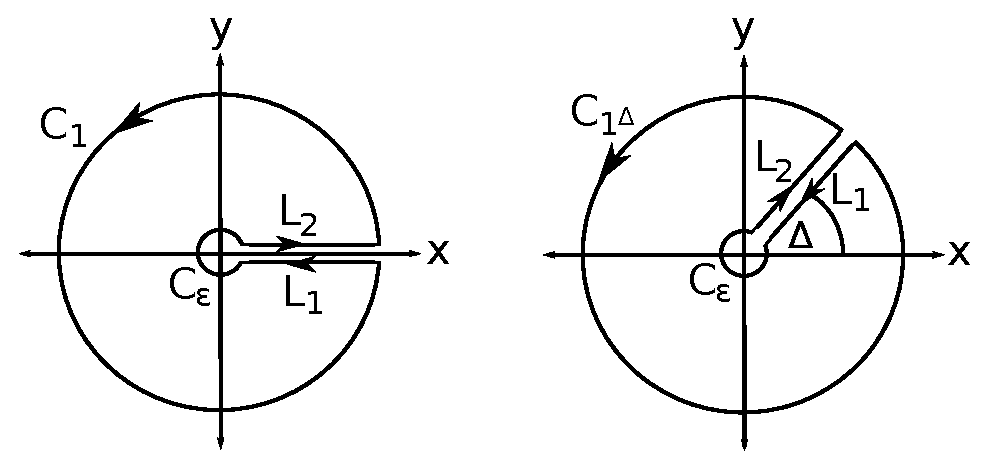
\includegraphics[scale=0.8]{branch-cut-plots/sq-root-cut.eps}
\end{center}
  \caption{\label{fig:sq-root-cut}
A choice of contour that includes a cut.}
\end{figure}
%

Branch cuts, what are they for? and how do we use them? For an illustration see Fig.~\ref{fig:sq-root-cut}. What we want to do here is to calculate $\oint_{C} \sqrt{z} dz$ along a unit circle around the origin. The tricky thing here is that $1 = e^{i0} = e^{i2\pi}$ but $\sqrt{1} \rightarrow e^{i0/2} \neq e^{i\pi}$! So we need to provide a cut such that the contour doesn't go full circle. First we will calculate $\oint_{C} \sqrt{z} dz$ using the contour shown in Fig.~\ref{fig:sq-root-cut} (left).
%
\nbea
\oint_{C} \sqrt{z} dz & = & \oint_{C_1} \sqrt{z} dz + \int_{L_1} \sqrt{z} dz + \oint_{C_\varepsilon} \sqrt{z} dz + \int_{L_2} \sqrt{z} dz \\
\rightarrow \oint_{C} \sqrt{z} dz & = & 0, ~~{\rm no~pole~inside~the~contour} \\
\rightarrow \oint_{C_1} \sqrt{z} dz & = & \int_{\varepsilon}^{2\pi - \varepsilon} \sqrt{1 e^{i\theta}} d\theta = \int_{0}^{2\pi} \sqrt{e^{i\theta}} d\theta = \oint_{C} \sqrt{z} dz \\ 
\rightarrow \int_{L_1} \sqrt{z} dz & = & \int_{1}^{\varepsilon} \sqrt{x e^{(2\pi - \varepsilon) i}} dx = \int_{1}^{0} \sqrt{x} e^{\pi i} dx = \int_{0}^{1} \sqrt{x}~ dx \\
\rightarrow \oint_{C_\varepsilon} \sqrt{z} dz & = & \int_{2\pi - \varepsilon}^{\varepsilon} \sqrt{\varepsilon e^{i \theta}} d\theta = 0 ~{\rm as}~\varepsilon \to 0 \\
\rightarrow \int_{L_2} \sqrt{z} dz & = & \int^{1}_{\varepsilon} \sqrt{x e^{\varepsilon i}} dx = \int^{1}_{0} \sqrt{x} ~dx 
\neea
%
and we take the limit of $\varepsilon \to 0$. Thus we have, after rearranging
%
\nbea
\oint_{C} \sqrt{z} dz & = & \oint_{C_1} \sqrt{z} dz + \int_{L_1} \sqrt{z} dz + \oint_{C_\varepsilon} \sqrt{z} dz + \int_{L_2} \sqrt{z} dz \\
\rightarrow 0 & = & \oint_{C} \sqrt{z} dz + \int_{0}^{1} \sqrt{x}~ dx + 0 + \int_{0}^{1} \sqrt{x}~ dx \\
\oint_{C} \sqrt{z} dz & = & - \int_{0}^{1} \sqrt{x}~ dx - \int_{0}^{1} \sqrt{x}~ dx \\
& = & -\frac{4}{3}
\neea
%
but what happens if we choose a cut that doesn't lie on the $x$ axis? say the cut is at an angle $\Delta$? as shown in Fig.~\ref{fig:sq-root-cut} (right), note that we want $L_1$ and $L_2$ to differ by $2\pi$ otherwise there's no point in introducing a cut, here $L_2$ is at angle $\Delta$ and $L_1$ is at angle $\Delta + 2\pi$
%
\nbea
\oint_{C^\Delta} \sqrt{z} dz & = & \oint_{C_{1^\Delta}} \sqrt{z} dz + \int_{L_{1^\Delta}} \sqrt{z} dz + \oint_{C_{\varepsilon^\Delta}} \sqrt{z} dz + \int_{L_{2^\Delta}} \sqrt{z} dz \\
\rightarrow \oint_{C^\Delta} \sqrt{z} dz & = & 0, ~~{\rm no~pole~inside~the~contour} \\
\rightarrow \oint_{C_{1^\Delta}} \sqrt{z} dz & = & \int_{\Delta + \varepsilon}^{\Delta + 2\pi - \varepsilon} \sqrt{1 e^{i\theta}} d\theta = \int_{\Delta}^{\Delta + 2\pi} \sqrt{e^{i\theta}} d\theta = \oint_{C^\Delta} \sqrt{z} dz \\ 
\rightarrow \int_{L_{1^\Delta}} \sqrt{z} dz & = & \int_{1}^{\varepsilon} \sqrt{r e^{(\Delta + 2\pi - \varepsilon) i}} dr = \int_{1}^{0} \sqrt{r} e^{i\Delta/2}e^{\pi i} dr = e^{i\Delta/2} \int_{0}^{1} \sqrt{r}~ dr \\
\rightarrow \oint_{C_{\varepsilon^\Delta}} \sqrt{z} dz & = & \int_{\Delta+2\pi - \varepsilon}^{\Delta+\varepsilon} \sqrt{\varepsilon e^{i \theta}} d\theta = 0 ~{\rm as}~\varepsilon \to 0 \\
\rightarrow \int_{L_{2^\Delta}} \sqrt{z} dz & = & \int^{1}_{\varepsilon} \sqrt{r e^{(\Delta+\varepsilon) i}} dr = e^{i\Delta/2} \int^{1}_{0} \sqrt{r} ~dr 
\neea
%
Now we have
%
\nbea
\oint_{C^\Delta} \sqrt{z} dz & = & \oint_{C_{1^\Delta}} \sqrt{z} dz + \int_{L_{1^\Delta}} \sqrt{z} dz + \oint_{C_{\varepsilon^\Delta}} \sqrt{z} dz + \int_{L_{2^\Delta}} \sqrt{z} dz \\
0 & = & \oint_{C^\Delta} \sqrt{z} dz + e^{i\Delta/2} \int_{0}^{1} \sqrt{r}~ dr + 0 + e^{i\Delta/2} \int^{1}_{0} \sqrt{r} ~dr \\
\oint_{C^\Delta} \sqrt{z} dz & = & -2 e^{i\Delta/2} \int_{0}^{1} \sqrt{r}~ dr \\
& = & e^{i\Delta/2} \left( -\frac{4}{3} \right )
\neea
%
So apparently we get a different result for different contours, but if we take a closer look
%
\nbea
\oint_{C^\Delta} \sqrt{z} dz & = & \int_{\Delta}^{\Delta + 2\pi} \sqrt{1 e^{i\theta}} d\theta \\
{\rm Let}~ \omega = \theta - \Delta & \rightarrow & d\omega = d\theta, ~ \int_{\Delta}^{\Delta + 2\pi} d\theta = \int_{0}^{2\pi} d\omega \\
\rightarrow \oint_{C^\Delta} \sqrt{z} dz & = & \int_{0}^{2\pi} \sqrt{1 e^{i(\omega + \Delta)}} d\omega \\
& = &  e^{i\Delta/2} \int_{0}^{2\pi} \sqrt{1 e^{i\omega}} d\omega \\
\oint_{C^\Delta} \sqrt{z} dz & = & e^{i\Delta/2} \oint_{C} \sqrt{z} dz
\neea
%
so indeed
%
\nbea
\oint_{C^\Delta} \sqrt{z} dz = e^{i\Delta/2} \oint_{C} \sqrt{z} dz & = & e^{i\Delta/2} \left( -\frac{4}{3} \right )\\
\rightarrow  \oint_{C} \sqrt{z} dz & = & -\frac{4}{3}
\neea
%
Thus rotating the branch cut (by an angle $\Delta$) does indeed rotate the original integral $\oint_{C} \sqrt{z} dz$ into $e^{i\Delta/2} \oint_{C} \sqrt{z} dz$, so we need to be careful.

A side note, how do we specify the contour if the circle is not at the origin but say is at $z_0$? Well, we can just parametrize the circle as $z = z_0 + r e^{i\theta}$ (remember that additions in the complex plane are vectorial operations), thus a contour integral of $z$ around a point $z_0$ is simply given by
%
\nbea
\oint z~dz \rightarrow \int_{0}^{2\pi} (z_0 + r e^{i\theta}) d\theta
\neea
%
%
\begin{figure}
\begin{center}
  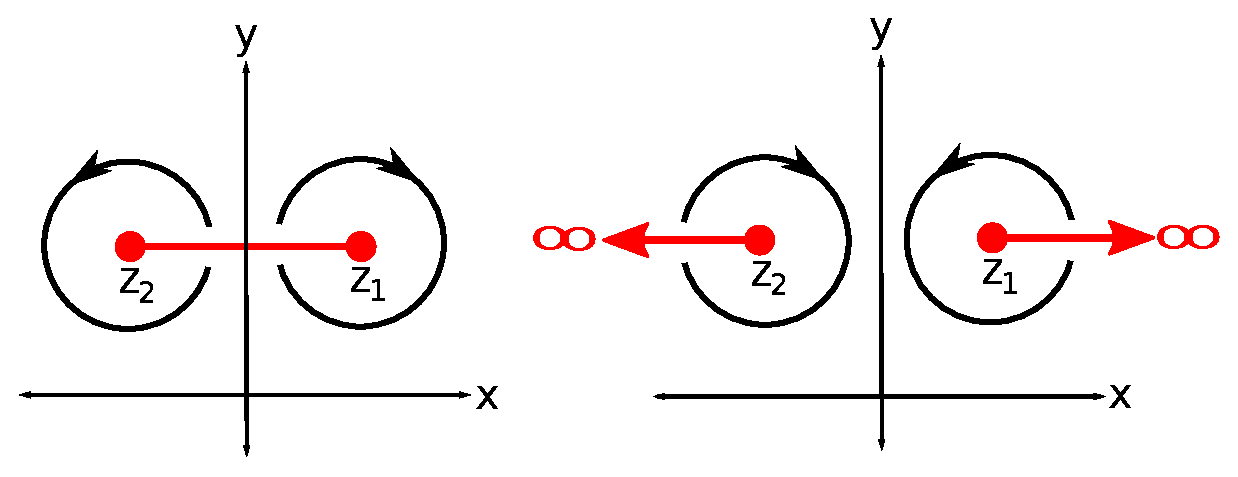
\includegraphics[scale=0.7]{branch-cut-plots/2-root-cut.eps}
\end{center}
  \caption{\label{fig:2-root-cut}
Different choices of contours that include a cut with 2 roots.}
\end{figure}
%
Going back to branch cuts, what if we have more than one root, \eg $\sqrt{(z-z_1)(z-z_2)}$? see Fig.~\ref{fig:2-root-cut}. Then there are two choices, we can put the cut between the roots as shown in Fig.~\ref{fig:2-root-cut} (left) or we can put the cuts starting from the roots to infinity as shown in Fig.~\ref{fig:2-root-cut} (right), the point here is to prevent a full circle around each root.

-=-=-=-=-=-=-=-=-=-=-=-=-=-=-=-=-=-=-=-=-=-=-=-=-=-=-=-=-

Throwback Tuesday! (today is Tuesday Oct 13 2015) High school favorite, how do we compute $\sin(18^\circ)$ without approximation and without a calculator? Well, start with $\sin(18^\circ) = \sin(90^\circ/5)$, since we know that $\sin(90^\circ) = 1$. However, our real starting point is actually $\cos(90^\circ/5)$ because $\cos(90^\circ) = 0$ and the end goal here is to transform $\sin(18^\circ)$ into solving a polynomial and it's easier to find the zeros of a polynomial if there's no constant.

First we need the formula for $\cos(5x)$. The easiest way to do this is to use Euler's formula
%
\nbea
e^{i5x} & = & \left ( e^{ix} \right ) ^5 \\
\rightarrow \cos(5x) + i \sin(5x) & = & \left ( \cos(x) + i \sin(x)\right )^5
\neea
%
In case you forget how to expand a polynomial, here's the Pascal's triangle
%
\nbea
& 1 & \\
1~~~ & 2 &~~~ 1 \\
1~~~ 3~ & &~ 3~~~ 1 \\
1~~~ 4~~~ & 6 &~~~ 4~~~ 1 \\
1~~~ 5~~~ 10 & & 10~~~ 5~~~ 1
\neea
%
the expansion is then
%
\nbea
\left ( \cos(x) + i \sin(x)\right )^5 & = & \cos^5(x) + 5 \cos^4(x)i\sin(x) + 10 \cos^3(x)i^2\sin^2(x) + \\
&& 10 \cos^2(x)i^3\sin^3(x) + 5 \cos(x)i^4\sin^4(x) + i^5\sin^5(x) \\
\rightarrow \cos(5x) & = & {\text {Re}} \left \{ \left ( \cos(x) + i \sin(x)\right )^5 \right \} \\
& = & \cos^5(x) - 10 \cos^3(x)\sin^2(x) + 5 \cos(x)\sin^4(x) \\
\rightarrow \sin(5x) & = & {\text {Im}} \left \{ \left ( \cos(x) + i \sin(x)\right )^5 \right \} \\
& = & 5 \cos^4(x)\sin(x) - 10 \cos^2(x)\sin^3(x) + \sin^5(x)
\neea
%
simplifying 
%
\nbea
\cos(5x) & = & \cos^5(x) - 10 \cos^3(x)\sin^2(x) + 5 \cos(x)\sin^4(x) \\
& = & \cos^5(x) - 10 \cos^3(x)(1 - \cos^2(x)) + 5 \cos(x)( 1 - \cos^2(x))^2 \\
& = & \cos^5(x) - 10 \cos^3(x) + 10 \cos^5(x) + 5 \cos(x)( 1 -2\cos^2(x) + \cos^4(x)) \\
& = & 11\cos^5(x) - 10 \cos^3(x) + 5 \cos(x) - 10\cos^3(x) + 5 \cos^5(x) \\
\cos(5x) & = & 16\cos^5(x) - 20 \cos^3(x) + 5 \cos(x)
\neea
%
while for $\sin$
%
\nbea
\sin(5x) & = & 5 \cos^4(x)\sin(x) - 10 \cos^2(x)\sin^3(x) + \sin^5(x) \\
& = & 5 (1 - \sin^2(x))^2 \sin(x) - 10 (1 - \sin^2(x))\sin^3(x) + \sin^5(x) \\
& = & 5 (1 - 2\sin^2(x) + \sin^4(x)) \sin(x) - 10 \sin^3(x) + 10 \sin^5(x) + \sin^5(x) \\
& = & 5 \sin(x) - 10\sin^3(x) + 5 \sin^5(x) - 10 \sin^3(x) + 11 \sin^5(x) \\
\sin(5x) & = & 16 \sin^5(x) - 20\sin^3(x) + 5 \sin(x)
\neea
%
We can of course derive the above result using the usual formulae, for example
%
\nbea
\sin(5x) & = & \sin(2x + 3x) \\
& = & \sin(2x)\cos(3x) + \cos(2x)\sin(3x) \\
\sin(2x) & = & 2\sin(x)\cos(x) \\
\cos(3x) & = & \cos(x + 2x) = \cos(x)\cos(2x) - \sin(x)\sin(2x) \\
\cos(2x) & = & \cos^2(x) - \sin^2(x) = 1 - 2\sin^2(x) \\
\sin(3x) & = & \sin(x + 2x) = \sin(x)\cos(2x) + \cos(x)\sin(2x)
\neea
%
and working out the algebra, the result will be the same. Now we see as to why starting out with $\sin(18^\circ) = \sin(90^\circ/5)$ doesn't work well
%
\nbea
 \sin(5 \times 18^\circ) = 1 & = & 16 \sin^5(18^\circ) - 20\sin^3(18^\circ) + 5 \sin(18^\circ) \\
1 & = & 16 \sin^5(18^\circ) - 20\sin^3(18^\circ) + 5 \sin(18^\circ)
\neea
%
the LHS is not zero, while starting with $\cos(18^\circ) = \cos(90^\circ/5)$ does work
%
\nbea
 \cos(5 \times 18^\circ) = 0 & = & 16 \cos^5(18^\circ) - 20\cos^3(18^\circ) + 5 \cos(18^\circ) \\
0 & = & \cos(18^\circ) (16\cos^4(18^\circ)  - 20\cos^2(18^\circ) + 5), ~~ {\rm Let~} x = \cos^2(18^\circ) \\
0 & = & 16x^2 - 20x + 5  \\
x & = & \frac{20 \pm \sqrt{400 - 320} }{32} = \frac{20 \pm 4\sqrt{5} }{32}
\neea
%
we just need to take the $+$ of the $\pm$ since $\cos$ of small angles are closer to one. The result we want is then given by
%
\nbea
\sin(18^\circ) & = & \sqrt{\sin^2(18^\circ)} = \sqrt{1- \cos^2(18^\circ)} = \sqrt{1 - x} \\
& = &\sqrt{ 1 - \frac{20 + 4\sqrt{5} }{32}} \\
\sin(18^\circ) & = & \sqrt{ \frac{3 - \sqrt{5} }{8} }
\neea
%
but wait, how do you calculate the square root by hand? The problem states that we should calculate it without a calculator. 

To calculate square roots by hand we use the ubiquitous formula $(a + b)^2 = a^2 + 2ab + b^2$ and do it iteratively. Say we want to find the root of a number, \eg $\sqrt{C}$, first we do a rough approximation $C_1^2 < C$ and then we find the next factor $C_2$ through
%
\nbea
C & = & (C_1 + C_2)^2 = C_1^2 + 2C_1C_2 + C_2^2 \\
(C - C_1^2) & = & (2C_1 + C_2)C_2
\neea
%
finding the largest $C_2$ such that $(2C_1 + C_2)C_2 < (C - C_1^2)$. Once we find $C_2$ we repeat the process
%
\nbea
C & = & (\{C_1 + C_2\} + C_3)^2 = \{C_1 + C_2\}^2 + 2\{C_1 + C_2\}C_3 + C_3^2 \\
(C - \{C_1 + C_2\}^2) & = & (2\{C_1 + C_2\} + C_3)C_3
\neea
%
by finding the largest $C_3$ such that $(2\{C_1 + C_2\} + C_3)C_3 < (C - \{C_1 + C_2\}^2)$. In other words
%
\nbea
C_1 & \rightarrow & {\rm largest~number~such~that~}C_1^2 < C\\
C_n & \rightarrow & {\rm largest~number~such~that~}\left ( 2\left ( \sum_{i=1}^{n-1} C_i \right ) + C_n \right ) C_n < \left ( C - \left ( \sum_{i=1}^{n-1} C_i \right )^2 \right ) \\
\rightarrow \sqrt{C} & = & \sum_{i=1}^{\infty} C_i
\neea
%
You can stop anytime you want, depending on the accuracy you need. The above prescription is correct but we want to make it more systematic by dividing the number into `hundreds', partitioning it into 2-digit groupings (hundreds because our digits run from $0$ to $9$ which translate to $0$ to $<100$). Let's see how it works with a concrete example

{\renewcommand{\arraystretch}{0.2} %<- modify value to suit your needs
\begin{tabular}{r l}
 & ~~~~2~~3~~8.~~~3~ ~0~~4~~4 \\
 & $\sqrt{~5~67~89.~01~20~00~00}$ \\
 $2 \times 2 =$ & ~~~~4\\
 & ~~~--------------------------- - \\
 & ~~~~1~67 \\
 $((2) (10) (2) + 3) \times 3= $ & ~~~~1~29\\
 & ~~~--------------------------- - \\
 &~~~~~~38~89 \\
 $((2) (10) (23) + 8) \times 8= $ & ~~~~~~37~44\\
  & ~~~--------------------------- - \\
 & ~~~~~~~~1~45~01\\
 $((2) (10) (238) + 3) \times 3= $ & ~~~~~~~~1~42~89\\
 & ~~~--------------------------- - \\
 & ~~~~~~~~~~~~2~12~20\\
 $((2)(10)(2383) + 0) \times 0= $ & ~~~~~~~~~~~~0~00~00\\
 & ~~~--------------------------- - \\
 &~~~~~~~~~~~~2~12~20~00\\
 $((2)(10)(23830) + 4) \times 4= $ &~~~~~~~~~~~~1~90~64~16\\
 & ~~~--------------------------- - \\
 &~~~~~~~~~~~~~~~21~55~84~00\\
 $((2)(10)(238304) + 4) \times 4= $ &~~~~~~~~~~~~~~~19~06~43~36\\\\\\
\end{tabular}
}

Thus $\sqrt{56789.012} = 238.3044 ...$

What we need to take note above is that $C_1$ takes care only the first digit, this makes it a lot easier to start the procedure, rather than trying to figure out 238 from the start.

In the second iteration, we multiply $C_1$ by 10 and at the same time `multiplying' the target by 100 by including the next 2 digits as
%
\nbea
100C & = & 100(C_1 + C_2)^2 = 100 C_1^2 + 200C_1C_2 + 100 C_2^2 \\
100(C - C_1^2) & = & (2 (10) C_1 + C_2) C_2
\neea
%
Another important point is that $C_5=0$! Zero is apparently permitted. I actually learned this method when I was 10 but didn't understand the reasoning behind it.

Another way of computing square roots is using taylor expansion
%
\nbea
\sqrt{1 + x} & = & 1 + \frac{1}{2} x + \sum^{\infty}_{n=1} \frac{(-1)^n (2n-1)!!}{2^n} x^{n+1}
\neea
%
for example
%
\nbea
\sqrt{101} = 10\sqrt{1 + 0.01} & = & 10 \left (1 + \frac{1}{2} (0.01) - \frac{1}{2} (0.01)^{2} + \frac{(1) (3)}{2^2} (0.01)^{3} + ... \right )
\neea
%
but the convergence might be slow due to the alternating signs in the series. One important note here is that although the previous method looks a lot like the usual division algorithm, they are extremely different. In the case of roots, you need to keep using the previous results to compute the next one, not so with divisions, this is because divisions are linear while roots are not.

-=-=-=-=-=-=-=-=-=-=-=-=-=-=-=-=-=-=-=-=-=-=-=-=-=-=-=-=-

Why does a number that is a multiple of 9 have digits tham sum up to be a multiple of 9? \eg
%
\nbea
3 \times 9 = 27 & \rightarrow & 2 + 7 = 9 \\
13 \times 9 = 117 & \rightarrow & 1 + 1 + 7 = 9 \\
5555 \times 9 = 49995 & \rightarrow & 4 + 9 + 9 + 9 + 5 = 36 = 4 \times 9
\neea
%
First of all, any number can be written as
%
\nbea
a_Na_{N-1}a_{N-2}...a_2a_1a_0 & = & \sum_{i = 0}^{N} a_i 10^i, ~~a_i \in \{0,1,2,3,4,5,6,7,8,9\}
\neea
%
\eg 10937 $\to a_4 = 1, a_3 = 0, a_2 = 9, a_1 = 3, a_0 = 7$, now say we have a number that is a multiple of 9, $b = 9 n$, with $n$ a positive integer
%
\nbea
b = 9 n & = & \sum_{i = 0}^{N} a_i 10^i \\
\sum_{i = 0}^{N} a_i 10^i & = & \sum_{i = 1}^{N} a_i (10^i - 1) + \sum_{i = 0}^{N} a_i
\neea
%
but we can rewrite
%
\nbea
\left (10^i - 1 \right ) & = & \sum_{j = 0}^{i-1} 9(10)^j = 9\sum_{j = 0}^{i-1} (10)^j \\
\rightarrow \sum_{i = 0}^{N} a_i 10^i & = & \sum_{i = 1}^{N} a_i \left (9 \sum_{j = 0}^{i-1} (10)^j \right ) + \sum_{i = 0}^{N} a_i \\
b = 9n & = & 9 \left ( \sum_{i = 1}^{N} a_i \left ( \sum_{j = 0}^{i-1} (10)^j \right ) \right ) + \sum_{i = 0}^{N} a_i \\
9 n - 9 \left ( \sum_{i = 1}^{N} a_i \left ( \sum_{j = 0}^{i-1} (10)^j \right ) \right ) & = & \sum_{i = 0}^{N} a_i \\
\neea
%
Thus the sum of the digits $\sum_{i = 0}^{N} a_i = 9m$ is a multiple of nine, \eg 41076 = $9 \times 4654$
%
\nbea
9 \times 4654 = 41076 & = & 4 \times 10000 + 1 \times 1000 + 0 \times 100 + 7 \times 10 + 6 \\
& = & (4 \times (10000-1) + 1 \times (1000-1) + 0 \times (100-1) + 7 \times (10-1)) + \\
&&  ( 4 + 1 + 0 + 7 + 6) \\
& = & (4 \times 9999 + 1 \times 999 + 0 \times 99 + 7 \times 9) + ( 4 + 1 + 0 + 7 + 6) \\
9 \times 4654 & = & 9 \times (4 \times 1111 + 1 \times 111 + 0 \times 11 + 7 \times 1) + ( 4 + 1 + 0 + 7 + 6)
\neea
%
Hence $ ( 4 + 1 + 0 + 7 + 6)$ must be a multiple of 9.

Note that the above argument is also valid for multiples of 3, \ie digits of a number that is a multiple of 3 sum up to a multiple of 3.

-=-=-=-=-=-=-=-=-=-=-=-=-=-=-=-=-=-=-=-=-=-=-=-=-=-=-=-=-

%
\begin{figure}
\begin{center}
  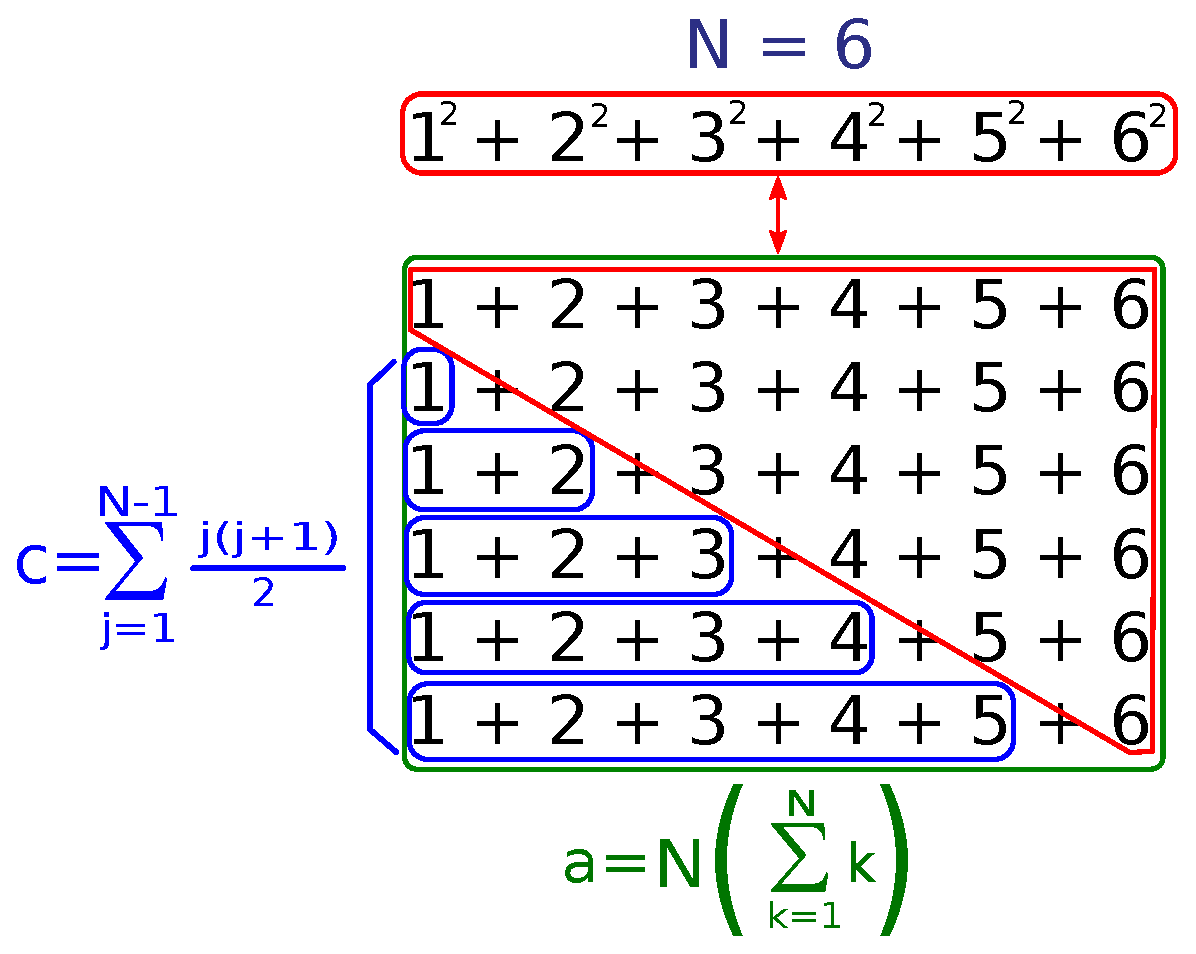
\includegraphics[scale=0.45]{n-squared-plots/n_squared_sum_box_1.eps}
\end{center}
  \caption{\label{fig:sum-sq-1}
An illustration on how to calculate sum of squares.}
\end{figure}
%
What is the explicit formula for $\sum_{i=1}^{N} i^2$? I saw this on the bus on my way to work a long time ago, took me a day to finally figure it out. You can say that we can use induction to prove the formula however, induction only allows you to prove what you already know {\it not} to derive the formula itself in the first place! {\it inductio no ex nihilo} :)

The easiest way to derive the formula for $\sum_{i=1}^{N} i^2$ is to actually draw it, see Fig.~\ref{fig:sum-sq-1}. The series we want to sum is shown in the top red box, \ie $\sum_{i=1}^{N=6} i^2 = 1^2 + 2^2 + 3^2 + 4^2 + 5^2 + 6^2$.

This sum $\sum_{i=1}^{N=6} i^2$ is also represented by the upper red triangle in Fig.~\ref{fig:sum-sq-1} because that is the definition of squares, \eg $2^2 = 2 + 2,~3^2 = 3 + 3 + 3$. However, Fig.~\ref{fig:sum-sq-1} also shows how we can calculate this upper red triangle, it is nothing but the sum in the green box $a$ minus the sum in the lower blue triangle $c$.

The sum in the green box is given by $a = 6 \times (1 + 2 + 3 + 4 + 5 +6) = N\sum_{k=1}^{N=6} k$, the lower blue triangle is given by $c= \sum^{N-1}_{j=1} \sum_{m=1}^{j} m = \sum^{N-1}_{j=1} j(j+1)/2$, where we have used the famous gauss formula for $\sum_{m=1}^{N} m = N(N+1)/2$.

The sum $\sum_{i=1}^{N} i^2$ is then given by
%
\nbea
\sum_{i=1}^{N} i^2 & = & a - c \\
& = & \left ( N\sum_{k=1}^{N} k \right ) - \left ( \sum^{N-1}_{j=1} \frac{j(j+1)}{2} \right ) \\
& = & \left ( N \frac{N(N+1)}{2}\right ) - \left ( \frac{1}{2} \sum^{N-1}_{j=1} j^2 + \frac{1}{2} \sum^{N-1}_{j=1} j \right ) \\
\sum_{i=1}^{N} i^2 & = & \left ( N \frac{N(N+1)}{2}\right ) - \left ( \left \{ \frac{1}{2} \sum^{N}_{j=1} j^2 - \frac{1}{2} N^2 \right \} + \frac{1}{2} \sum^{N-1}_{j=1} j \right ) \\
\sum_{i=1}^{N} i^2 +  \frac{1}{2} \sum^{N}_{j=1} j^2 & = & \left ( \frac{N^3 + N^2}{2}\right ) - \left ( - \frac{1}{2} N^2 + \frac{1}{2} \frac{(N-1)N}{2} \right ) \\
& = & \frac{N^3 + N^2}{2} + \frac{1}{2} N^2 -  \frac{(N-1)N}{4} \\
\frac{3}{2} \sum^{N}_{i=1} i^2 & = &  \frac{2N^3 + 2N^2 + 2N^2 - N^2 + N}{4} \\
& = & \frac{2N^3 + 3N^2 + N}{4} = \frac{N(N+1)(2N+1)}{4} \\
\rightarrow \sum^{N}_{i=1} i^2 & = & \frac{N(N+1)(2N+1)}{6}
\neea
%
And that is the formula we are after!

Bonus !!!

We can use the above result to calculate $c$ explicitly in terms of $N$
%
\nbea
c & \equiv & \sum^{N}_{j=1} \frac{j(j+1)}{2} = \frac{1}{2} \sum^{N}_{j=1} j^2 + \frac{1}{2} \sum^{N}_{j=1} j \\
& = & \frac{1}{2} \frac{2N^3 + 3N^2 + N}{6} + \frac{1}{2}\frac{N^2 + N}{2} \\
& = & \frac{2N^3 + 6N^2 + 4N}{12} = \frac{N^3 + 3N^2 + 2N}{6} \\
\sum^{N}_{j=1} \frac{j(j+1)}{2} & = & \frac{N^3 + 3N^2 + 2N}{6}
\neea
%
Now, we can use this result to get something interesting. Note that the blue lower triangle $c$ in Fig.~\ref{fig:sum-sq-1} can be seen as a sum in the vertical direction, \ie
%
\nbea
c & = & 1(5) + 2(4) + 3(3) + 4(2) + 5(1) \\
& = & 1(5 - 0) + 2(5 - 1) + 3(5 - 2) + 4(5 - 3) + 5(5 - 4) \\
& = & 5 (1 + 2 + 3 + 4 + 5) - (2(1) + 3(3) + 4(2) + 5(1)) \\
\frac{N^3 + 3N^2 + 2N}{6} & = & \left ( N\sum_{i=1}^{N} i \right ) - \sum_{i=2}^{N} i(i-1), ~~N=5
\neea
%
where in the last line we have used the explicit formula for $c$. Switching sides and generalizing to any $N$
%
\nbea
\sum_{i=2}^{N} i(i-1) & = & \left ( N\sum_{i=1}^{N} i \right ) - \frac{N^3 + 3N^2 + 2N}{6} \\
& = & \frac{N^3 + N^2}{2} - \frac{N^3 + 3N^2 + 2N}{6} \\
& = & \frac{3N^3 + 3N^2 - N^3 - 3N^2 - 2N}{6} \\
& = & \frac{2N^3 - 2N}{6} \\
\sum_{i=2}^{N} i(i-1) & = & \frac{N^3 - N}{3}
\neea
%
We can now in turn use this result to calculate $1 + 2(1) + 3(2) + 4(3) + ... + N(N-1)$, \ie
%
\nbea
1 + \sum_{i=2}^{N} i(i-1) = 1 + \sum_{i=2}^{N} \frac{i!}{(i-2)!} = \frac{N^3 - N}{3} + 1
\neea
%
Looking back at how we calculated $\sum_{i=1}^{N} i^2$ using Fig.~\ref{fig:sum-sq-1}, we can easily generalize it to calculate $\sum_{i=1}^{N} i^k, k > 2$, see Fig.~\ref{fig:sum-sq-2}. To simplify things let's designate $f_k(N) \equiv \sum_{i=1}^{N} i^k$ as the sum of $k$-th powers.
%
\begin{figure}
\begin{center}
  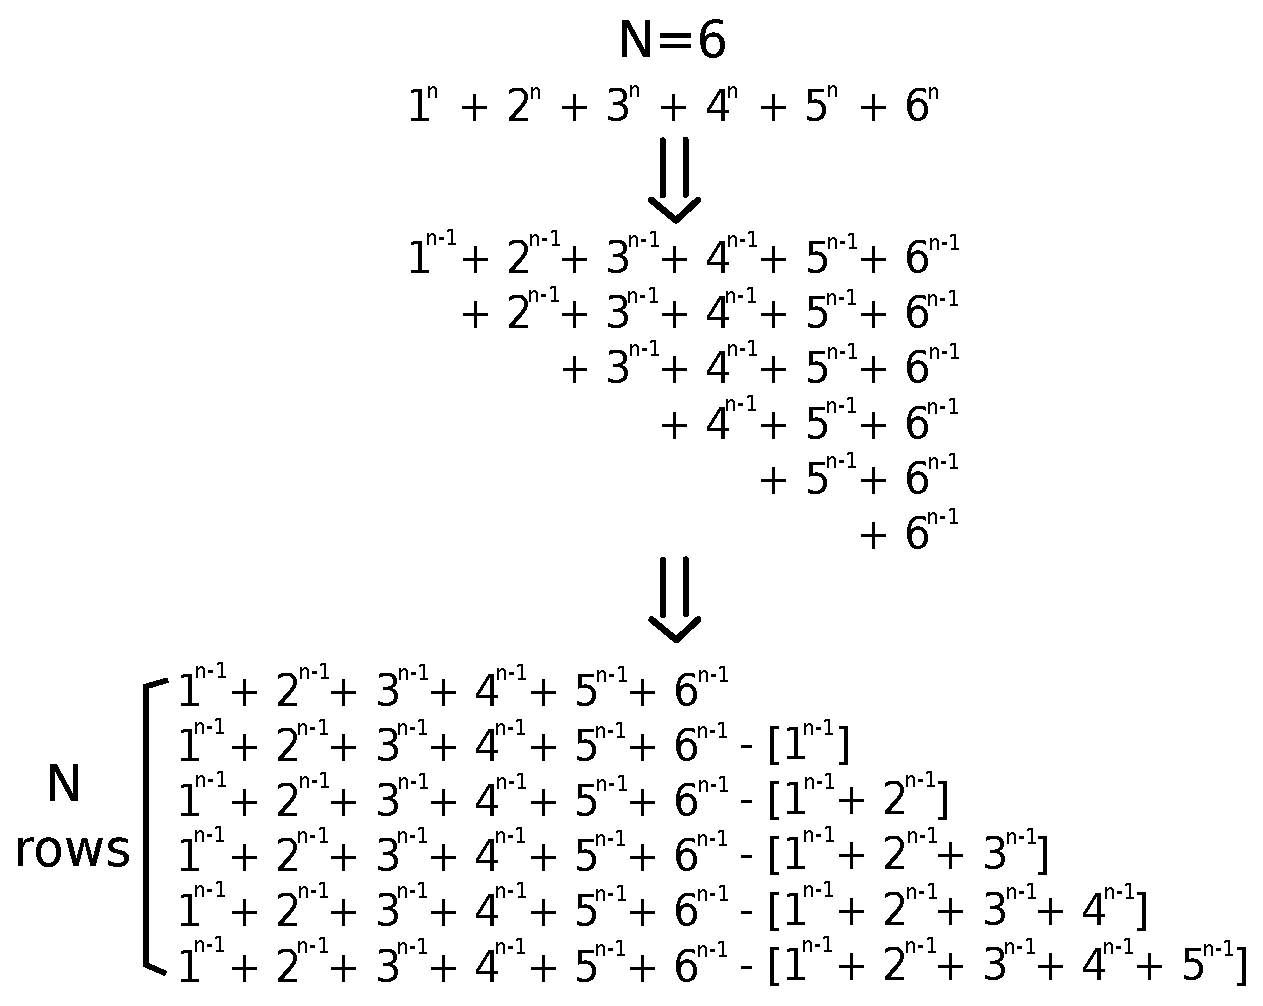
\includegraphics[scale=0.55]{n-squared-plots/n_squared_sum_box_2.eps}
\end{center}
  \caption{\label{fig:sum-sq-2}
An illustration on how to calculate sum of $n$-th powers.}
\end{figure}
%

From Fig.~\ref{fig:sum-sq-2} it's immediately apparent that we can calculate $f_k(N)$ through
%
\nbea
f_k(N) & = & N f_{k-1}(N) - \sum_{m=1}^{N-1} f_{k-1}(m) \\
& = & N f_{k-1}(N) - \left ( \sum_{m=1}^{N} f_{k-1}(m)  - f_{k-1}(N) \right ) \\
f_k(N) & = & (N+1) f_{k-1}(N) - \sum_{m=1}^{N} f_{k-1}(m)
\neea
%
which is a recursion relation for the sum of any $k$-th powers.

Let's see a concrete example by calculating $f_3(N) = \sum_{i=1}^{N} i^3$
%
\nbea
f_3(N) & = & (N+1) f_{2}(N) - \sum_{m=1}^{N} f_{2}(m) \\
& = & (N+1) \frac{2N^3 + 3N^2 + N}{6} - \sum_{m=1}^{N} \frac{2m^3 + 3m^2 + m}{6} \\
\sum_{i=1}^{N} i^3 + \frac{2}{6} \sum_{m=1}^{N} m^3 & = &  \frac{2N^4 + 5N^3 + 4N^2 + N}{6} - \frac{2N^3 + 3N^2 + N}{12} - \frac{N^2 + N}{12} \\
\frac{4}{3}\sum_{i=1}^{N} i^3 & = & \frac{4N^4 + 8N^3 + 4N^2}{12} \\
& = & \frac{N^4 + 2N^3 + N^2}{3} = \frac{N^2(N + 1)^2}{3} \\
\rightarrow \sum_{i=1}^{N} i^3 & = & \frac{N^2(N + 1)^2}{4}
\neea
%
so {\it theoretically} we can compute the explicit formula for the sum of any $k$-th power using
%
\nbea
f_k(N) & = & (N+1) f_{k-1}(N) - \sum_{m=1}^{N} f_{k-1}(m)
\neea
%
(with $f_0(N) = \sum_{i=1}^{N} 1 = N$) which is the gist of the algorithm. The following list shows $f_k(N)$ up to $k=15$ when the expression starts becoming unwieldy, but there's a pattern, the even $k$ starts with $N(N+1)(2N+1)$ while the odd $k$ starts with $N^2(N+1)^2$.
{
\begin{tabular}{ c l l }
$f_0$ &= $N$ & \\
$f_1$ &= $\frac{N^2 + N}{2}$ &= $\frac{N(N+1)}{2}$ \\
$f_2$ &= $\frac{2N^3 + 3N^2+ N}{6}$ &= $\frac{N(N+1)(2N+1)}{6}$ \\
$f_3$ &= $\frac{N^4 + 2N^2+ N}{4}$ &= $\frac{N^2(N+1)^2}{4}$ \\
$f_4$ &= $\frac{6N^5 + 15N^4 + 10N^3 - N}{30}$ &= $\frac{N(N+1)(2N+1)(3N^2 + 3N - 1)}{30}$ \\
$f_5$ &= $\frac{2N^6 + 6N^5 + 5N^4 - N^2}{12}$ &= $\frac{N^2(N+1)^2(2N^2 + 2N - 1)}{12}$ \\
$f_6$ &= $\frac{6N^7 + 21N^6 + 21N^5 - 7N^3 + N}{42}$ &= $\frac{N(N+1)(2N+1)(3N^4 + 6N^3 - 3N + 1)}{42}$ \\
$f_7$ &= $\frac{3N^8 + 12N^7 + 14N^6 - 7N^4 + 2N^2}{24}$ &= $\frac{N^2(N+1)^2(3N^4 + 6N^3 - N^2 - 4N + 2)}{24}$ \\
$f_8$ &= $\frac{10N^9 + 45N^8 + 60N^7 -42N^5 + 20N^3 - 3N}{90}$ &= $\frac{N(N+1)(2N+1)(5N^6 + 15N^5 + 5N^4 - 15N^3 - N^2 + 9N - 3)}{90}$ \\
$f_9$ &= $\frac{2N^{10} + 10N^9 + 15N^8 - 14N^6 + 10N^4 - 3N^2}{20}$ &= $\frac{N^2(N+1)^2(N^2 + N - 1)(2N^4 + 4N^3 - N^2 - 3N + 3)}{20}$ \\
$f_{10}$ &= $\frac{6N^{11} + 33N^{10} + 55N^9 - 66N^7 + 66N^5 - 33N^3 + 5N}{66}$ &= $\frac{N(N+1)(2N+1)(N^2 + N - 1)(3N^6 + 9N^5 + 2N^4 - 11N^3 + 3N^2 + 10N - 5)}{66}$ \\
$f_{11}$ &= $\frac{2N^{12} + 12N^{11} + 22N^{10} - 33N^8 + 44N^6 - 33N^4 + 10N^2}{24}$ &= $\frac{N^2(N+1)^2(2N^8 + 8N^7 + 4N^6 - 16N^5 -5N^4 + 26N^3 - 3N^2 - 20N +10)}{24}$
\end{tabular}
}
{
\begin{tabular}{ c l }
$f_{12}$ &= $\frac{210N^{13} + 1365N^{12} + 2730N^{11} - 5005N^9 + 8580 N^7 - 9009N^5 + 4550N^3 - 691N}{2730}$ \\
&= $\frac{N(N+1)(2N+1)(105N^{10} + 525N^9 - 1050N^7 - 1190N^6 + 2310 N^5 + 1420 N^4 - 3285 N^3 - 287N^2 + 2073N - 691)}{2730}$ \\
$f_{13}$ &= $\frac{30N^{14} + 210N^{13} + 455N^{12} - 1001N^{10} + 2145 N^8 - 3003N^6 + 2275N^4 - 691N^2}{420}$ \\
&= $\frac{N^2(N+1)^2(30N^{10} + 150N^9 - 400N^7 - 326N^6 + 1052 N^5 + 367 N^4 - 1786 N^3 - 202N^2 + 1382N - 691)}{420}$ \\
$f_{14}$ &= $\frac{6N^{15} + 45N^{14} + 105N^{13} - 273N^{11} + 715 N^9 - 1287N^7 + 1365N^5 - 691N^3 + 105N}{90}$ \\
&= $\frac{N(N+1)(2N+1)(3N^{12} + 18N^{11} + 24N^{10} - 45N^9 - 81N^8 + 144N^7 + 182N^6 - 345 N^5 - 217 N^4 + 498 N^3 + 44N^2 - 315N +105)}{90}$ \\
$f_{15}$ &= $\frac{3N^{16} + 24N^{15} + 60N^{14} - 182N^{12} + 572N^{10} - 1287N^8 + 1820 N^6 - 1382N^4 + 420N^2}{48}$ \\
&= $\frac{N^2(N+1)^2(3N^{12} + 18N^{11} + 21N^{10} - 60N^9 - 83N^8 +226N^7 + 203N^6 - 632N^5 -226N^4 +1084N^3 - 122N^2 -840N +420)}{48}$
\end{tabular}
}

The above list was generated using maxima with a small C code to generate the maxima script. The algorithm is quite simple as can be seen from our calculation of $f_3(N)$ above. To compute $f_k$ we need the coefficient of each $N^p$ in $f_{k-1}(N)$, note that $f_m(N)$ is a polynomial of order $N^{m+1}$. That is
%
\nbea
f_{k-1}(N) & = & \sum_{p=0}^{k} C^{(k-1)}_{p} N^p
\neea
%
The superscript in $ C^{(k-1)}_{p}$ indicates which $f_{k-1}$ this coefficient belongs to. We then have
%
\nbea
f_k & = & (N+1)f_{k-1} - \sum_{m=1}^{N} f_{k-1}(m) \\
& = & (N+1)f_{k-1} - \sum_{m=1}^{N} \sum_{p=0}^{k} C^{(k-1)}_p m^p \\
& = & (N+1)f_{k-1} - \sum_{p=0}^{k} \left (C^{(k-1)}_p \times \sum_{m=1}^{N} m^p \right ) \\
& = & (N+1)f_{k-1} - \sum_{p=0}^{k} \left (C^{(k-1)}_p f_p \right ) \\
f_k & = & (N+1)f_{k-1} - C^{(k-1)}_k f_k - \sum_{p=0}^{k-1} C^{(k-1)}_p f_p \\
f_k + C^{(k-1)}_k f_k & = & (N+1)f_{k-1} - \sum_{p=0}^{k-1} C^{(k-1)}_p f_p \\
\rightarrow f_k & = & \frac{1}{\left ( 1 + C^{(k-1)}_k \right )} \times \left ( (N+1)f_{k-1} - \sum_{p=0}^{k-1} C^{(k-1)}_p f_p \right ) \\
\neea
%
The moral of the story here is that although Gauss's method (adding the first and last number and second and second last and so on) works for $\sum i$ it doesn't work for any other power of $i^n$. A blessing and a curse, I don't know what's worse :)

-=-=-=-=-=-=-=-=-=-=-=-=-=-=-=-=-=-=-=-=-=-=-=-=-=-=-=-=-

Now on to something fun :)

Here's the proof that 1 is equal to any number $n$
%
\nbea
a & = & b \\
a b^{n-1} & = & b^{n}\\
a^{n-1} b & = & b^{n}\\
a^{n-1} b - a^{n} & = & b^{n} - a^{n}\\
a^{n-1} \cancel{(b - a)} & = & \cancel{(b - a)} \sum_{i=1}^{n} b^{n-i} a^{i-1} \\
a^{n-1} & = & \sum_{i=1}^{ n} a^{n-i} a^{i-1} \\
\cancel{a^{n-1}} & = &  n ~ \cancel{a^{n-1}} \\
1 & = & n
\neea
%
In case you forget how to factor $b^{n} - a^{n} = (b - a) \sum_{i=1}^{n} b^{n-i} a^{i-1}$, you start by pulling out the factors one at a time
%
\nbea
b^{n}  -  a^{n} & = & (b  -  a) (b^{n-1} + ... \\
\rightarrow - a) (b^{n-1} & = & - b^{n-1} a
\neea
%
so you need to add $(b^{n-1} + b^{n-2} a ... \rightarrow (b  b^{n-2} a)$ to cancel $-  a) (b^{n-1} = - b^{n-1} a$ introduced by the first factor $(b^{n-1} + ...$, but then again you generate $- a) (b^{n-2} a = -b^{n-2} a^2$ so you repeat the process until you get
%
\nbea
b^{n}  -  a^{n} & = & (b  -  a) (b^{n-1} + b^{n-2} a + b^{n-3} a^2 + ... + b a^{n-2} + a^{n-1})
\neea
%

-=-=-=-=-=-=-=-=-=-=-=-=-=-=-=-=-=-=-=-=-=-=-=-=-=-=-=-=-

\bigskip\underline{\textit{\textbf{A stroll with Monsieur Fermat}}}

The most annoying thing about Fermat's last theorem is that it looks so simple. Proving it however, was almost impossible even for the greatest mathematical minds that ever walked this planet. So what am I doing here? Let's see.

One might be tempted to think that going from a pythogorean equation with power of two to a cubic one is trivial, after all $3 = 2 + O(1)$ :) As an illustration, remember the quadratic formula? We can all derive it in five minutes or less, what it does is nothing but completing the square. Not so with the cubic formula, we can't just complete the cube. The solution to a cubic equation is in general a cube root of a square root in the form of $(a + (b^{1/2}))^{1/3}$. Yup the roots are nested. It's not as intuitive as I thought.

\bigskip\textbf{\textit{Prolegomenon: some greek sounding word for ``Introduction''}}

So of course I'm not going to even try proving Fermat, what I'm doing here is to see if there's anything I can learn from it.

We start this discussion with something more obvious and lots of doodles :) The great divide for $n \le 2$ and $n \ge 3$ can be seen immediately from the plot $x^n + y^n = 1$. Let's start with $x^1 + y^1 = 1$ which is a straight line, Fig.~\ref{fig:n_1}, bumping it into $x^3 + y^3 = 1$ adds a little ``bump'' to that straight line, Fig.~\ref{fig:n_3}, while increasing the power to $115$ makes that bump a lot sharper, Fig.~\ref{fig:n_115}.
%
\begin{figure}
\centering
\begin{subfigure}{.33\textwidth}
  \centering
  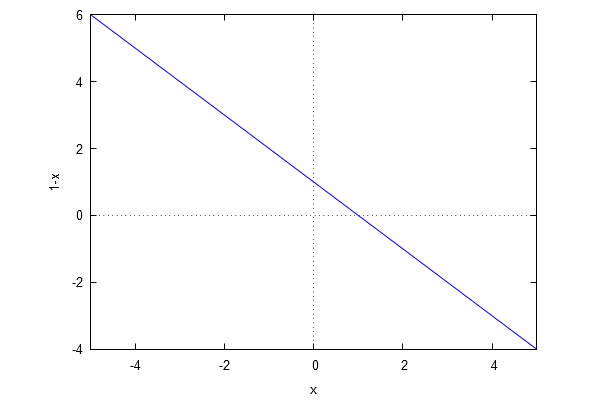
\includegraphics[width=1.1\linewidth]{FLT_n_1.png}
  \caption{Plot for $x^1 + y^1 = 1$}
  \label{fig:n_1}
\end{subfigure}%
\begin{subfigure}{.33\textwidth}
  \centering
  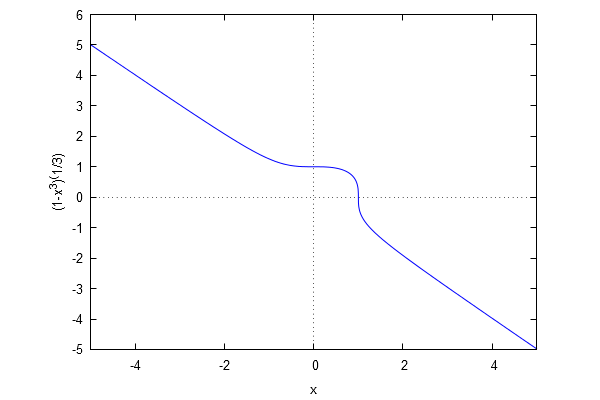
\includegraphics[width=1.1\linewidth]{FLT_n_3.png}
  \caption{Plot for $x^3 + y^3 = 1$}
  \label{fig:n_3}
\end{subfigure}
\begin{subfigure}{.33\textwidth}
  \centering
  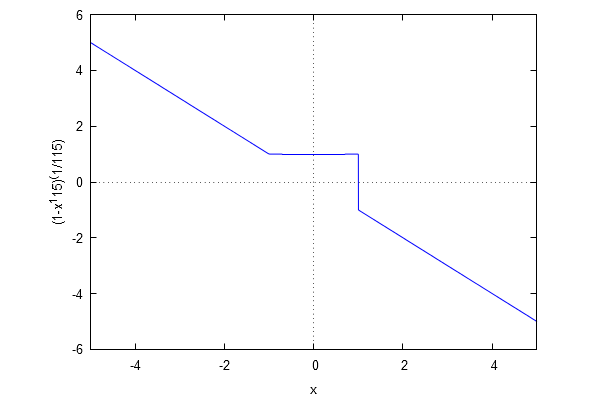
\includegraphics[width=1.1\linewidth]{FLT_n_115.png}
  \caption{Plot for $x^{115} + y^{115} = 1$}
  \label{fig:n_115}
\end{subfigure}
\caption{The higher the power the sharper the bump. For all three plots, vertical axis is $y$ and horizontal axis is $x$.}
\label{fig:FLT_n_odd}
\end{figure}
%

But that's not the only great division, even powers have all the same shape (which is different from the odd one), Fig.~\ref{fig:n_4}, except that the corners get sharper the higher the power, Fig.~\ref{fig:n_12}. The only exception to this is the Pythagorean equation $x^2 + y^2 = 1$ which is a circle and the only plot with maximum symmetry among $x^n + y^n = 1$.

One interesting thing here (thanks to Wildberger) is whether those curves actually exist, \eg for $x^3 + y^3 = 1$ the only rational solution is $(1,0), (0,1)$ this means that all other points on the curve are real numbers, however, the curves in Fig.~\ref{fig:n_3}, \ref{fig:n_115}, \ref{fig:FLT_n_even} are calculated by a computer program and we all know that computers can {\it not} process real numbers.

This seems to suggest that there is something special about Pythagoras, looks like ``no. 2" is actually number 1 :)
%
\begin{figure}
\centering
\begin{subfigure}{.5\textwidth}
  \centering
  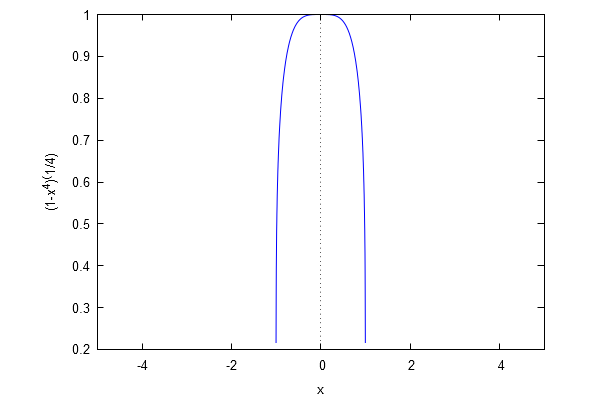
\includegraphics[width=1.1\linewidth]{FLT_n_4.png}
  \caption{Plot for $x^4 + y^4 = 1$}
  \label{fig:n_4}
\end{subfigure}%
\begin{subfigure}{.5\textwidth}
  \centering
  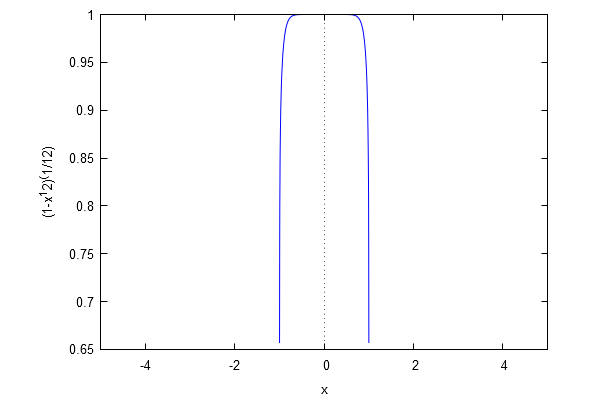
\includegraphics[width=1.1\linewidth]{FLT_n_12.png}
  \caption{Plot for $x^{12} + y^{12} = 1$}
  \label{fig:n_12}
\end{subfigure}
\caption{Sharper corners for sharper powers. For both plots, vertical axis is $y$ and horizontal axis is $x$.}
\label{fig:FLT_n_even}
\end{figure}
%

\bigskip\textbf{\textit{Idea \#1}}

Thanks to Wildberger's youtube videos the following ideas poped up in my head. The ancient greeks didn't use numbers like we do today, what we use are actually the arabic numerals. The greeks used line segments. To add one line segment on another you just join the two line segments to get a longer one. So I was curious as to what geometric meaning Fermat's last theorem presents us.

This prodded me to the idea that the angles between the two line segments (in the case where we are adding two numbers) actually means something. For example, in the case of $a^1 + b^1 = c^1$, we are adding two line segments $a$ and $b$ where the angles between them is $\pi/1$.

For the case of $a^2 + b^2 = c^2$, the angles between line segments $a$ and $b$ is actually $\pi/2$. Now how about the angle in $a^n + b^n = c^n$ with $n$ any arbitrary number $\ge 3$? is the angle between $a$ and $b$ given by $\pi/n$?

Using the cosine rule, the angle between line segments $a$ and $b$ is
%
\nbea
\cos \theta & = & \frac{(a^n + b^n)^{2/n} - a^2 - b^2}{-2 a b}
\neea
%
and its derivatives (if they mean anything) are given by
%
\nbea
\frac{d\cos \theta}{dn} & = & {{\left( {{b}^{n}}+{{a}^{n}}\right) }^{\frac{2}{n}}}\cdot \left( \frac{2\cdot \left( {{b}^{n}}\cdot \mathrm{log}\left( b\right) +{{a}^{n}}\cdot \mathrm{log}\left( a\right) \right) }{\left( {{b}^{n}}+{{a}^{n}}\right) \cdot n}-\frac{2\cdot \mathrm{log}\left( {{b}^{n}}+{{a}^{n}}\right) }{{{n}^{2}}}\right) \\
\frac{d\cos \theta}{da} & = & \frac{{{\left( {{b}^{n}}+{{a}^{n}}\right) }^{\frac{2}{n}}}-{{b}^{2}}-{{a}^{2}}}{2\cdot {{a}^{2}}\cdot b}-\frac{2\cdot {{a}^{n-1}}\cdot {{\left( {{b}^{n}}+{{a}^{n}}\right) }^{\frac{2}{n}-1}}-2\cdot a}{2\cdot a\cdot b} \\
\frac{d\cos \theta}{db} & = & \frac{{{\left( {{b}^{n}}+{{a}^{n}}\right) }^{\frac{2}{n}}}-{{b}^{2}}-{{a}^{2}}}{2\cdot a\cdot {{b}^{2}}}-\frac{2\cdot {{b}^{n-1}}\cdot {{\left( {{b}^{n}}+{{a}^{n}}\right) }^{\frac{2}{n}-1}}-2\cdot b}{2\cdot a\cdot b}
\neea
%
The above exercise yields a provocative result. To simplify the problem, we can ask if $r_1^n + 1 = r_2^n$ has rational solutions $r_1 \equiv a/b$ and $r_2 \equiv c/b$. This normalization seems a bit odd at first. But it is actually easier to visualize things this way if one thinks of $r_1, 1,$ and $r_2$ as sides of a triangle with $r_2$ the longest side among the three. This way one of the sides of the triangle is fixed to $1$ while we vary the other two sides.
%
\begin{figure}
\centering
\begin{subfigure}{.5\textwidth}
  \centering
  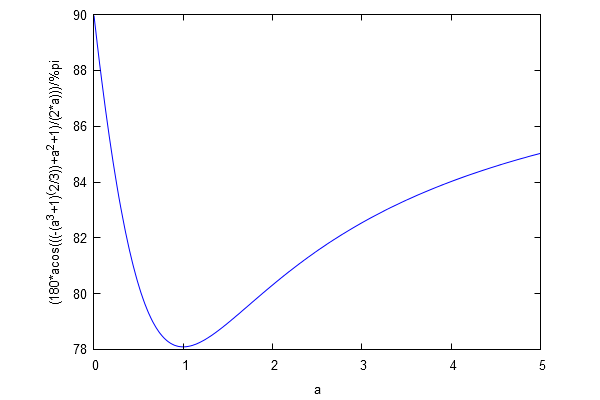
\includegraphics[width=1.1\linewidth]{FLT_angle_n_3.png}
  \caption{Angle plot for triangle $(a, 1, \sqrt{a^3 + 1^3})$}
  \label{fig:angle_n_3}
\end{subfigure}%
\begin{subfigure}{.5\textwidth}
  \centering
  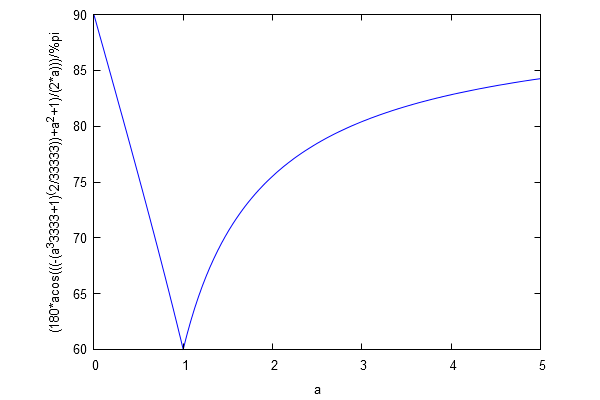
\includegraphics[width=1.1\linewidth]{FLT_angle_n_33333.png}
  \caption{Angle plot for $(a, 1, \sqrt{a^{33333} + 1^{33333}})$}
  \label{fig:angle_n_33333}
\end{subfigure}
\caption{For both plots, vertical axis is the angle between the 2 sides of triangle $a$ and $b$ with a fixed $b$ normalized to $1$}
\label{fig:FLT_angle}
\end{figure}
%

The angle $\theta$ between $a$ and $b$ is {\it not} fixed for $n \ge 3$. The angle always starts off at $90^\circ$ when $r_1 = 1$ and will quickly plummet as $r_1$ increases, Fig.~\ref{fig:angle_n_3}. It will then climb back up {\it asymptotically} to $90^\circ$. As we go higher in $n$, the initial dip and rebound will become more drastic but the overall behavior will remain the same, Fig.~\ref{fig:angle_n_33333}. So there is a clear dichotomy of the behavior of the angle for $n=1,2$ and $n \ge 3$.

As I was thinking about what this might mean I was reminded of Galois theory (you might want to check Wildberger's youtube lecture on this as an introduction, see his history of mathematics series). The reason why quintic equations have no solution is because the symmetry structure does not cascade as it does for quartic and below. Can it be that a symmetry structure plays a role here as well? If so, what kind of symmetry?

Since the triangle formed by $a$, $b$, and $c$ is a right triangle only for $n=2$ I imagine it has something to do reflection symmetry with respect to the $x$ and $y$ axes in the cartesian coordinate. Say the triangle is given by these three points $(0, 0)$, $(a, 0)$, and $(0, b)$, by doing horizontal and vertical reflections (plus translations) we can cover the entire cartesian plane, \eg a reflection w.r.t the $x$ axis generates the triangle $(0,0) (a,0) (0,-b)$ while a subsequent relection w.r.t the $y$ axis gives $(0,0) (-a,0) (0,-b)$. If we then translate this triangle using a vector $(a \hat x, b \hat y)$ - and combining it with our original triangle - we will get a rectangle $(0,0) (a,0) (a,b) (0,b)$, repeating this process indefinitely produces a covering for the entire cartesian plane.

Not so for $n \ge 3$, since the angle can never reach $90^\circ$ there is always some area that is not covered by the above symmetry operations. From this observation, the symmetry of interest is the discrete symmetry $Z_2$ (plus some translation symmetry).

\bigskip\textbf{\textit{Idea \#2}}

At this point I'm not sure what this all means, or if it is actually profitable to pursue this line of thought since I can't find anything concrete to say about it.

My next idea is whether there is a higher dimensional object that represents $a^n + b^n = c^n$ for different $n$'s. Since $n=2$ is a triangle maybe $n \ge 3$ is some 3d object (after all $a^3 + b^3$ means that we are adding two volumes to get a third one) and $n=4$ is an even higher dimensional object and so on. But again, I don't know what to make of it.

\bigskip\textbf{\textit{Idea \#3}}

I then was reminded of quantum mechanics. Before learning quantum mechanics I wouldn't even imagine of something that have discrete and continuum spectrum in one solution but there is (there are actually plenty examples in quantum mechanics). How is it related to Fermat? Because in Fermat, $a^n + b^n = c^n$ happens to just miss all of the integers $a,b,c$ for $n \ge 3$ (while taking in real values just fine). So these seems like the inverse hydrogen atom, instead of having discrete spectrum it has an inverse discrete spectrum where all integers are skipped (is there such a physical object in the universe?).

So maybe there's a differential equations that yield a solution where all integers are skipped? can we just do a Fourier transform of $a^n + b^n = c^n$? Just a wild guess :)

\bigskip\textbf{\textit{Idea \#4}}

Another strange idea I came up with was again inspired by symmetry. Say we move to the complex plane, does $a^n + b^n = c^n$ exhibit conformal symmetry? dilatation symmetry?

Why do they even relate to Fermat? It's all about angles! Back to idea \#1, the angles between the two line segments $a$ and $b$ is always fixed for $n=2$, this somewhat resembles conformal symmetry where the angle between two lines is always preserved. So maybe there's a conformal/dilatation symmetry preserved by $n=2$ which is not preserved by $n \ge 3$. Again, just a wild guess, nothing concrete :)

\bigskip\textbf{\textit{Fun Excursions}}

Since the above ideas didn't get me anywhere I was thinking about other aspects of Fermat. We know we can't find solutions with just two numbers $a$ and $b$, how many numbers do we need to get a solution? \ie $a^n + b^n  + d^n + ... = c^n$.

So I began with $n=3$, and lo and behold, I found integer solutions for $a^3 + b^3  + d^3 = c^3$. Do these solutions have a pattern behind them? Euclid to the rescue ... (maybe)

\bigskip\textbf{\textit{Running along Euclid}}

Euclid (some people said it was the Babylonians) gave us an algorithm to find the solutions of $a^2 + b^2 = c^2$, which is as follows
%
\nbea
(m^2 - n^2)^2 + (2mn)^2 & = & (m^2 + n^2)^2
\neea
%
you simply pluck in whatever integers you fancy into $m$ and $n$ and Voila! you get a Pythagorean solution (one is usually interested in co-prime solutions, \ie $a,b,c$ have no common divisor). So maybe a similar algorithm exists for $a^3 + b^3  + d^3 = c^3$?

Well, there are actually plenty of algorithms for $a^3 + b^3  + d^3 = c^3$. They are categorized by how many parameters are used and more imprtantly by what solutions they produce, it turns out that the different algorithms generate only selective solutions or families unlike the Babylonian algorithm above which generate every solution for the Pyhtagorean equation.

The algorithm above is a two parameter algorithm, there is actually a one parameter algorithm as well. But before we discuss all this let me show you my misadventures with these algorithms as I try to wildly guess what they might be like.

\bigskip\textbf{\textit {Euclidean roullette}}

What we really want to know is how those Babylonians or Euclid came up with the formula (or they might have just been really smart and saw the solution immediately, me no Euclid). At a glance it looked like just a good guess. So let say we start with a simplest of most guesses
%
\nbea
a^2 + (a+y)^2  & = & (a + z)^2
\neea
%
we see that the solution for $a$ has to be
%
\nbea
(a + z)^2 - \left \{ (a+y)^2 + a^2 \right \} & = & z^2 + 2 a z - y^2 - 2 a y - a^2 = 0 \\
\rightarrow a & = & \pm \sqrt{2}\sqrt{z^2 - yz} + z - y
\neea
%
which in turn means that
%
\nbea
z^2 - yz & = & 2 w^2
\neea
%
for some integer $w$. One obvious solution is
%
\nbea
z & = & 2w \\
y & = & w \\
a & = & 2w + 2w - w = 3w \\
\rightarrow (3w)^2 + (4w)^2 & = & (5w)^2
\neea
%
And we get the $3,4,5$ solution and its integer multiples. There are actually many other solutions for $z^2 - yz = 2 w^2$, this turns out to be a blessing in disguise, we shall see this in a little bit.

Now, what happens if we choose a different starting point?
%
\nbea
a^2 + (a \cdot y)^2  & = & (a + z)^2 \\
(a + z)^2 - \left \{ (a \cdot y)^2 + a^2 \right \} & = & z^2 + 2 a z - a^2 y^2 = 0 \\
\rightarrow a & = &\frac{z \pm \sqrt{y^2 + 1}}{y^2}
\neea
%
This time, we can only solve it if we change $y$ into a rational number $p/q$ but solving $p^2/q^2 + 1 = r^2/s^2$ is just solving the Pythagorean equation in the first place. However, the above equation also means
%
\nbea
(a y^2 - z)^2 & = & y^2 + 1 \\
a^2 y^4 - 2 a y^2 z + z^2 & = & y^2 + 1 \\
a^2 p^4 - 2 a p^2 q^2 z + z^2 & = & p^2 q^2 + q^4
\neea
%
So why all this asinine substitutions?

\bigskip\textit{\textbf{Lagniappe}}

I wanted to say ``small lagniappe'' but lagniappe itself is already small :) The above two examples actually show us how to use Euclid's algorithm to solve other equations (instead of generating a new algorithm to solve the pyhtagorean equation). The first example
%
\nbea
z^2 - yz & = & 2 w^2
\neea
% 
can be paraphrased into the Pythagorean equation, because it was a consequence of
%
\nbea
a^2 + (a+y)^2 & = & (a+z)^2 \\
(m^2-n^2)^2 + (2mn)^2 & = & (m^2+n^2)^2
\neea
%
which means that
%
\nbea
a & = & m^2-n^2 \\
a + y & = & 2mn \\
a + z & = & m^2 + n^2
\neea
%
By solving the above equations, the algorithm for the solutions of $z^2 - yz = 2 w^2$ is then
%
\nbea
z = 2 n^2,~~ y = n^2 + 2mn -m^2, ~~w = n^2 (n - m)^2
\neea
%
\ie we can choose any two integers $m$ and $n$ and the integer solutions for $z^2 - yz = 2 w^2$ are given above (note that we can also choose $a = -(m^2 - n^2)$ generating a slightly different final result).

It's the same with $a^2 p^4 - 2 a p^2 q^2 z + z^2 = p^2 q^2 + q^4$, equating terms just like before gives
%
\nbea
a = m^2-n^2, ~~ z = 2 n^2,~~ y = \frac{p}{q} \rightarrow p = 2mn, q = m^2 - n^2
\neea
%
I called the above lagniappe because it was just a small boon. The boon is that there's actually a way to solve these seemingly random equations, \eg $z^2 - yz = 2 w^2$, $a^2 p^4 - 2 a p^2 q^2 z + z^2 = p^2 q^2 + q^4$. However, those solutions we found above are not unique because Euclid's algorithm itself is not unique, as we shall see.

There's also another fun thing related to this, if we start with
%
\nbea
(a+z)^2 + (a-z)^2 & = & (a \cdot y)^2 \\
(a+z)^2 + (a-z)^2 - (a \cdot y)^2 & = & -2 z^2 + a^2 y^2 - 2 a^2 = 0
\neea
%
we can now choose which one to solve
%
\nbea
{\rm solving ~} y:~ y & = & \pm \frac{\sqrt{2}\sqrt{z^2 + a^2}}{a} \\
{\rm solving ~} z:~ z & = & \pm \frac{a\sqrt{y^2 - 2}}{\sqrt{2}} \\
{\rm solving ~} a:~ a & = & \pm \frac{\sqrt{2}z}{\sqrt{y^2 - 2}}
\neea
%
note that we are not solving $y$ followed by $z$ followed by $a$, we are only solving {\it one} of them but since we have three variables we can choose which one to solve. We then have the following constraints
%
\nbea
{\rm from~solving~}y{\rm~we~get}:~~z^2 + a^2 & = & 2w^2 \\
{\rm from~solving~}z{\rm~or~}a{\rm~we~get}:~~2 u^2 + 2 & = & y^2
\neea
%
matching terms $(a+z)^2 + (a-z)^2 = (a \cdot y)^2 \rightarrow (m^2-n^2)^2 + (2mn)^2 = (m^2 + n^2)^2$
%
\nbea
a & = & m^2-n^2 + 2mn \\
z & = & m^2-n^2 - 2mn \\
y & = & \frac{2(m^2 + n^2)}{m^2-n^2 + 2mn} \\
\rightarrow w & = & m^2 + n^2 \\
\rightarrow u & = & \frac{n^2 + 2mn - m^2}{n^2 - 2mn - m^2}
\neea
%
Note that we have inserted factor of 2 where convenient :) It is now obvious that we can play this game forever, just substitute any function you fancy into the Pythagorean equation and match terms, just be careful about factors of 2.

The moral of the story here is that the Babylonians actually gave us quite a powerful tool to solve deophantine equations (if we can massage them into the Pythagorean one), these ancient people were not just good at building towers :) But in a broader sense it means that we can map one Diophantine equation into a simpler one, which is good.

\bigskip\textbf{\textit{Euclidean bulldozer}}

We now come back to the subject of utilizing unsophisticated guesses in meting out algorithms such as Euclid's. The first attempt above $a^2 + (a+y)^2 = (a+z)^2$ wasn't fruitful and in a glance this should be the same as $(a+x)^2 + (a+y)^2 = (a+z)^2$ since we can always shift $a+x \rightarrow a$. However, it is not true. Adding an extra degree of freedom like $x$ is a big deal, how big? let's see.

We can by brute force find an algorithm for $a^2 + b^2 = c^2$ from the most generic starting point
%
\nbea
(a+z)^2 & = & (a+x)^2 + (a+y)^2 \\
(a+z)^2 - \{(a+x)^2 + (a+y)^2\} & = & z^2+2az-y^2-2ay-x^2-2ax-a^2 = 0
\neea
%
Now we have four choices, we can solve for either, $a$, $x$, $y$, or $z$, which one we solve determines our fate. Solving for $a$ gives
%
\nbea
a = z-y-x \pm \sqrt{2}\sqrt{z^2+(-y-x)z+xy}
\neea
%
which means that
%
\nbea
z^2+(-y-x)z+xy & = & 2 p^2 \\
\rightarrow x & = & \frac{z^2-yz-2p^2}{z-y} \\
\rightarrow a & = & -\frac{(y+2|p|)z-y^2-2|p|y-2p^2}{z-y}
\neea
%
and there we have it, the full algorithm is
%
\nbea
\begin{array} {l c l c l}
a + x & = & z-y-2|p| & \rightarrow & (z-y-2|p|)(z-y) \\
a + y & = & -\frac{2|p|z-2|p|y-2p^2}{z-y}  & \rightarrow & 2|p|z-2|p|y-2p^2 \\
a + z & = & \frac{z^2+(-2y-2|p|)z+y^2+2|p|y+2p^2}{z-y}  & \rightarrow & z^2+(-2y-2|p|)z+y^2+2|p|y+2p^2
\end{array}
\neea
%
we can multiply each term by $(z-y)$ if we want to and flip the minus sign. So apparently we can just go by brute force to bulldoze out an algorithm, in this case we have {\it three} final degrees of freedom.

However, we can also solve $x$ first
%
\nbea
x & = & -a \pm \sqrt{z^2+2az-y^2-2ay}
\neea
%
The next step is crucial, do we solve for $a$ or $y,z$? Let's see, solving for $a$ gives
%
\nbea
a & = & -\frac{z^2-y^2-p^2}{2z-2y}
\neea
%
which is all well and good. Had we chosen to solve for $y$ we'd have gotten
%
\nbea
y & = & -a \pm \sqrt{z^2+2az-p^2+a^2}, ~~{\rm solving~for~}a~{\rm next} \\
\rightarrow a & = & -z \pm \sqrt{q^2+p^2} ~~~{\rm OR~solving~for~}z~{\rm next}\\
\rightarrow z & = & -a \pm \sqrt{q^2+p^2}
\neea
%
Solving either $a$ or $z$ produces no headway since now we have to solve for $q^2+p^2 = r^2$ which is our original problem. Thus the order we choose to solve the degrees of freedom matters. Can we follow the same mechanical steps to arrive at algorithms for $a^3 + b^3 + c^3 = d^3$?

\bigskip\textbf{\textit{Cubic conundrum}}

Applying the same guessing strategy to $a^3 + b^3 + c^3 = d^3$ turns out to be tricky. My first attempt was $a^3 + (a+y)^3 + (a+z)^3 = (a+w)^3$ but the cube root of a square root (generated by solving $a$ in terms of $y,z,w$) was too hard to handle.

The next natural progression is of course $(a+x)^3 + (a+y)^3 + (a+z)^3 = (a+w)^3$ to allow more flexibility but just like the preceding attempt the resulting equations quickly became intractable. My next attempt was to simplify things by adding a minus sign $(a+x)^3 + (-a+y)^3 + (a+z)^3 = (a+w)^3$ such that we no longer have $a^3$, however even with this modification the equations were still too long to be discernible
%
\nbea
&& (a+w)^3 - \{(a+x)^3 + (-a+y)^3 + (a+z)^3 \} = 0\\
&& ~~~~~~~~~~~\Longrightarrow a ~~= ~ (6z+6y+6x-6w)^{-1} (-3z^2+3y^2-3x^2+3w^2 \\
&& ~~~~~~~~~~~~~~~~~~~~~~~~~~~~ \pm \sqrt{3} (-z^4+(-4y-4x+4w)z^3+(-6y^2+6x^2-6w^2)z^2+ \\
&& ~~~~~~~~~~~~~~~~~~~~~~~~~~~~ (-4y^3-4x^3+4w^3)z-y^4 + (4w-4x)y^3+(6w^2-6x^2)y^2+ \\
&& ~~~~~~~~~~~~~~~~~~~~~~~~~~~~ (4w^3-4x^3)y-x^4+4wx^3-6w^2x^2+4w^3x-w^4 )^{1/2})
\neea
%
here we have a super long square root (no more cube root since we have no $a^3$). The problem with this square root is that it contains fourth powers $z^4, y^4, x^4$. Solving for $x, y$ or $z$ inside the square root generates more problems, \ie roots containing higher powers which in turn generates more complicated equations.

My final attempt was $(a+x)^3 + (-b+y)^3 + (b+z)^3 = (a+w)^3$ however, solving $a$ or $b$ still generates ridiculously long square roots, solving for $x$ however seems to be a lot simpler
%
\nbea
x & = & (-z^3-3az^2-3a^2z-y^3-3by^2-3b^2y+w^3+3aw^2+3a^2w-b^3)^{1/3}+b
\neea
%
We are now faced with the same decision tree as discussed previously, who's next? Turns out that solving for $y,z$ or $w$ generates $p^3+q^3+r^3 = s^3$ just like the Pythagorean case above. Seems like we need to solve $b$ or $a$ first but $b$ gives a better outcome
%
\nbea
b & = & (-z^3-3az^2-3a^2z+w^3+3aw^2+3a^2w-p^3)^{1/3}+y
\neea	
%
It looks good as $y$ decouples. Next we need to solve for $a$, solving any other variables generates $p^3+q^3+r^3 = s^3$
%
\nbea
a & = & \left (3z^2-3w^2 \pm \sqrt{3}\sqrt{-z^4+4wz^3-6w^2z^2+(4w^3-4q^3-4p^3)z-w^4+(4q^3+4p^3)w} \right ) \times \\
&& (6z-6w)^{-1}
\neea	
%
That long square root is a killer, solving it for $z$ or $w$ generates a root of a cube root of a root of a root, {\it four} nested roots! {\it Q.E.D} ({\it Q}.uickly {\it E}.nded {\it D}.reams)

In short, a brute force guessing game might be theoretically possible but not recommended :) in other words, it works well for certain obvious cases and thus it only has a very limited merit.

\bigskip\textbf{\textit{Euclidean apery}}

We now go back to guessing our own version of an algorithm for the Pythagorean equation (without a bulldozer). In our case, the goal here is to solve $a$ in terms of two completely free parameters $z$ and $y$. Let's try one with a quite generic structure
%
\nbea
(a - z)^2 + (a\cdot y)^2  & = & (a + z)^2 \\
(a + z)^2 - \left \{ (a \cdot y)^2 + (a - z)^2 \right \} & = & 4 a z - a^2 y^2 = 0 \\
\rightarrow a & = & \frac{4 z}{y^2}
\neea
%
Yay! It works! (the other solution is $a=0$). The full solution is then
%
\nbea
\left ( \frac{4 z}{y^2} - z\right )^2 + \left ( \frac{4 z y}{y^2} \right )^2 & = & \left ( \frac{4 z}{y^2} + z\right )^2 \\
\Rightarrow \left ( 4 z - z y^2\right )^2 + \left ( 4 z y \right )^2 & = & \left ( 4 z + z y^2\right )^2
\neea
%
Although this is different from Euclid's, given any integer $z$ and $y$ we can generate a solution. Looks like these algorithms are not unique (as advertised) although I'm not sure (or too lazy to prove) that this version covers all solutions of the Pythagorean equation.

A more straighforward guess will be
%
\nbea
(a + z)^2 - (a - z)^2 & = & 4az
\neea
%
we can simply promote $a \to a^2, z \to z^2$ to get
%
\nbea
(a^2 + z^2)^2 - (a^2 - z^2)^2 & = & 4a^2z^2 = (2az)^2
\neea
%
which is Euclid's (or the Babylonians').

So the trick in this guessing game is that you guess a term on the LHS and another on the RHS. You then want the difference between those two sides {\it not} to be a sum of terms, because then you're just going back to square one by needing to solve some equation in the form of $x_1^{n_1} + x_2^{n_2} = a^m$. For example, if you're naively try to solve fermat's cubic last theorem the same way
%
\nbea
(a-z)^3 + X^3 & = & (a+z)^3 \\
\rightarrow X^3 & = & 2z^3 + 6a^2 z
\neea
%
You just get another deophantine equation to solve, back to square one.

One thing to note here is that we at first assume that all terms in our guess has the same power, \eg $a, z$ both have the power of one, we can for example promote things to $a^n, z^m$ but our goal for now is to see how far these simple guesses take us.

\bigskip\textbf{\textit{Jabs in the dark}}

We now begin our journey in guessing the form of algorithm for $a^3 + b^3 + c^3 = d^3$.
\begin{enumerate}
\item I first tried the following solution (which looks simplest of all)
%
\nbea
a^3 + b^3 + K^3  & = & (a + b)^3
\neea
%
with some unknown integer $K$ (in Euclid's case $K$ is just $2mn$). Let's see if we get lucky. Now $K^3$ is obviously $3 a b (b + a)$. Sadly, the only solution is $a = 1$, $b = 8$, $K=6$ and their integer multiples. 

We can try setting $a = 3^2 c^3$. First, why this choice? The goal here is to make $3a$ into $3a=P^3$ for some integer $P$. So the first thing to do is to complete the factor 3 into $3^3$ by multiplying it by $3^2$. What we need next is $b (b + a) = N^3$ which we will solve later. With this choice $3 a b (b + a) = 3^3 c^3 N^3 = K^3 \rightarrow K = 3 c N$ we would have found our algorithm. However, even with this scheme, the only solutions are integer multiples of $a = 1$, $b = 8$, $K=6$.

\item From the list of solutions for $a^3 + b^3 + c^3 = d^3$ I saw a familiar face $3, 4, 5, 6$ (by the way, the tuplet $3,4,5,6$ also represent the sides of a right triangle $3,4,5$ with an area of $6$). Prompting me to guess a solution of the form
%
\nbea
a^3 + (a+1)^3 + (a+2)^3  & = & (a + 3)^3 \\
(a + 3)^3 - (a^3 + (a+1)^3 + (a+2)^3) & = & 2 (3 - a) (a^2 + 3a + 3) = 0
\neea
%
The last equation shows that this scheme will only work for $a = 3$, no other solution is sequential.

\item What if we mix products and additions of terms? Like this one
%
\nbea
a^3 + (a \cdot x)^3 + (a \cdot y)^3 & = & (a + z)^3 \\
(a + z)^3 - \left \{ a^3 + (a \cdot x)^3 + (a \cdot y)^3 \right \} & = & z^3 + 3 a z^2 + 3 a^2 z - a^3 y^3 - a^3 x^3
\neea
%
Now this doesn't look promising to some since we can always factor out $a$ to get $y^3 + x^3 + 1 = w^3$, however, from our previous discussion about shifting $a + z \to a$, we know that adding a degree of freedom actually makes a difference. So let give this a shot. The solution is
%
\nbea
a & = & \frac{z \left \{ (y^3 + x^3 + 1)^{2/3} + (y^3 + x^3 + 1)^{1/3} +1 \right \} }{(y^3 + x^3) }
\neea
%
while the other two solutions give imaginary $a$. Which is rather disappointing since we now need to solve
%
\nbea
y^3 + x^3 + 1 & = & w^3
\neea
%
so this time adding a degree of freedom doesn't help. If we insist in substituting the solution for $a$ the factor $z$ cancels from both LHS and RHS and the only free variables in $a^3 + (a \cdot x)^3 + (a \cdot y)^3 = (a + z)^3$ are just $x$ and $y$ which is the same free variables we have in $y^3 + x^3 + 1 = w^3$.

At this point I would like to list solutions of $y^3 + x^3 + 1 = w^3$, see Table~\ref{Tab:1} (sorted in ascending $x$). One can immediately see that $y=138$ gives us {\it two} different sets of solutions ($426$ also gives two solutions but once as $x$ and another as $y$). Also, from their prime factors we can see that the solutions are all co-prime to one another.

Another thing to note is that the difference $y-x$ and $w-y$ are all different for different solutions, showing that an algorithm, \ie $a^3 + (a+m)^3 + (a+n)^3 = (a + p)^3$ where $m,n,p$ are {\it fixed} will not work as each fixed difference $m,n,p$ will only give a single solution. 

In addition, this also means that it is a near miss for Fermat, $a^3 + b^3 = c^3$ has no solutions but $1 + a^3 + b^3 = c^3$ does :)

One last comment on this topic, we can arrange things differently $y^3 + x^3 + 1 = w^3 \rightarrow y^3 + x^3 = w^3 - 1$
%
\nbea
y^3 + x^3 & = & w^3 - 1 \\
& = & (w-1)(w^2+w+1) \\
& = & (w-1)((w-1)^2+3w) \\
& = & (w-1)^3 + 3w(w-1)
\neea
%
We can now add degrees of freedom as usual $y = b+z, ~ x = b-z$
%
\nbea
(b+z)^3 + (b-z)^3 & = & (w-1)^3 + 3w(w-1) \\
6bz^2+2b^3 & = & (w-1)^3 + 3w(w-1)
\neea
%
This looks promising as we have the same number of terms in both LHS and RHS. We know that $2b^3$ can't be $u^3$ for some integer $u$ due to the factor of 2, the easiest algorithm for $y^3 + x^3 + 1 = w^3$ is to set $2b^3 = 3w(w-1), ~ 6bz^2 = (w-1)^3$. However, from the $1,6,8,9$ solution it is clear that we cannot make such identification.

We can try adding more variables, \eg $1=(b-z-a), y=(b+z)$, but this only complicates things with no clear benefit. In other words, only the combination, \eg $6bz^2+2b^3$, constitutes $x_1^3 + x_2^3$, we cannot cast any one term $6bz^2$ or $2b^3$ as a pure power of 3, $6bz^2 = p^3$ or $2b^3 = q^3$.

\item Another potential solution is
%
\nbea
(a-b)^3 + (b-c)^3 + (c-a)^3 & = & 3 (a-b)(b-c)(c-a)
\neea
%
The nice thing is that the RHS is not a sum of terms, so we have a chance if we set
%
\nbea
(a-b)(b-c)(c-a) & = & 3^2 w^3
\neea
%
To simplfy things let's denote $p = (a-b)$, $q = (b-c)$, $r = (c-a)$
%
\nbea
p \cdot q \cdot r & = & 3^2 w^3\\
p + q+ r & = & 0
\neea
%
We can solve the above equations by substituting $p = 3^2 w^3/qr$ into $p + q+ r = 0$
%
\nbea
0 & = & 3^2 w^3 + q^2 r + q r^2 \\
\rightarrow r & = & \frac{-q^2 \pm \sqrt{q^4 - 36 \cdot q \cdot w^3}}{2 q}
\neea
%
To ensure that $r$ is an integer, $q^4 - 36 q w^3 = v^2$ for some integer $v$. The interesting thing is that there are only two solutions I can find for this to happen
%
\nbea
q \rightarrow q,~w\rightarrow -2q & ~:~ & q^4 - 36 q (-2q)^3 = 289 q^4 = (17 q^2)^2 \\
q \rightarrow 4q,~w\rightarrow -q & ~:~ & (4q)^4 - 36 (4q) (-q)^3 = 400 q^4 = (20 q^2)^2 
\neea
%
Regrettably this provision will only give one solution
%
\nbea
(8q)^3 + (q)^3 + (-9q)^3 & = & (-6q)^3
\neea
%
which is just a multiple of the $1,6,8,9$ solution.

We can do some minor rearrangement
%
\nbea
p^3 + q^3 + 3 p q (p+q) & = & (p+q)^3 \\
\to (3p^3)^3 + (3q^3)^3 + (3 p q z)^3 & = & (z^3)^3 ~~~z^3 = 3p^3 + 3q^3~~~{\rm OR}\\
\to (3^2p^3)^3 + (q^3)^3 + (3 p q z)^3 & = & (z^3)^3~~~z^3 = 3^2p^3 + q^3~~~{\rm OR}\\
\to (3p^3)^3 + (q^3)^3 + (3 p q z)^3 & = & (z^3)^3~~~3z^3 = 3p^3 + q^3~~~{\rm OR}\\
\to p^3 + q^3 + z^3 & = & (p+q)^3~~~z^3 = 3 p q(p+q)
\neea
%
we can either lump the factor of $3^2$ into one of the variables or spread it onto any two of them or  assume the whole thing $3 p q(p+q)$ is a power of three $z^3$. I got some interesting result from this exercise, \eg the {\it largest} solution I found from this simple guessing game is
%
\nbea
59707533^3 + 2268747144^3 + 981751158^3 & = & 2328454677^3
\neea
%
this one was from $p \to 3 p^3, ~ (p+q) \to 3 u^3$.

\item Another promising solution is 
%
\nbea
(m-n)^3 + n^3 + A^3 & = & (m+n)^3 \\
\rightarrow A^3 & = & n^3 + 6 m^2 n
\neea
%
We can solve for $m$ or $n$ or $A$, but $m$ seems to yield the easiest solution, which is
%
\nbea
m & = & \pm \sqrt{\frac{\frac{A^3}{n} - n^2}{6}}
\neea
%
Sadly, this only gives 2 integer solutions, they are
%
\nbea
m-n = 17 ~~~ n = 4 ~~~ A = 22 ~~~ m+n = 25 \\
m-n = -2 ~~~ n = 9 ~~~ A = 15 ~~~ m+n = 16
\neea
%
I was hoping that these conditions, \eg $m = \pm \sqrt{\frac{\frac{A^3}{n} - n^2}{6}}$ or $r = \frac{-q^2 \pm \sqrt{q^4 - 36 \cdot q \cdot w^3}}{2 q}$ would yield a class of integer solutions instead of just one (or two).

So it looks like there's really no solution for $a^3 + b^3 + c^3 = d^3$ if we start we just simple guesses. 



\end{enumerate}


















%
\begin{table}[]
\centering
\caption{$(x)$ means prime factors of $x$}
\label{Tab:1}
\begin{tabular}{|c|c|c|c|c|c|}
\hline
$x$ & $y$ & $w$ & $(x)$ & $(y)$ & $(w)$ \\ \hline 
6 & 8 & 9 & $(2, 3)$ & $(2^3)$ & $(3^2)$ \\
71 & 138 & 144  & $(71)$ & $(2,3,23)$ & $(2^4, 3^2)$ \\
135 & 138 & 172  & $(3^3, 5)$ & $(2,3,23)$ & $(2^2, 43)$ \\
236 & 1207 & 1210  & $(2^2,59)$ & $(17,71)$ & $(2,5,11^2)$ \\
242 & 720 & 729  & $(2, 11^2)$ & $(2^4, 3^2, 5)$ & $(3^6)$ \\
372 & 426 & 505  & $(2^2,3,31)$ & $(2,3,71)$ & $(5,101)$ \\
426 & 486 & 577  & $(2,3,71)$ & $(2,3^5)$ & $(577)$ \\
566 & 823 & 904  & $(2,283)$ & $(823)$ & $(2^3,113)$ \\
575 & 2292 & 2304  & $(5^2,23)$ & $(2^2,3,191)$ & $(2^8,3^2)$ \\
791 & 812 & 1010  & $(7,113)$ & $(2^2,7,29)$ & $(2,5,101)$ \\
1124 & 5610 & 5625  & $(2^2,281)$ & $(2,3,5,11,17)$ & $(3^2,5^4)$ \\
1938 & 2820 & 3097  & $(2,3,17,19)$ & $(2^2,3,5,47)$ & $(19,163)$ \\
1943 & 6702 & 6756  & $(29,67)$ & $(2,3,1117)$ & $(2^2,3,563)$ \\
2196 & 5984 & 6081  & $(2^2,3^2,61)$ & $(2^5,11,17)$ & $(3,2027)$ \\
2676 & 3230 & 3753  & $(2^2,3,223)$ & $(2,5,17,19)$ & $(3^3,139)$ \\ \hline
\end{tabular}
\end{table}
%

\bigskip\textbf{\textit{Expanding the horizon}}

Finding a generic algorithm for $a^3 + b^3 + c^3 = d^3$ just by guessing seems to be quite problematic as we have seen above. So what if we add another number? Say
%
\nbea
a^3 + b^3 + c^3 + d^3 & = & e^3
\neea
%
Going back to our symmetrical solution
%
\nbea
(a-z)^3 + \Delta & = & (a+z)^3 \\
\rightarrow (a+z)^3 - (a-z)^3 = \Delta & = & 2z^3 + 6a^2 \\
\Delta & = & z^3 + z^3 + 6a^2 z
\neea
%
so as long as $a^2 = 6^2 w^6$ and $z = v^3$ the above solution works since every term is a power of 3. The full solution is then
%
\nbea
(a^3 - 6^2 b^6)^3 + (6^2 b^6)^3 + (6^2 b^6)^3 + (a^2 \cdot 6 b^2)^3  & = & (a^3 + 6^2 b^6)^3
\neea
%
But I don't like this solution since it contains a constant factor $2$. There's yet another solution, if we began with
%
\nbea
(-a+b+c)^3 + (a-b+c)^3 + (a+b-c)^3 + X & = & (a+b+c)^3\\
\rightarrow X & = & 24 a b c
\neea
%
The above approach works as there is a so called ``symmetry'' where all complicated terms cancel for LHS and RHS. This was done by alternating the minus sign in each term to make sure there is only one $a^3, b^3, c^3$ on the LHS as there is on the RHS. Now, since $X$ is just a product of terms the most obvious choice would be $a \rightarrow a^3, b \rightarrow b^3, c \rightarrow 3^2 c^3$. The full solution is then
%
\nbea
(-a^3 + b^3 + 3^2 c^3)^3 + (a^3 - b^3 + 3^2 c^3)^3 + (a^3 + b^3 - 3^2 c^3)^3 + (2 \cdot 3 \cdot a b c)^3  & = & (a^3 + b^3 + 3^2 c^3)^3
\neea
%
There are other choices as well like $a \rightarrow a^3, b \rightarrow 3 b^3, c \rightarrow 3 c^3$. A more generic solution would be $a \rightarrow a^{3 \cdot m_1}, b \rightarrow 3 \cdot K_1^{3 \cdot n_1} b^{3 \cdot m_2}, c \rightarrow 3 \cdot K_2^{3 \cdot n_2} c^{3 \cdot m_2}$ but this also allows for something else, namely $a^3 + b^3 + c^3 + d^N = e^3$ by setting $a \rightarrow 2^{N-3} 3^{N-1} a^{N},~2^3 \cdot 3~ abc \rightarrow 2^3 \cdot 3~ (2^{N-3} 3^{N-1} a^{N}) b^{N} c^{N}  = (2 \cdot 3~abc)^N$, \ie
%
\nbea
(2^{N-3} 3^{N-1} a^{N} + b^N + c^N)^3 & = & (-2^{N-3} 3^{N-1} a^{N} + b^N + c^N)^3 + (2^{N-3} 3^{N-1} a^{N} - b^N + c^N)^3 + \\
&& (2^{N-3} 3^{N-1} a^{N} + b^N - c^N)^3 + (2 \cdot 3 a b c)^N
\neea
%

The most general solution would be to distribute the prime factors of $P^3 (\equiv 24 abc)$ into $a$, $b$, and $c$,
%
\nbea
P = \prod_{i=1}^{L} p_i^{n_i} ~~~\longrightarrow~~~ P^3 = \prod_{i=1}^{L} p_i^{3 n_i}
\neea
%
where each $p_i$ is a prime number, $n_i$ the multiplicity of $p_i$ and $L$ the number of different prime factors of $P$ and the probability is infinite :)

One way we can use our newly found expanded horizon is to set one of the terms, $(-a+b+c)$ or $(a-b+c)$ or $(a+b-c)$, to zero, since we can't set the product term $24abc$ to zero without resulting in a trivial pursuit :)

By setting one of the terms above to zero we would get our prime objective $a^3 + b^3 + c^3 = e^3 $ from $a^3 + b^3 + c^3 + \cancel{d^3} = e^3$. However, this exercise proves futile as the only solution generated is the infamous $1,6,8,9$, \ie $a = 1, b = 2, c = 1 \rightarrow -9a^3 + b^3 + c^3 = 0$.

There is a  possible (and potential) use of the above algorithm. Say we start with $(a+z)^3$ and $(a+y)^3$ on the LHS and RHS respectively, what we want is
%
\nbea
(a+z)^3 & = & (a+y)^3 + C_1^3 + C_2^3 \\
(a+z)^3 - (a+y)^3 & = & 3 a^2 z + 3 a z^2 + z^3 - (3 a^2 y + 3 a y^2 + y^3) \\
& = & 3 a^2 z + 3 a z^2 - y^3 - (3 a^2 y + 3 a y^2 - z^3) \\
& = & (a+z)^3 - a^3 - z^3 - y^3 - ((a+y)^3 - a^3 - y^3 - z^3) \\
& = & C_1^3 - C_2^3 \\
\rightarrow C_1^3 & = & (a+z)^3 - a^3 - z^3 - y^3 \\
\rightarrow C_2^3 & = & (a+y)^3 - a^3 - y^3 - z^3
\neea
%
in the second line we need to swap $y \leftrightarrow z$ otherwise we'll get
%
\nbea
3 a^2 z + 3 a z^2 + z^3 & = & (a+z)^3 - a^3 \\
\tilde C ^3 & = & (a+z)^3 - a^3
\neea
%
which is Fermat and we don't have a solution for it. However, we now have $a^3 + b^3 + c^3 + d^3 = e^3$ for both $C_1$ and $C_2$, the bad news is that we might not be able to use the algorithm found above to solve them. The main problem is that $C_2$ has the same terms as $C_1$ on the RHS. Another problem is, even if we only consider $C_1$, matching terms to our algorithm above
%
\nbea
(a+z) & = & -p^3 + q^3 + 3^2 r^3 \\
a & = & -p^3 + q^3 - 3^2 r^3 \\
z & = & -p^3 - q^3 + 3^2 r^3 \\
y & = & - 2 \cdot 3 ~ pqr
\neea
%
the solution will be
%
\nbea
r & = & \left ( \frac{q^3 + p^3}{9} \right )^{1/3} \\
a & = & 2 q^3 \\
y & = & 2~pq~3^{1/3} (q^3 + p^3)^{1/3} \\
z & = & -2(q^3 + p^3)
\neea
%
while $p$ and $q$ remain free parameters. The above requires that 
%
\nbea
q^3 + p^3 & = & \frac{w^3}{3}
\neea
%.
and the only solution is $q = 1,~p=2, ~w=3$ (this is just the 1,6,8,9 solution with $z=0$). We could have chosen our other algorithm, \ie $a+z = -p^3 + 3 q^3 + 3 r^3$ but this choice leaves us no way out. But why did we choose $(a+z) = -p^3 + q^3 + 3^2 r^3$ in the first place? because other choices generate complex solutions :)

\bigskip\textbf{\textit{Observation intermission}}

We now take a break from guessing and start staring at the numerical solutions of $a^3 + b^3 + c^3 = d^3$ we found and take stock of what we've found so far.

First, the solutions are not unique, we have pairs of numbers that appear in more than one solution, see Table.~\ref{Tab:2}.
%
\begin{table}[]
\centering
\caption{Some sample of twins for $x^3 + y^3 + z^3 = w^3$, including one of the biggest one I found (see bottom row)}
\label{Tab:2}
\begin{tabular}{||c c c c||}
\hline
$x$ & $y$ & $z$ & $w$ \\ \hline 
3 & 36 & {\bf 37} & {\bf 46} \\
27 & 30 & {\bf 37} & {\bf 46} \\ \hline
76 & 165 & {\bf 192} & {\bf 229} \\
102 & 157 & {\bf 192} & {\bf 229} \\ \hline
{\bf 9} & 58 & 255 & {\bf 229} \\
{\bf 9} & 183 & 220 & {\bf 229} \\ \hline
58 & {\bf 201} & 255 & {\bf 292} \\
183 & {\bf 201} & 220 & {\bf 292} \\ \hline
24 & 159 & {\bf 382} & {\bf 391} \\
87 & 150 & {\bf 382} & {\bf 391} \\ \hline
~2678 & 10533 & {\bf 43420} & {\bf 43629} \\
~~5157~~& ~~10166~~ & ~~{\bf 43420}~~ & ~~{\bf 43629}~~ \\ \hline
\end{tabular}
\end{table}
%
There are in total 1290 such twins from a total of 39607 solutions (around $3\%$, solutions are generated ascendingly by $x$, the smallest number in each solution). However, this percentage depends on how we search the solution space. Twins are more likely to pop up when $x, y, z$ are relatively close, see comments in ``Intuition rumination" section.

Moreover, there are intriguing solutions like this one, where the difference between the two largerst terms is just one!
%
\nbea
462^3 + 1981^3 + 51227^3 & = & 51228^3
\neea
%

\underline{\textit{\textbf{An interesting question will be:}}} the distribution of these twins, are they spread evenly? does their precentage keep fluctuating or does it stabilize at some point or does it increase without bound? For example see Fig.~\ref{fig:twins-dist}
%
\begin{figure}
\centering
  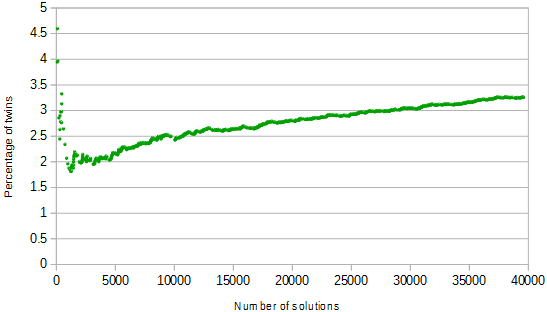
\includegraphics[width=.7\linewidth]{FLT_twins_dist.png}
  \caption{Plot of the distribution of twins among solutions of $a^3 + b^3 + c^3 = d^3$. Each green dot indicates where each twin was born among the solutions. First data point is excluded as first twins occur as solutions \#3 giving a distortedly high 33.3\% value.}
\label{fig:twins-dist}
\end{figure}
%

Second, guessing for an algorithm is not the best strategy here because there are four terms in total. It is hard to cancel terms between LHS and RHS that will result only in a product of terms as we can see from my attempts above, \eg
%
\nbea
(a+z)^3 - (a-z)^3 & = & 2 z^3 + 6 a^2 z
\neea
%
the factor of 2 in front of $z^3$ spoils everything because we need $2 z^3 = w^3$ for some integer $w$. What if we add more variables? say $(x + y +z)^3$, the problem is that there are three cubes on the RHS $x^3, y^3, z^3$ but we only have 3 terms on the LHS, this means that
%
\nbea
(x+\Delta_1)^3 + (y+\Delta_2)^3 + (z+\Delta_3)^3 & = & (x + y +z)^3
\neea
%
We can cancel $x^3, y^3,z^3$ on both sides but we now have $\Delta_1^3, \Delta_2^3, \Delta_3^3$ on the LHS (plus cross terms on both sides) that we cannot cancel.

Contrast this situation to $a^3 + b^3 + c^3 + d^3 = e^3$. If we start with $(x+y+z)^3$ on the RHS, we can cycle a minus sign on the LHS $(-x+y+z)^3$, $(x-y+z)^3$, $(x+y-z)^3$ and we will have exactly one $x^3$, $y^3$, $z^3$ on both sides with an extra term $d^3$ to absorb the rest of the cross terms. No such luck with just four terms $a^3 + b^3 + c^3 = d^3$, even if we start with two terms $(x+y)^3$ on the RHS the best I could get was
%
\nbea
(x+a)^3 + (y-a)^3 + 3 (x+a)(y-a)(x+y) & = & (x+y)^3
\neea
%
which was attempt \#4 with some minor rearrangement.

Speaking of attempt \#4 and \#5, we see something peculiar. Our usual observation says that we have  one less constraint than the number of degrees of freedom and so we should have a multitude of solutions instead of just one. Let's start with \#4, its constaints are
%
\nbea
p^3 + q^3 + r^3 & = & 3^3 w^3\\
p \cdot q \cdot r & = & 3^2 w^3\\
p + q+ r & = & 0
\neea
%
so we have 4 degrees of freedom $p,q,r,w$ with three constraints. For \#5, its {\it two} constraints are
%
\nbea
(m-n)^3 + n^3 + A^3 & = & (m+n)^3 \\
n^3 + 6 m^2 n & = & A^3
\neea
%
Again one extra free term, two constraints with {\it three} degrees of freedom $m,n,A$. The odd thing here is that the above two examples yield only one solution each, despite the extra {\it free} degree of freedom.

How can this be? This is because we are so used to thinking about real numbers. When solving a system of equations, the equations are the only constraints there are. Not so with integers/natural numbers. By requiring that the solutions are integers we are implicitly imposing another constraint, albeit a non traditional one. Going back to Fermat, $a^3 + b^3 = c^3$, we have only one constraint and three degrees of freedom and yet it has no solutions! It's because all the solutions are real numbers.

Let's see this in more detail through a concrete example

\bigskip\textbf{\textit{Attempt \#6 must die!}}

This one was exhilirating because at  a glance it gives you a lot of hope until you see it more closely. The starting point is
%
\nbea
a^3 + (y^{1/3})^3 + (a-z)^3 & = & (a + 8z)^3 \\
(a + 8z)^3 - \{a^3 + (y^{1/3})^3 + (a-z)^3\} & = & 513 z^3+189 a z^2+27 a^2 z-y-a^3 = 0
\neea
%
The funny term $(y^{1/3})^3$ is due to hindsight :) and even though in itself it is a constraint, it's irrelevant to the point I'm trying to make here. On the onset it seems like we have three degrees of freedom with only one constraint. Implying
%
\nbea
a & = & \left(\frac{\sqrt{1539648z^6-7344yz^3+y^2}}{2}-\frac{y-3672z^3}{2} \right)^{1/3} \\
&& +144z^2 \left ( \frac{\sqrt{1539648z^6-7344yz^3+y^2}}{2}-\frac{y-3672z^3}{2} \right)^{-1/3}+9z
\neea
%
To have any chance at all the inner square root has to produce an integer
%
\nbea
1539648z^6-7344yz^3+y^2 & = & u^2
\neea
%
but this is an additional constraint. One might object that it also introduces a new degree of freedom $u$. However, solving the above equation
%
\nbea
y=3672z^3 \pm \sqrt{11943936z^6+u^2}
\neea
%
This in turn means we acquire another constraint $\sqrt{11943936z^6+u^2}$ (which comes with another degree of freedom). This is a zero sum game, we are not gaining anything. We can continue with this forever!

Say we don't want to play this game, we can set
%
\nbea
1539648z^6-7344yz^3+y^2 & = & 0 \\
\rightarrow y & = & 216 z^3
\neea
%
which is good news because $216 = 6^3$ (another solution is $y = 7128 z^3$). However, by this time we have utilized two constraints, the original equation and $1539648z^6-7344yz^3+y^2 = 0$. This is no good. To see why, let's continue. 

We have one more constraint to solve, $((y-3672z^3)/2)^{1/3}$ has to be an integer, the solution is $z = -w/12$ for some integer $w$. This looks promising, we have a degree of freedom, but if you substitute this solution, $z = -w/12, ~ y = 216 z^3 = -w^3/8, ~ a = -11w/4$, \ie all terms in $a^3 + (y^{1/3})^3 + (a-z)^3 = (a + 8z)^3$ are just multiples of $w$
%
\nbea
\left ( \frac{-11 w}{4} \right )^3 + \left ( \frac{- w}{2} \right )^3 + \left ( \frac{-8 w}{3} \right )^3 & = & \left ( \frac{-41 w}{12} \right )^3 \\
\rightarrow 33^3 + 6^3 + 32^3 & = & 41^3
\neea
%
Sadly we only get one final solution $6,32,33,41$ because we have three degrees of freedom to begin with but utilize three constraints to get a solution, $a^3 + (y^{1/3})^3 + (a-z)^3 = (a + 8z)^3, ~\sqrt{11943936z^6+u^2}, ~((y-3672z^3)/2)^{1/3}$. Thus the requirement that the solutions are integers is itself a powerful constraint!

Another thing to note about the example above is that since the solution for a cubic polynomial is a cube root of a square root, $( ... + \sqrt{...})^{1/3}$, we immediately incur two constraints, one for each root.

One quick side note, I initially wanted to treat the numbers in $a^3 + b^3 + c^3 = d^3$ as vectors much like in the case of $a^2 + b^2 = c^2 \rightarrow \vec a + \vec b = \vec c$ with a right angle between $\vec a$ and $\vec b$. What would become of $\vec a + \vec b + \vec c = \vec d$? maybe there's some sort of of new cosine rule? The problem is we now deal with a generic ``parallelogram'' and for such a four-sided object the angle between any two sides is not fixed as we can always squeeze the object and the length of all sides will still stay the same. This is instartk contrast to a triangle where changing the angle between any two sides would change the length of the other side.

\bigskip\textbf{\textit{Observation intermission part deux}}

The way I initially generated the solutions was through tripply nested loops $z_1 = 1 \to 1000, z_2 = 1 \to 1000, z_3 = 1 \to 1000$ where at each iteration I checked whether $z_1^3 + z_2^3 + z_3^3$ is equal to some $w^3$.

It was a symmetrical search among $z_1, z_2,$ and $z_3$. It was very inefficient since it went rhrough things multiple times, \eg 1,6,8,9 was rediscovered multiple times through 6,1,8,9 and 8,1,6,9.

I then modified it to remove any redundancy and also made it asymmetrical $z_1 = 1 \to 5200, z_2 = z_1 \to z_1 + 10000, z_3 = z_2 \to z_2 + 50000$ because I realized that $z_1,z_2,z_3$ are sometimes quite far apart.

There were in total 39607 solutions generated. They exhibit some interesting facts. First, the difference between the smallest and largest number can be quite large. Second, there is some sort of clustering going on, \eg $z_1$ and $z_2$ are close together and $z_3$ and $w$ are also close together but the gap between $z_1,z_2$ and $z_3,w$ is quite big. Third, there's no two numbers are the same, \ie $2 z^3 + z_3^3 = w^3$ has no solution.

Finally, there are always an even number of odd numbers among $z_1,z_2,z_3,w$ which means that the sum total of all four is always even. This is actually constructive because this means that we can do this
%
\nbea
(a-z)^3 + (b+y)^3 + (b-y)^3 & = & (a+z)^3
\neea
%
we can do this because $(a+z) + (a-z) = 2a,~(b+y) + (b-y) = 2b$ and since there is always an even number of odd numbers among $z_1,z_2,z_3,w$, this is always true. Continuing in this train of thought, the parameters $a,z,b,y$ are not free, they have to satisfy
%
\nbea
(a+z)^3 - \{(a-z)^3 + (b+y)^3 + (b-y)^3\} & = & 0 \\
z^3 + 3a^2z - 3by^2 - b^3 & = & 0 \\
\to z^3 + 3a^2z = b^3 + 3y^2b
\neea
%
Some words about convention. I sorted each solution set $z_1,z_2,z_3,w$ in ascending order, \ie $z_1 < z_2 < z_3 < w$. I then paired them up according their even/odd-ness in ascending order as well. I first search if $z_1$ and $z_2$ is of the same evenness, if so $z_1 + z_2 = 2b, z_2 - z_1 = 2y$. We cannot assign $z_1,z_2$ to $a,z$ because $z_1,z_2$ are the smallest numbers of the lot, $a,z$ are derived from $z_3,w$. If $z_1$ and $z_2$ is {\it not} of the same evenness, I tried $z_1$ and $z_3$, and if they're still not of the same evenness I'd try $z_1,w$ and derive $a,z,b,y$ accordingly. 

The result was quite surprising, $b \ge z, ~ b > y,~ b+y \le a+z$, always! Also $b-z$ is always a multiple of 3, \ie $b-z = 3k$ for some integer $k$.

This also sheds some light of the twin solutions. Let's take for example the first row in Table.~\ref{Tab:2}, the first twin is
%
\nbea
3^3 + 36^3 + 37^3 & = & 46^3 \\
\to (b - y = 3)^3 + (a - z = 36)^3 + (b + y = 37)^3 & = & (a + z = 46)^3
\neea
%
with $a=41, z=5, b=20, y=17$, while the second twin is given by 
%
\nbea
27^3 + 30^3 + 37^3 & = & 46^3 \\
\to (b - y = 27)^3 + (a - z = 30)^3 + (b + y = 37)^3 & = & (a + z = 46)^3
\neea
%
with $a=38, z=8, b=32, y=5$.

\bigskip\textbf{\textit{Natural selection}}

Despite the limitation of simply guessing the algorithm for $a^3 + b^3 + c^3 = d^3$, other equations can benefit from it naturally, \eg $a^4 + b^3 + c^3 = d^4$
%
\nbea
(y+z)^4 - (y-z)^4 & = & 8 y^3 z + 8 y z^3 \\
\rightarrow (y^3-z^3)^4 + (2 y^3 z)^3 + (2 y z^3)^3 & = & (y^3+z^3)^4
\neea
%
and less natural for the $5^{\rm th}$ power
%
\nbea
(y+z)^5 - (y-z)^5 & = & 2 z^5 + 20 y^2 z^3 + 10 y^4 z
\neea
%
the factor of 2 (just like that of the $3^{\rm rd}$ power) killed it. But, we can always do some substitutionary atonement $y \rightarrow 20 y^3, z \rightarrow 2 z^3$ and massage it into
%
\nbea
(20 y^3 + 2 z^3)^5 - (20 y^3 - 2 z^3)^5 & = & (2 z^2 \cdot 2 z^3)^3 + (20 y^2 \cdot 2 z^3)^3 + (20 y^3)^4(10 \cdot 2 z^3)
\neea
%
\ie an algorithm for $a^3 + b^3 + c^4 d + e^5 = f^5$, except that this time we have a product of terms $c^4 d$ that the preceding ones didn't. Things get hairy when we go to power of 7
%
\nbea
(y+z)^7 - (y-z)^7 & = & 2 z^7 + 42 y^2 z^5 + 70 y^4 z^3 + 14 y^6 z
\neea
%
Going with three terms doesn't get much better but it is now salvageable
%
\nbea
&& (x+y+z)^7 - (-x+y+z)^7 - (x-y+z)^7 - (x+y-z)^7 \\
&& ~~~~~~~~~~~= 56 xyz (3 (x^2+y^2+z^2)^2 + 4(x^2 y^2+x^2 z^2+y^2 z^2)) \\
&& ~~~~~~~~~~~= 2 \cdot 7 \cdot 3 xyz \cdot 2^2 (x^2+y^2+z^2)^2 + 2^3 x^3y^3z \cdot 7\cdot 4 + 2^3 x^3yz^3 \cdot 7\cdot 4 + 2^3 xy^3z^3 \cdot 7\cdot 4 \\
&& ~~~~~~~~~~~= (42 xyz) (2 p^2)^2 + (2 xy)^3 (28 z)  + (2 x z)^3 (28 y) + (2 y z)^3 (28 x)
\neea
%
where $p^2 = x^2+y^2+z^2$ whose algoritm will be discussed later. You really need to be creative to appease higher powers :)

Along the same line, $a^3 + b^3 + c^3 = d^3$ can be post processed
%
\nbea
(a+z)^3 - (a-z)^3 & = & 2 z^3 + 6 a^2 z
\neea
%
substituting $z \rightarrow 2 z^3, a \rightarrow 2 \cdot 6 a^3$ we get
%
\nbea
(2 \cdot 6 a^3 + 2 z^3)^3 & = & (2 z^2)^3 (2 z^3) + (6 a^2 \cdot 2 z)^3 + (2 \cdot 6 a^3 - 2 z^3)^3 \\
\rightarrow (6 a^3 + z^3)^3 & = & (z^2)^3 (2 z^3) + (6 a^2 \cdot z)^3 + (6 a^3 - z^3)^3
\neea
%
which is an algorithm for $a^3 e + b^3 + c^3 = d^3$, not bad. Well, although this game gets really old really quickly, let's continue. The highest power that can still give some solace is eight
%
\nbea
(a+z)^8 - (a-z)^8 & = & 16 a z (z^2+a^2)^3 + 64 a^3 z^3 (z^2+a^2)
\neea
%
It's tempting to conform $(z^2+a^2)$ into $z^2+a^2 = w^2$. To continue though, it requires $a \rightarrow 16^2 a^6, z \rightarrow z^3$ to make $16 a z (z^2+a^2)^3 \rightarrow (16 a^2 z \cdot w^2)^3$. But this puts too many constraints. First, $z^2+a^2 = w^2$ means that (at least) $m^2 + n^2 = z^3$, which might not be solvable. Unless we find a solution, we will get products of terms $(16 a z) w^6$ for $16 a z (z^2+a^2)^3$ and $(4 a )3 w^2$ for $64 a^3 z^3 (z^2+a^2)$.

A better choice will be $a \rightarrow 4 a^3, z \rightarrow z^3$, this way we'll get less products of terms
%
\nbea
(4 a^3+z^3)^8 - (4 a^3-z^3)^8 & = & (4 a z \cdot (z^6+16 a^6))^3 + (4 \cdot 4 a^3 \cdot z)^3 (z^6+16 a^6)
\neea
%
which is an algorithm for $a^8 + b^3 + c^3 d = e^8$. One last example but this time with three variables
%
\nbea
(x+y+z)^5 - (-x+y+z)^5 - (x-y+z)^5 - (x+y-z)^5 & = & 80 x y z(x^2+y^2+z^2)
\neea
%
We can easily find an algorithm for $x^2+y^2+z^2 = w^2$, which we will discuss in more details later. The solution is
%
\nbea
(a^2+b^2+c^2)^2 & = & (2ab)^2 + (2ac)^2 + (-a^2 + b^2 + c^2)^2
\neea
%
Even with this proviso, we still have difficulty recasting $80 x y z(x^2+y^2+z^2) \rightarrow u^n$. For example, since we can transmute $x^2+y^2+z^2 = w^2$, we might want to upgrade $x \rightarrow 80 x^2, y \rightarrow y^2, z \rightarrow z^2$ to transform $80 x y z(x^2+y^2+z^2) \rightarrow  80^2 x^2 y^2 z^2 w^2$.

However, this puts a constraint on $-a^2 + b^2 + c^2 = 80 x^2$ which might not be solvable;  $x^2+y^2+z^2 = w^2$ requires that $x^2 = -a^2 + b^2 + c^2$ which we will discuss later. Thus it is more than likely that we have have a product of terms for $80 x y z(x^2+y^2+z^2)$.

\bigskip\textbf{\textit{Rhythm of the rain}}

The case of power of two (\ie the Pythagorean equation) is special because we can extend the formula for any number of terms. For example, let's go back to $x^2 + y^2 + z^2 = w^2$, if we expand
%
\nbea
(a+b+c)^2 & = & a^2 + b^2 + c^2 + 2ab + 2ac + 2bc \\
(-a+b+c)^2 & = & a^2 + b^2 + c^2 - 2ab - 2ac + 2bc
\neea
%
the difference between those two quantities will only contain terms multiplying $a$
%
\nbea
(a+b+c)^2 - (-a+b+c)^2 & = & 4ab + 4ac
\neea
%
And here you see the pattern, if we extend to any number of terms $z_1^2 + z_2^2 + ... + z_n^2 = w^2$ we can use the same result above
%
\nbea
(a_1+a_2+ ... +a_n)^2 - (-a_1+a_2+ ... +a_n)^2 & = & 4a_1a_2 + 4a_1a_3 + ... + 4 a_1a_n \\
\rightarrow (a_1^2+ a_2^2 + ... +a_n^2)^2 - (-a_1^2 + a_2^2 + ... + a_n^2)^2 & = & (2a_1a_2)^2 + (2a_1a_3)^2 + ... + (2a_1a_n)^2
\neea
%
where we have done the usual trick $a_i \rightarrow a_i^2$ going to the second line. Thus the generic algorithm for $z_1^2 + z_2^2 + ... + z_n^2 = w^2$ is
%
\nbea
z_i & = & 2 a_1 a_{i+1}, ~~~ 1 \le i < n \\
z_n & = & -a_1^2 + \sum_{j=2}^{n} a_j^2 \\
w & = & \sum_{k=1}^{n} a_k^2
\neea
%
well of course you can choose any other $a$'s beside $a_1$ as the one having the minus sign, also $n$ is good from 2 onwards.

We can easily extend (or maybe distend) this even further to $z_1^{N_1} + ... + z_{n-1}^{N_{n-1}} + z_n^2 = w^2$ with $N_1, ..., N_{n-1}$ any natural numbers. We simply do the following
%
\nbea
z_i & = & 2 a_1^{M/N_i} a_{i+1}, ~~~ 1 \le i < n, ~~~ M = \prod_{j=1}^{n-1} N_j \\
z_n & = & -2^{M-2}a_1^{M} + \sum_{j=1}^{n-1} a_{j+1}^{N_j} \\
w & = & 2^{M-2}a_1^{M} + \sum_{k=1}^{n-1} a_{k+1}^{N_k}
\neea
%
\ie we merely substitute $4a_1a_{j+1} \rightarrow 4 \cdot 2^{M-2} a_1^{M}a_{j+1}^{N_j} = (2 a_1^{M/N_j} a_{j+1})^{N_j}$. We will discuss more about extending things to generic power in the next section, but this shows that Pythagoras is one flexible fellow, it can be effortlessly expanded to numerous directions from just a simple guess.
 
We can say there's sorta rhythm to this. No such swing with the power of 3, just the rain. Well maybe there's a bit of rhythm but it is ugly. We have to start with 3 terms
%
\nbea
(a+b+c)^3 - \sum [a,b,c]^3 & = & 24 abc
\neea
%
where $\sum [a,b,c]^3$ is the sum of
%
\nbea
(-a+b+c)^3 + (a-b+c)^3 +(a+b-c)^3
\neea
%
\ie we cycle the minus sign through each term. If we had 4 terms we would have
%
\nbea
2(a+b+c+d)^3 - \sum [a,b,c,d]^3 & = & 24 (abc + abd + acd + bcd)
\neea
%
First we need a factor of 2 in front of $(a+b+c+d)^3$ because each parameter in $\sum [a,b,c,d]^3$, \eg $a^3$, is multiplied by 2, $-a^3 + a^3 + a^3 + a^3 = 2 a^3$, the same with $b^3,c^3,d^3$. The RHS is just the combination of 4 choose 3. The general formula is thus
%
\nbea
(n-2)(a_1+a_2+...+a_n)^3 - \sum [a_1, ... , a_n]^3 & = & 24 C[a_1, ..., a_n]
\neea
%
where $C[a_1, ..., a_n]$ is the combination of $n$ choose three $a_1a_2a_3 + a_1a_2a_4 + ... + a_{n-2}a_{n-1}a_{n}$ and here is the source of the problem.

For simplicity let $n = 4$, so we have $24 C[a, b, c, d] = 24 (abc + abd + acd + bcd)$. We can promote $a \rightarrow 3^2 a^3, b \rightarrow b^3,  c \rightarrow c^3, d \rightarrow d^3$. The first three terms become $(2 \cdot 3 a b c)^3 + (2 \cdot 3 a b d)^3 + (2 \cdot 3 a c d)^3$, however, this ruins the last term $24 bcd \rightarrow 24 (bcd)^3$. 

No holy tri(3)nity \dunno

If $n \ge 5$, we will start having trouble at $24 a_2 a_3 a_4$ because we have promoted $a_2, ..., a_n \rightarrow a_2^3, ..., a_n^3$ to deal with $24 a_1 a_j a_k \rightarrow 8 \cdot 27 a_1^3 a_j^3 a_k^3,~~ j,k > 1$. 

Thus for a power of 3 it seems that only $a^3 + b^3 + c^3 + d^3 = e^3$ is bueno. Another significant difference is that the number of $a$'s is {\it not} the same as the number of $z$'s, \eg 3 $a$'s generate $3+1=4$ $z$'s while 4 $a$'s generate $4+4=8$ $z$'s. The next difference from the power of 2 is that the above generic formula is only good for $n \ge 4$ compared to $n \ge 2$ for power of 2. Also for the power of three, the number of terms $z_1^3 + ... + z_n^3 = w^3$ increases factorially and not to mention that there's a constant factor $(n-2)$ in front of $(a_1+a_2+...+a_n)^3$.

There is still something we can do for power of 3, we can always massage
%
\nbea
24 a_i^3 a_j^3 a_k^3 & = & (2 a_i)^3 ( 3 a_j^3 a_k^3)
\neea
% 
giving the generic formula for power of 3, before we state the generic formula there are some bookkeeping to settle
%
\bit
\item the number of $a$'s is not the same as the number of $z$'s. The number of $z$'s, denote it $m$ is
%
\nbea
m = n + {n \choose 3}
\neea
%
$n$ represents $\sum [a_1, ..., a_n]$, \ie the sum of $(-a_1 + ... + a_n) + ... + (a_1 + ... - a_n)$ with the negative sign cycled through each term. ${n \choose 3}$ is for $24 (a_1a_2a_3 + ... + a_{n-2}a_{n-1}a_{n})$. Note that
%
\nbea
{n \choose 3} & = & \sum_{j}^{n-2} {n-j \choose 2} 
\neea
%
\ie the terms that contain $a_1$ as the first factor can be thought of as removing $a_1$ from the pool as choosing 2 from the rest, and we can repeat the process for terms with $a_2$ as first factor and so on.
\item Some of the $z$'s have an extra factor multiplying it, \ie $(2 a_i)^3 ( 3 a_j^3 a_k^3) = z^3 y$, thus some $z$'s have an extra factor multiplying it.
\item The equation we want to generate an algorithm for is 
%
\nbea
\left ( z_1^3 + ... + z_n^3 \right ) + \left ( z_{n+1}^3 + ... + z_{n + {n-1 \choose 2}}^3 \right ) + \left ( y_1 z_{n + {n-1 \choose 2} + 1}^3 + ... + y_l z_{m}^3 \right ) & = & (n-2)w^3
\neea
%
where $l = {n \choose 3} - {n-1 \choose 2}$
\eit
%

The generic formula is then
%
\nbea
z_i & = & [3^2 a_1^3, ..., a_n^3], ~~~ 1 \le i \le n \\
z_j & = &  2 \cdot 3 a_1 a_p a_q, ~~~ n + 1 \le j \le n + {n-1 \choose 2}, ~~ 2 \le p, q \le n \\
z_k & = & 2 a_r, ~~~~~~~~~~~~ n + {n-1 \choose 2} + 1 \le k \le m, ~~ 2 \le r \le n \\
y_q & = & 3 a_s^3 a_t^3, ~~~~~~~~~ 1 \le q \le {n \choose 3} - {n-1 \choose 2} , ~~~~ 2 \le s, t (\neq r) \le n \\
w & = & (3^2 a_1^3+ ... + a_n^3)
\neea
%
and as we can see it is a lot more complicated than that of the power of 2.

\bigskip\textbf{\textit{To infinity and beyond}}

In the above examples we were stopped in our tracks by constants
%
\nbea
(a+z)^3 - (a-z)^3 & = & 6a^2z + 2z^3
\neea
%
Since $2$ is prime we can't massage $2z^3 \rightarrow u^3$.There is a way though to cast it another way $2z^3 \rightarrow u^N$ for some integers $u$ and $N$ (we have actually done this for the generic power of 2 earlier). We know that $2$ is prime so
%
\nbea
z & = & 2^m g^n \\
\rightarrow 2z^3 & = & 2^{3m+1} g^{3n}
\neea
%
What we want now is
%
\nbea
3m+1 & = & NK \\
3n & = & NQ \\
\rightarrow 2z^3 = 2^{3m+1} g^{3n} & = & (2^K g^Q)^N
\neea
%
However, we have another obstacle, $6a^2z$ has to be recast into $6a^2z \rightarrow v^q$, in this case we want $v^3$ since we are dealing with power of 3. We can apply the same process to $a$ and indeed we have, $a \rightarrow 6 a^3$, since $6a^2 = (6a^2)^3$ is already a power of 3
%
\nbea
z = 2^m g^n = d^3 \rightarrow m = 3S, ~ n = 3T
\neea
%
$m$ and $n$ have to be multiples of 3. This in turn means that $3m+1=9S+1 = NK \Longrightarrow N$ is any factor of $9S+1$ and that's it, we have arrived, we can now set $2z^3$ into $u^N$ with $N$ any factor of $9S+1$. How about $3n=9T = NQ$? That can be easily dealt with since both $R$ and $Q$ are free parameters, the more than obvious choice is
%
\nbea
Q = 9 ~~~ T = N
\neea
%
Four our beloved cubic friend $(a-z)^3 + 6a^2z + 2z^3 = (a+z)^3$, we can conveniently choose $S=1,~9S+1 = 10, ~ T=N=2, ~K=5, ~ Q=9, ~m=3S=3, ~n=NQ/3 =6, ~ z \rightarrow 2^3 z^{6}$
%
\nbea
(6 a^3 - 2^3 z^6)^3 + 6^3 a^6 2^3 z^{6} + 2 \cdot 2^9 z^{18} & = & (6 a^3 + 2^3 z^6)^3 \\
(6 a^3 - 2^3 z^{6})^3 + (6 a^2 2 z^2)^3 + (2^{5} z^{14})^2 & = & (6 a^3 + 2^3 z^{6})^3 \\
\rightarrow a^3 + b^3 + c^2 & = & d^3
\neea
%
The only ironic thing about this is that $N$ can never be 3 (or a multiple of 3) since if $N=3 \rightarrow 3(K-m)=1$ which is impossible.

The generic algorithm to massage $C^q z^p$ into $u^N$ (with $C$ some constant factor) is
%
\nbea
z & = & C^m g^n \\
C^q z^p & = & C^{pm+q} g^{pn} = u^N \\
\Rightarrow pm + q & = & NK \\
\Rightarrow pn & = & NQ
\neea
%
$N=\{pm + q\}$ with $n = N, ~ Q=p$ where I have used the notation $\{A\}$ as ``any factor of $A$''.

With this we can extend known algorithms to ``infinity and beyond'' and our first guinnea pig is gonna be Euclid's algorithm
%
\nbea
(a^2 + b^2)^2 - (a^2 - b^2)^2 & = & 4 a^2 b^2 \\
a & \rightarrow & 4^m g^n \\
4a^2 & = & 4^{2m+1} g^{2n} \\
2m+1 & = & NK \\
2n & = & NQ \\
n = N & ~~~ & Q = 2
\neea
%
$N = \{2m+1\}$ means $N$ is any factor of any odd number, we can also cast this differently
%
\nbea
a & \rightarrow & 2^m g^n \\
4a^2=2^2a^2 & = & 2^{2m+2} g^{2n} \\
2m+2 & = & NK \\
2n & = & NQ \\
n = N & ~~~ & Q = 2
\neea
%
which means that $N$ is any factor of any even number, a factor that is any factor of any odd number and any even number is any number (actually we only need it to be a factor of any even number for it to be any number since even numbers are $2m$ with $m$ any integer), \ie we can recast $4a^2b^2$ into $u^N$ with $N$ any number :) the only thing to do is $b \rightarrow b^{N}, ~ (b^N)^2 = (b^2)^N$. This is actually interesting, Pythagorean equation is extra special, it not only works with $a^2 + b^2 = c^2$ but also $a^2 + b^N = c^2$ for {\it any} $N$.

Pythagoreans surely are a lucky lot, not only that they can be easily extended indefinitely in terms of the number of terms in $z_1^2 + ... + z_n^2 = w^2$ but also in the exponent $z_1^2 + z_2^N = w^2$. Remember, we started this whole business from nothing but a simple guess!

Not so with the power of 3, a simple guess won't do. Looking at the example above, $a^3 + b^3 + c^N = d^3$, $N$ is limited to the factors of $9S+1$, for example for $S=2,4,8,12,14,18,20$ the combination $9S+1$ is actually a prime number, they are $19, 37, 73, 109, 127, 163, 181$ respectively.

There's a much easier way to establish $z_1^2 + z_2^N = w^2 \longrightarrow z_1 = r-q, ~ w = r+q$
%
\nbea
w^2 - z_1^2 & = & (r+q)^2 - (r-q)^2 \\
\rightarrow z_2^N & = & 4qr
\neea
%
we can then conveniently set $q = 2^{N-2}d^N, ~r = h^N$ such that $z_2 = 2dh$, \ie
%
\nbea
(h^N - 2^{N-2}d^N)^2 + (2dh)^N & = & (h^N + 2^{N-2}d^N)^2
\neea
% 
Note: going to $z_1^M + z_2^N = w^2$ is much harder because even though casting $r-q = y^M$ is straightforward, satisfying it while requiring $z_2^N = 4qr$ at the same time is challenging.

\bigskip\textbf{\textit{Silly tally}}

Now comes the time to gather what I've found. In this section I'll list all the algorithms I discovered, sorted in ascending power (some might not have been previously discussed because I just stumbled upon them). Recall that I started this whole business from a silly guess, $ (a+z)^n - (a-z)^n = \Delta$, thus this tally is indeed rather silly :)

\bit
\item power of 2
\begin{enumerate}
	\item $z_1^2 + z_2^2 = w^2$ (the original Pythagorean) with two and {\it three} degrees of freedom
	%
	\nbea
	  &{\rm Two~ degrees~ of~ freedom}& \\
		&z_1 = 4a - ab^2, ~ z_2 = 4ab, ~ w = 4a + ab^2& \\
		&Three {\rm~ degrees~ of~ freedom}& \\
		&z_1 = (a - b - 2|c|)(a-b), ~ z_2 = 2|c|(a - b) - 2c^2& \\
		&w = a^2 - 2(b + |c|)a + b^2 + 2b|c| + 2c^2&
	\neea
	%
	\item $z^2 - z y = 2 w^2$ (A.I.P: An Incarnation of the Pythagorean)
	%
	\nbea
		z = 2a^2, ~ y = a^2 + 2ab - b^2, ~ w = a^2 (a-b)^2
	\neea
	%
	\item $z^2p^4 - 2 z p^2 q^2 y + y^2 = p^2 q^2 + q^4$ (Y.A.I.P: Yet Another Incarnation of the Pythagorean)
	%
	\nbea
		z = a^2 - b^2, ~ y = 2 b^2, ~ p = 2 ab, ~ q = a^2 - b^2
	\neea
	%
	\item $z^2 + y^2 = 2 w^2$ (A.Y.A.I.P: And Yet Another Incarnation of the Pythagorean)
	%
	\nbea
		z = a^2 - b^2 + 2ab, ~ y = a^2 - b^2 - 2ab, ~ w = a^2 + b^2
	\neea
	%
	\item $2y^2 + 2 = z^2$ (S.Y.A.I.P: Stil Yet Another Incarnation of the Pythagorean)
	%
	\nbea
		z = \frac{2(a^2 + b^2)}{a^2-b^2 + 2ab}, ~ y = \frac{b^2 + 2ab - a^2}{b^2 - 2ab - a^2}
	\neea
	%
	\item $z_1^2 + ... + z_n^2 = w^2$ (crowd funded Pythagorean)
	%
	\nbea
	z_i & = & 2 a_1 a_{i+1}, ~~~ 1 \le i < n \\
	z_n & = & -a_1^2 + \sum_{j=2}^{n} a_j^2 \\
	w & = & \sum_{k=1}^{n} a_k^2
	\neea
	%
	\item $z_1^2 + z_2^N = w^2$ (Buzzlightyear meet Pythagoras)
	%
	\nbea
	&{\rm Choosing~factors~from~odd~numbers}& \\
	&z_1 = (4^{m} a^{NQ/2})^2 - b^{2N}, ~z_2 = 4^K a^{Q} b^{2}, ~ w = (4^{m} a^{NQ/2})^2 + b^{2N}& \\
	&N = \{2m+1\}, ~NK = 2m+1, ~ Q=2& \\
	&{\rm Choosing~factors~from~even~numbers}& \\
	&z_1 = (2^{m} a^{NQ/2})^2 - b^{2N}, ~z_2 = 2^{K} a^{Q} b^{2}, ~ w = (2^{m} a^{NQ/2})^2 + b^{2N}& \\
	&N = \{2m+2\}, ~NK = 2m+2, ~ Q=2& \\
	&{\rm A~much~easier~choice}& \\
	&z_1 = a^N - 2^{N-2}b^N, ~ z_2 = 2ab, ~ w = a^N + 2^{N-2}b^N&
	\neea
	%
	\item $z_1^{N_1} + ... + z_{n-1}^{N_{n-1}} + z_n^2 = w^2$ (Phytagoras on steroids)
	%
	\nbea
	z_i & = & 2 a_1^{M/N_i} a_{i+1}, ~~~ 1 \le i < n, ~~~ M = \prod_{j=1}^{n-1} N_j \\
	z_n & = & -2^{M-2}a_1^{M} + \sum_{j=1}^{n-1} a_{j+1}^{N_j} \\	
	w & = & 2^{M-2}a_1^{M} + \sum_{k=1}^{n-1} a_{k+1}^{N_k}
	\neea
	%
\end{enumerate}
%
\item power of 3
\begin{enumerate}
	\item $z_1^3 + z_2^3 + z_3^3 = w^3$ $\rightarrow$ no generic algo, more than just a silly guess required :)
	%
	\nbea
	\begin{array} {lcl}
	z_1 = a, ~ z_2 = b, ~ z^3_3 = 3ab(b+a), ~ w = a + b & \longrightarrow & 1,6,8,9 \\
	z_1 = a, ~ z_2 = a + 1, ~ z_3 = a + 2, ~ w = a + 3 & \longrightarrow & a = 3 \\
	z_1 = a, ~ z_2 = a \cdot x, ~ z_3 = a \cdot y, ~ w = a + z & \longrightarrow & 1 + z_1^3 + z_2^3 = w^3 \\
	z_1 = a - b, ~ z_2 = b - c, ~ z_3 = c - a, ~ w = 3 (a-b)(b-c)(c-a) & \longrightarrow & 1, 6, 8, 9 \\
	z_1 = a - b, ~ z_2 = b, ~ z_3^3 = b^3 + 6 a^2 b, ~ w = a + b & \longrightarrow & 17, 4, 22, 25 \\
	z_1= a, ~ z_2 = b^{1/3}, ~ z_3 = a - c, ~ w = a + 8c & \longrightarrow & 6, 32, 33, 41
	\end{array}
	\neea
	%
	\item $1 + z_1^3 + z_2^3 = w^3$, see Table.~\ref{Tab:1}
	\item $1 + z_1^3 + z_2^3 + z_3^3 + z_4^3 = w^3$, this was an accident fromtrying to solve no. 2 above
	%
	\nbea
	z_1 = a, ~ z_2 = 2a, ~z_3 = 3 a^2, ~ z_4 = 3 a^3, ~ w = (3 a^3 + 1)
	\neea
	%
	\item $z_1^3 + z_2^{2m+1} + 2 \cdot z_3^{2m+1} = w^3$
	%
	\nbea
	z_1 = 6^m a^{2m+1} - b^{2m+1}, ~ z_2 = 6 a^2 \cdot b, ~ z_3 = b^3, ~ w = 6^m a^{2m+1} + b^{2m+1} 
	\neea
	%
	\item $z_1^3 + z_2^{2m+1} + y \cdot z_3^N = w^3,$ ~~~ $N$ is any factor of $2(2m+1)$
	%
	\nbea
	&z_1 = 6^m a^{2m+1} - b^{2m+1}, ~ z_2 = 6 a^2 \cdot b, ~y = 2 b^{2m+1}&\\
	&z_3 = b^{2(2m+1)/N}, ~ w = 6^m a^{2m+1} + b^{2m+1}&
	\neea
	%
	\item $z_1^3 + z_2^3 + z_3^3 + z_4^3 = w^3$
	%
	\nbea
	&{\rm the~simplest~choice}& \\
	&z_1 = -a^3 + b^3 + 3^2 c^3, ~ z_2 = a^3 - b^3 + 3^2 c^3, ~ z_3 = a^3 + b^3 - 3^2 c^3& \\
	&z_4 = 2 \cdot 3 \cdot a b c, ~ w = a^3 + b^3 + 3^2 c^3& \\
	&{\rm another~simple~choice}& \\
	&z_1 = -a^3 + 3b^3 + 3 c^3, ~ z_2 = a^3 - 3b^3 + 3 c^3, ~ z_3 = a^3 + 3 b^3 - 3 c^3& \\
	&z_4 = 2 \cdot 3 \cdot a b c, ~ w = a^3 + 3 b^3 + 3 c^3&
	\neea
	%
	there are many other bloated solutions as discussed previously.
	\item $z_1^3 + z_2^3 + z_3^3 + z_4^N = w^3$
	%
	\nbea
	&{\rm the~simplest~choice}& \\
	&z_1 = -a^N + b^N + 2^{N-3} 3^{N-1} c^N, ~ z_2 = a^N - b^N + 2^{N-3} 3^{N-1} c^N& \\
	&z_3 = a^N + b^N - 2^{N-3} 3^{N-1} c^N, ~z_4 = 2 \cdot 3 \cdot a b c& \\
	&w = a^N + b^N + 2^{N-3} 3^{N-1} c^N& 
	\neea
	%
	\item {\it Generic power of 3}
	%
	\nbea
	\left ( z_1^3 + ... + z_n^3 \right ) + \left ( z_{n+1}^3 + ... + z_{n + {n-1 \choose 2}}^3 \right ) + 	\left ( y_1 z_{n + {n-1 \choose 2} + 1}^3 + ... + y_l z_{m}^3 \right ) & = & (n-2)w^3
	\neea
	%
	where $n \ge 3, ~ l = {n \choose 3} - {n-1 \choose 2}$
	%
	\nbea
	z_i & = & [3^2 a_1^3, ..., a_n^3], ~~~ 1 \le i \le n \\
	z_j & = &  2 \cdot 3 a_1 a_p a_q, ~~~ n + 1 \le j \le n + {n-1 \choose 2}, ~~ 2 \le p, q \le n \\
	z_k & = & 2 a_r, ~~~~~~~~~~~~ n + {n-1 \choose 2} + 1 \le k \le m, ~~ 2 \le r \le n \\
	y_q & = & 3 a_s^3 a_t^3, ~~~~~~~~~ 1 \le q \le {n \choose 3} - {n-1 \choose 2} , ~~~~ 2 \le s, t (\neq r) \le n \\
	w & = & (3^2 a_1^3+ ... + a_n^3)
	\neea
	%
	\item $z_1^3 + z_2^3 + z_3^N = w^3$ (to cube-finity and beyond)
	%
	\nbea
	&z_1 = 6a^3 - 2^{3S} b^{NQ/3}, ~ z_2 = 6a^2 2^{S} b^{NQ/9}, ~ z_3 = 2^{K} b^{Q}, ~ w = 6a^3 + 2^{3S} b^{NQ/3}& \\
	&N = \{9S+1\}, ~ NK = 9S + 1, ~ Q = 9&
	\neea
	%
\end{enumerate}
\item power of 4
\begin{enumerate}
	\item $z_1^4 + z_2^3 + z_3^3 = w^4$
	%
	\nbea
	z_1 = a^3 - b^3, ~ z_2 = 2 a^3 b, ~ z_3 = 2 a b^3, ~ w = a^3 + b^3
	\neea
	%
\end{enumerate}
\item power of 5
\begin{enumerate}
	\item $z_1^3 + z_2^3 + y \cdot z_3^4 + z_4^5 = w^5$
	%
	\nbea
	z_1 = 4 b^5, ~ z_2 = 40 a^2 b^3, ~y = 20 b^3, ~ z_3 = 20 a^3, ~ z_4 = 20 a^3 - 2 b^3, ~ w = 20 a^3 + 2 b^3
	\neea
	%
	\item $z_1^5 + z_2^5 + z_3^5 + y_1 \cdot z_4^3 + y_2 \cdot z_5^3 + y_3 \cdot z_6^3 = w^5$
	%
	\nbea
	&z_1 = -a + b + c, ~ z_2 = a - b + c, ~ z_3 = a + b - c& \\
	&y_1 = 80 bc, ~ y_2 = 80 ac, ~ y_3 = 80 ab&\\ 
	&z_4 = a, ~ z_5 = b, ~ z_6 = c& \\
	&w = a + b + c&
	\neea
	%
\end{enumerate}
\item power of 6
\begin{enumerate}
	\item $z_1^6 + y \cdot z_2^N = w^6$
	%
	\nbea
	&z_1 = 2^{N-2}a^N - b^N, ~ y = (3 \cdot 2^{2(N-2)}a^{2N} + b^{2N})(2^{2(N-2)}a^{2N} + 3 b^{2N})&\\
	&z_2 = 2 a b, ~ w = 2^{N-2}a^N + b^N&
	\neea
	%
\end{enumerate}
\item power of 7
\begin{enumerate}
	\item $z_1^7 + z_2^7 + z_3^7  + y_1 \cdot z_4^2 + y_2 \cdot z_5^3 + y_3 \cdot z_6^3 + y_4 \cdot z_7^3= w^7$
	%
	\nbea
	&z_1 = -a+b+c, ~ z_2 = a-b+c, ~ z_3 = a+b-c& \\
	&y_1 = 42 abc, ~ y_2 = 28 c, ~ y_3 = 28 b, ~ y_4 = 28 a& \\
	&z_4 = 2 p^2, ~ z_5 = 2 ab, ~ z_6 = 2 ac, ~z_7 = 2 bc& \\
	&w = a+b+c, ~ p^2 = a^2 + b^2 + c^2&
	\neea
	%
	here we need the formula for $a^2 + b^2 + c^2 = p^2$ above, \ie $a = 2rs, b = 2rt, c = (-r^2 + s^2 + t^2), p = (r^2 + s^2 + t^2)$ but to avoid clutter I didn't substitute them into the above formula. This is the first time we have a cascade of algorithms
\end{enumerate}
\item power of 8
\begin{enumerate}
	\item $z_1^8 + z_2^3 + y \cdot z_3^3 = w^8$
	%
	\nbea
	z_1 = 4 a^3 - b^3, ~ z_2 = 4 a b (b^6 + 16 a^6), ~y = b^6 + 16 a^6, ~ z_3 = 16 a^3 b, ~ w = 4 a^3 + b^3
	\neea
	%
\end{enumerate}

Note that variables used above are either integers or natural numbers which can be clearly deduced from their associated context.

Most of the formulae above can be easily modified into a more general power, \eg $z_1^4 + z_2^3 + z_3^3 = w^4 \longrightarrow z_1^4 + z_2^{3N} + y \cdot z_3^N = w^4$. The starting point was
%
\nbea
(a+b)^4 - (a-b)^4 & = & 8 a b^3 + 8 a^3 b
\neea
%
We can of course substitute $a \rightarrow 8^{3N-1} a^{3N}, ~ b \rightarrow b^N$ such that
%
\nbea
8 a b^3 + 8 a^3 b & \Rightarrow & 8^{3N} a^{3N} b^{3N} + 8^{9N-2} a^{9N} b^N \\
& = & (8ab)^{3N} + (8^{9N-2} a^{8N}) (a b)^N \\
& = & z_2^{3N} + y \cdot z_3^N
\neea
%
But I feel that this is too contrived, $8 = 2^3$ and I went for the most natural adaptation. This was my philosophy in building the table above although I went for the generalization if it is warranted. You can play this game endlessly so the rest is left as an exercise for the readers (beside myself, if any).

\eit

\bigskip\textbf{\textit{Hitting the books}}

So that's all I've got for fooling around with a ``simple guess'', the phrase I kept repeating in the previous several sections. There's no big discovery obviously, except for a few interesting things that I have mentioned above.

I then checked the literature about the ``Cubic Pyhtagorean Equation'', $a^3 + b^3 + c^3 = d^3$. There are many algorithms! There are even many one parameter algorithms. The really interesting point is that these algorithms usually only cover only certain solutions not all of them.

This explains why it was hard getting the overall vibe from the solutions because we need to group them, for example, in one of the one parameter algorithm, the $1,6,8,9$ is on its own, it is the only solution the algorithm produces that contains $1$.

Getting one parameter algorithms is actually not that hard but it surely is tedious.  Let's start with Pythagoras eqution. What we want to do here is cast each number into a poluynomial $\sum a_n x^n$. The only question is how high a degree of a polynomial we want. We can even extend this to two or more parameters $(\sum a_n x^n)(\sum b_m y^m)$. The only problem is that solving those coefficients $a_n, b_m$ might be quite laborious.

Let's start with Pythagoras, $z_1^2 + z_2^2 = w^2$
%
\nbea
w & = & b_1 x + a_1 \\
z_2 & = & b_2 x + a_2 \\
z_3 & = & b_3 x + a_3
\neea
%
Substituting this into the Pythagorean equation $z_1^2 + z_2^2 - w^2 = 0$ and grouping coefficients of different powers of $x$
%
\nbea
x^2 &:& b_3^2 + b2^2 - b_1^2 = 0\\
x^1 &:& 2 a_3 b_3 + 2 a_2 b_2 - 2 a_1 b_1 = 0 \\
x^0 &:& a_3^2 + a_2^2 - a_1^2 = 0
\neea
%
Two things to note here. Coefficients of the highest and lowest powers are themselves Pythagoreas equations, this is still true with cubic and higher Diophantines and is still obviously true no matter how high the polynomial we use for $x$. This can be good and bad.

Bad if we don't already have solutions but good that we might be able to generate new solutions from a known one. Going the bad news route, we have to set one of the $b$'s and $a$'s to zero, say $
b_3=0 \to b_1 = b_2$. Now for $a$ we don't want to set $a_3$ to zero as well, this is generally a bad strategy as $z_3 = b_3 x + a_3 = 0$, it is still true even for the cubic Pythagorean or higher.

So we need to set one of the $b$'s and one of the $a$'s to zero but we want to stagger them so that they don't belong to the same $z$. However, in the case of Pythagoras this strategy doesn't work, it will only generate a trivial solution.

So now let's go the good news route which is not so good in this case. For example, setting $b_1 = 13, b_2 = 12, b_3 = 5$ generates $a_2 = 12 a_1/13, a_3 = 5 a_1/13$ which means that we are only generating integer multiples of $5,12,13$.

This means that we have to start with at least $x^2$ and indeed we do, starting with $x^2$ (and choosing the bad route) we have the following parameterizations
%
\nbea
&z_1 = 2x + 2, ~, z_2 = x^2 + 2x, ~ w = x^2 + 2x + 2&\\
&z_1 = -x^2 + x + 2, ~, z_2 = 2x - \frac{x^3}{2}, ~ w = -\frac{x^3}{2} + x + 2&\\
&z_1 = \frac{x^4}{4} - x^3 + 2x, ~, z_2 = -x^2 + 2x + 2, ~ w = \frac{x^4}{4} - x^3 + 2x + 2 &
\neea
%
Things on the good side is quite promising too, say you have the solution $A^2 + B^2 = C^2, ~ A < B < C$ you can create new solutions $z_1^2 + z_2^2 = w^2,~z_1 < z_2 < w$ using
%
\nbea
w & = & A \cdot x^2 + b_1 x + a_1 \\
z_2 & = & B \cdot x^2 + b_2 x + a_2 \\
z_1 & = & C \cdot x^2 + b_3 x + a_3 \\ \\
a1 & = & \frac{C\cdot b_2^2 - 2B \cdot b_1 b_2 + C \cdot b_1^2}{(2A)^2}\\
a2 & = & -\frac{B\cdot b_2^2 - 2C \cdot b_1 b_2 + B\cdot b_1^2}{(2A)^2}\\
a_3 & = & -\frac{b_2^2 - b_1^2}{4A} \\
b_3 & = & -\frac{B\cdot b_2 - C\cdot b_1}{A}
\neea
%
$b_1$, $b_2$ remain free parameters. We can also subtitute the known solutions $A, B, C$ into $a_1, a_2, a_3$ instead of the coefficients of the highest power of $x$ with a similar outcome.

For the cubic Pythagorean, $z_1^3 + z_2^3 + z_3^3 = w^3, z_1 < z_2 < z_3 < w$, the minimum would be $x^2$, no solution with just $x$. The solution I found was a generalization of a known solution, the starting point is
%
\nbea
w & = & d_1 x^3 + c_1 x^2 + b_1 x + a_1\\
z_3 & = & d_2 x^3 + c_2 x^2 + b_2 x + a_2\\
z_2 & = & d_3 x^3 + c_3 x^2 + b_3 x + a_3\\
z_1 & = & d_4 x^3 + c_4 x^2 + b_4 x + a_4
\neea
%
To prep the solution we need to set $d_1 = d_4 = 1,~d_2 = d_3 = 0$, $a_3 = a_1,~a_2 = a_4 = 0$ and then $c_3 = c_4 = c_1$ followed by $b_3 = b_4 = b_1, ~ b_2=0$, \ie
%
\nbea
w & = & x^3 + c_1 x^2 + b_1 x + a_1\\
z_3 & = & ~~~~~~~c_2 x^2 \\
z_2 & = & ~~~~~~~c_1 x^2 + b_1 x + a_1\\
z_1 & = & x^3 + c_1 x^2 + b_1 x
\neea
%
All this might seem random but if you do it you'll see the progression. First you'll need to set up $a$'s and $d$'s because they themselves have to satisfy the cubic Pythagorean. Once you do this, you'll see that other variables have to take certain values.

For our current assignment, the coefficients of the various powers of $x$ are
%
\nbea
x^6 &:& c_2^3 + c_1^3 - 3 a_1 = 0\\
x^5 &:& 3 b_1 c_1^2 - 6 a_1 c_1 = 0\\
x^4 &:& 3 b_1^2 c_1 - 6 a_1 b_1 = 0\\
x^3 &:& b_1^3 - 3 a_1^2 = 0
\neea
%
Solving them altogether generates the following one parameter algorithm for the cubic Pythagorean
%
\nbea
a_1 & = & 3 \left ( \frac{c_1}{2} \right )^3 \\
b_1 & = & 3 \left ( \frac{c_1}{2} \right )^2 \\
c_2 & = & \frac{c_1}{2}
\neea
%
while $c_1$ remains a free parameter. We can certainly solve each coefficient of $x$'s by brute force but we believe there's a better strategy than just a blind ambition :)

We can now see how we can have multiple algorithms. For example, choosing a parameterization with up to $x^3$ means that we have $4 \times 4 = 16$ coefficients $a_i, b_i, c_i, d_i,~1 \le i \le 4$. Since we are dealing with cubes we then have $x^j,~ 0 \le j \le 12$ which means that we have 13 constraints for 16 coefficients, some freedom is warranted. We must be careful however, as the requirement that all coefficients must be integers is a very strong condition.

One interesting thing to note here is that solving the coefficients of the polynomials $x^n$ in itself is actually solving a set of Diophantine equations although in this case they are {\bf coupled} Diophantine equations. The good thing here is that we {\it just} need to find {\it one} solution not all of them, it may sometimes even be a trivial solution, \eg in the cubic Pythagorean example above we set $d_1 = d_4 = 1,~d_2 = d_3 = 0$ which means that $-d_1^3 + d_2^3 + d_3^3 + d_4^3 = 0 \to 1^3 + 0 + 0 + 1^3 = 0$, a trivial solution. {\it One solution to rule them all} :)

Another interesting thing is that we can generate two-parameter algorithms from one-parameter algorithms. In Chamberland's paper there is an interesting formula
%
\nbea
(a x^2 + cx - c)^3 + (b x^2 - bx + d)^3 + (c x^2 - cx - a)^3 & = & (d x^2 - bx + b)^3
\neea
%
where $a,b,c,d$ are the solution of cubic Pythagorean $a^3 + b^3 + c^3 = d^3$, however, there's an extra constraint on $a,b,c,d$
%
\nbea
c(c^3 - a^3) & = & b(d^2 - b^2)
\neea
%
Now, if we use the parameterization of $a,b,c,d$ that obey the above constraint, we can generate a two-parameter algorithm by substituting it into the above algorithm. This process can {\it potentially} be repeated indefinitely if the new parameterization utilizes solutions of the cubic Pythagorean. Chamberland actually provides the {\it only} parameterization of $a,b,c,d$ obeying the above constraint.

\bigskip\textbf{\textit{Intuition rumination}}

This short section is dedicated to the reflection of my numerical digression above. My biggest mistake was sticking with that stupid guess mechanism for too long. I was hoping that by starting from $(a+z)^n - (a-z)^n$, $a$ and $z$ will sort themselves out, \ie they will transform into some polynomial automatically.

Sadly, that was not the case. This is actually my personal weakness, I always want to know the deeper reason behind anything. And so I was sucked into trying to understand why those silly guesses wouldn't work. I was also preoccupied with finding some sort of first principles that would allow me to universally generate parametrized algorithms for Diophantine's solutions.

In this kind of problems, there's no use in trying to get a generic principle, speed is all that matters. We just need to try as many potential candidates as fast as possible. Something that I do not like since in solving textbook physics problems you always start with some underlying principle and then work with it.

Now, let's see why this simple guess trick won't do but before that let's why it works for the power of {\it 2}. The answer is {\it l.u.c.k}, $(a+z)^2 - (a-z)^2 = 4az$, $4$ is a square and we have only product of terms, gold mine! This is why we can easily extend this to any number of terms. Other powers are more complicated.

Recall that the formula for a cubic equation is a cube root of a square root $(a + (b^{1/2}))^{1/3}$ and not just a cube root from ``completing the cube"?

Looking back, this is actually expected because $(a+b)^n$ contains all polynomials of degree $ \le n$ or in our current lingo, there's some ``Exponent-Inception" going on, \eg 
%
\nbea
(a+b)^5 = ((a+b)^2)^3 & = & (a^2 + 2ab + b^2)^3
\neea
%
Again, we see why $n=2$ is the lucky one, $(a+b)^2$ only contains squares and power of 1, on the other hand $(a+b)^5$ contains all powers of 5 and below, and from the equation above we can say that in a sense the powers are nested, and as such it is natural that in solving a polynomial of degree 3 we get a cube root of a square root.

This is somewhat reminiscent of Galois theory where the symmetry groups are nested although as to why and how they are precisely related, I do not know.

One more pertinent point, the constant coefficients in expanding a polynomial like this one $(a+b)^n$ are computed from Pascal triangle. And we all know that Pascal triangle is a nested (recursive) structure; you need its previous result before computing the next one. Hold on you say, we can use Newton's binomial expansion to compute it, we are modern people after all.

True, but binomial expansion requires factorials and a factorial itself is a recursive structure, there's no explicit formula for a factorial, you have to compute it one step at a time, which is the very definition of recursion. In other words, when we were trying to find algorithms for $z_1^n + ... + z_m^n = w^m$ what we were trying to do was recast a factorial into a polynomial, \eg
%
\nbea
(a+z)^3 & = & {3 \choose 0} a^3 + {3 \choose 1} a^2 z + {3 \choose 2} a z^2 + {3 \choose 3} z^3 \\
\rightarrow (a+z)^3 - (a-z)^3 & = & 6 a^2 z + 2 z^3
\neea
%
The constant factors, 6 and 2, are (2 times) the binomial expansions (factorials) from $(a+z)^3$ and we are trying to somehow cast it into some polynomial $6 \rightarrow u^3$. It is of no surprise then that this will not always succeed, except for a few serendipitous cases.

If we trace it back even further, this recursivity is derived directly from the definition of exponentiation, \eg $5^n$ is $5 \times 5 \times 5 \times 5 \times 5$. There is no explicit formula for this, we recurse some multiplications and happily denote it $5^n$, in the words of a supermodel ``image is powerful but image is also superficial". ({\it Note: addition is the basic operation in arithmetic, multiplication is a derived operation, \ie repeated additions. Taking a number to some power is repeated multiplications, a derived operation of a derived operation, continuing this trend we can define something like $a[n] \equiv a^{a^{a^ {...}}}$, \ie recursively exponentiating $n$ times and see what kind of number theoretical implications we'll get from it but this might be taking it too far})

This recursive business might also be the culprit behind the indomitability of Fermat's last theorem. Increasing the power by one is not just going one more above the previous one, the recursive nature requires that it is at least ``one order of magnitude" more complicated so to say (although the dicothomy between $n=2$ and $n \ge 3$ is still a mystery to me).

On a related but distant note, the formula for $\sum_{i=1}^{N} i$ is misleadingly simple. Misleading because it gives us the impression that we can avoid doing $N$ additions by merely calculating $(N^2 + N)/2$. However, this is a pipe dream, sorry Gauss.

We are so used to multiplying things that we don't even realize it. To multiply things we need to add repeatedly, there's no other way. Even when we use our familiar algorithm of multiplying each digit what we are really doing is using the multiplication table. And that's all we do, we memorize the multiplication table for small numbers and we use it to calculate larger multiplications. The notation for multiplication is just that, a notation, a shorthand for $a \times b \equiv \sum_{i=1}^{b} a$.

The formula for $\sum_i i^n, n \ge 2$ is even more involved as it now concerns recursions. In fact, as far as I know, the formulae for $n \ge 3$ can only be derived recursively from $\sum_i i^2$, see my other article on this.

In short, unrolling a recursion into something straightforward is difficile (if not impossible) and that's what I was inflexibly trying to do using the simple guess tactic.

Now, why does polynomial work then? Simple, taylor expansion. Remember that any (well behaved) function can be Taylor expanded including factorials. But more than that, we now have a lot more flexibility. However, the point here is not about the underlying principle behind all this numerical discourse, the lesson is that different problems require different approaches no one single approach is supreme, sorry string theory.

\bigskip\textbf{\textit{Farewell to Fermat}}

The main reason Fermat (or number theory for that matter) is alluring is because the subject matter is widely accessible. But accessibility does not equal simplicity. It is in fact extremely convoluted. 

The biggest disappointment is that I was too stubborn to change my strategy but it was fun. Although I must say that this wasn't my best work, I wasn't feeling to well emotionally either, I was kinda depressed. This was mainly my escape; those bursts of excitements when you solved/realized something.

Well, that's all for now with me on this subject, Au Revoir Monsieur Fermat!

=-=-=-=-=-=-=-=-=-=-=-=-=-=-=-=-=-=-=-=-=-=-=-=-=-=-=-=-=-=-=-=-=-

What other operations can we add to our beloved arithmetic that might yield useful results?

We already have
\begin{enumerate}
\item additions
\item multiplications $\Leftarrow$ repeated additions
\item exponentiations $\Leftarrow$ repeated multiplications
\item factorial (and double factorial) $\Leftarrow$ modified repeated multiplications
\item higher op 1 $\Leftarrow$ repeated exponentiations ???
\item random op 1 $\Leftarrow$ anything we fancy ???
\end{enumerate}

Substraction and division are inverse operators of addition and multiplication respectively while logarithm is the inverse of exponentiation. The interesting question would be what the inverse of factorial is. Denote $!^{-1}$ the inverse of factorial then
%
\nbea
!^{-1}120 & = & 5 \\
!^{-1}15 & = & {\rm undefined?}
\neea
%
Although $!^{-1}15$ is undefined, can we still assign some real number value to it? in analogy to the square root of two, $\sqrt{2} = 1.414 ...$

Some potential higher/random ops
\begin{enumerate}
\item $[a * b]_{\pm} \equiv a^b \pm b^a $ 
\item $[a, b]_{\pm} \equiv a \cdot b \pm b \cdot a $, proven useful in quantum mechanics
\item $a~!+!~b \equiv a + (b-1) + (a-2) + (b-3) + (a-4) + ... + 1$
\item $a!b \equiv a \cdot (a+1) \cdot (a+2) \cdot ... \cdot (a+b)$
\end{enumerate}



\end{document}

